%% 
%% main.tex
%% Formatted NIP thesis conformed with the CS guidelines for the MS
%% Thesis and PhD Dissertation accepted for year 2005 onwards.
%% See nip.sty for possible modifications.
%%
%% Copyright (C) 2006  Johnrob Y. Bantang: johnrob.bantang@gmail.com
%%
%% This tex is free; you can redistribute it and/or modify it under
%% the terms of the GU General Public License as published by the
%% Free Software Foundation version 2. See gpl.txt.
%%
%% This tex files are distributed in the hope that it will be useful,
%% but WITHOUT ANY WARRANTY; without even the implied warranty of
%% MERCHANTABILITY or FITNESS FOR A PARTICULAR PURPOSE.  See the GNU
%% General Public License for more details.
%%
%% You should have received a copy of the GNU General Public License
%% along with this program; if not, write to the Free Software
%% Foundation, Inc., 51 Franklin Street, Fifth Floor, Boston, MA
%% 02110-1301, USA.
%%
%%
%%


\documentclass[bs]{nip3} %%use nip class
%% to add options: phd, ms, bs, applied
\usepackage[a4paper, top=1in, left=1.5in, bottom=1.5in, right=1in]{geometry}
%%packages to be used.
\usepackage[square,numbers,sort&compress]{natbib}
   %% square-bracketed, numbered, sorted, and compressed citations
   %% for more info: http://merkel.zoneo.net/Latex/natbib.php
\usepackage{verbatim} %% for \verbatiminput
\usepackage[centertags]{amsmath}
\usepackage{amsfonts}
\usepackage{amssymb}
\usepackage{amsthm}
\usepackage{subcaption}
\usepackage{newlfont}
\usepackage{booktabs}
\usepackage{tabularx}
\usepackage{array}
%\usepackage{subfigure}
\usepackage{hyperref}
\usepackage{physics}
\usepackage{listings}
\usepackage{multirow}
\usepackage{booktabs}
\usepackage[dvipsnames]{xcolor}

\usepackage{graphicx} %% for the graphics environment
\graphicspath{{images/}}

\usepackage{bm}
\renewcommand{\vec}[1]{\text{\bfseries #1}}

%% Header section
\title{Compressive sensing: Applications from 1-D to N-D} %%required
\author{Kenneth V. Domingo} %% required
\email{kdomingo@nip.upd.edu.ph}%% appears only when  version use \draft option.
\adviser{Maricor N. Soriano}{Ph.D.}%% required
\reader{First I. Reader}{Ph.D.}%% required
\secondReader{No A. Co-Adviser}{Ph.D.}%% optional if with coadviser
%\coadviser{Another A. Adviser}{Ph.D.}%% replace "\coadviser" with "\secondReader" if no co-adviser
\director{Wilson O. Garcia}{Ph.D.}%% required
\dean{Giovanni A. Tapang}{Ph.D.} %%required
\gradyear{2020} \gradmonth{June} %%graduation month and year
\defenseDate{xx May 2019}
\degreelevel{Bachelor of Science}
\course{Applied Physics}

%% Preliminary pages' contents input here..
%\dedication{ % !TEX root =  main.tex
\begin{center}
To a person/persons/idea/thing/etc...\\
This can be removed by commenting the following line:
\verb+\dedication{% !TEX root =  main.tex
\begin{center}
To a person/persons/idea/thing/etc...\\
This can be removed by commenting the following line:
\verb+\dedication{% !TEX root =  main.tex
\begin{center}
To a person/persons/idea/thing/etc...\\
This can be removed by commenting the following line:
\verb+\dedication{\input{dedication.tex}}+ in \verb+main.tex+
\end{center}
}+ in \verb+main.tex+
\end{center}
}+ in \verb+main.tex+
\end{center}
 }%% optional, see dedication.tex for sample content.
\acknowledgments{ \chapter*{Acknowledgments}

I would like to express my gratitude to my thesis adviser, \textbf{Dr Maricor Soriano}, who guided me throughout my 2.5 years of research at the Instrumentation Physics Laboratory. I would also like to thank my family and friends who supported me, and kept me grounded and sane.

I wish to acknowledge the technical support provided by the \textbf{Philippine Coral Reef and Mangrove Remote Sensing Project} (PhilCoMaRS), and the financial support by the \textbf{Overseas Workers' Welfare Administation--Education for Development Scholarship Program} (OWWA-EDSP). } %% optional, see acknowledgment.tex for sample content.
\abstract{ % !TEX root =  main.tex
Modern signal acquisition technologies are made possible by the Nyquist-Shannon sampling theorem. However, this paradigm is extremely wasteful, as the signal is compressed before storage by systematically discarding the imperceptible information. Compressive sensing (CS) is an alternative sampling paradigm which aims to directly sample the relevant information, which would not otherwise be thrown away through conventional means. Current literature focus either on formulating more computationally-efficient reconstruction algorithms, memory-efficient sensing matrices, or methods which improve CS reconstruction quality. In this thesis, I present a standardized, unified CS workflow for signals of arbitrary dimensions. Additionally, I quantify the reconstruction quality of compressively sampled signals with perceptually intuitive metrics: the structural similarity index (SSIM) for image-based signals, and the perceptual evaluation of speech quality (PESQ) for audio-based signals. I show that with this workflow, CS can be applied to signals of arbitrary content for applications such as compression, encryption and enhancement. } %% see abstract.tex
\pacs{43.60.+d (Acoustic signal processing), 07.05.Pj (Image processing algorithms), 07.05.Mh (Neural networks in computers)}

%% Main document section
\begin{document}
\maketitle %% creates title page, do not remove this line.
\makePrelim %% creates preliminary pages, do not remove this line.

% !TEX root =  main.tex
\chapter{Introduction}
\label{chap:intro}

This study explores the use of compressive sensing (CS), an emergent sampling theorem that allows reconstruction of signals from much fewer samples than required by the Nyquist-Shannon sampling theorem (NST). In this framework, the computational burden of encoding/decoding a signal is shifted from the sampling device to the device performing reconstruction, decompression, or other modes of post-processing. As such, there exist many ways to reconstruct a signal from compressive measurements.

CS has found its applications in simple audio signals containing stable frequencies (such as pure tones \cite{Mathew2016,Andras2018}) and dynamic frequencies (such as speech \cite{Low2013,Low2018,Abrol2015}), images \cite{Mo2013,Zhou2016,Romero2016}, and grayscale videos \cite{Liu2014,Chen2014}. The formulation of a sensing matrix in CS requires a basis conforming to some uniform uncertainty principle, and most common starting points would be partial discrete cosine transform (DCT) matrices or partial discrete wavelet transform (DWT) matrices.


\section{Related literature}
\label{sec:rrl}
In 2004, Cand\`{e}s, Romberg, Tao \cite{Candes2006}, and Donoho \cite{Donoho2006} both asked and answered the questions that birthed the field which we now know as compressive sensing. The methods in CS apply concepts from time-frequency uncertainty principles \cite{Donoho2001} and sparse representations, which were studied rigorously by Donoho and Elad \cite{Donoho2003}.

Linh-Trung et al.~\cite{LinhTrung2008} demonstrated the use of deterministic chaos filters to acquire samples instead of random distributions. Normally, a deterministic chaotic function needs one or more initial value parameters, and the sequence produced by different combinations of initial values rapidly diverge from each other. This phenomenon led to investigation of the use of CS as an encryption algorithm. Simultaneous compression and encryption was achieved by \cite{Zhou2016}, and it was found that the produced sequences were sensitive to initial value perturbations on the order of $10^{-15}$. Their image compression-encryption model via CS was shown to have a key space on the order of $10^{83}$, making it extremely resistant to brute force and other types of attacks. In this study, a logistic map was used to encode and construct the sensing matrix. The encryption system exhibited similar key sensitivity and robustness characteristics mentioned in the former. In the methods above, including those in this study, sampling was performed in the signal domain (i.e., temporal domain for audio, spatial domain for images), and the reconstruction was performed in the frequency domain.

Whereas images are not naturally bandlimited and rather, are dependent on the spatial resolution and bit depth of the imaging device, audio size scales proportionally with time and takes on a wider range of values. The accepted frequency range of human hearing is from 20~Hz to 20~kHz, so by the NST, a sampling frequency greater than 40~kHz is needed to ensure that an audio sample is recorded completely. Any meaningful audio recording, especially those containing speech, will certainly have a significant duration, so one cannot straightforwardly apply methodologies used for images. The first challenge this would pose for electronic systems is insufficient memory to process the entire signal all at once. Low circumvented this problem \cite{Low2013,Low2018} by transforming the signal to the modulation domain, essentially raising a one-dimensional signal to $N$-dimensions, where $N$ is dependent on the desired spectrogram resolution and number of subbands. This method was adopted in this study, and additionally, each subband was multiplied with a window function to suppress potential boundary artifacts when reconstructing. In earlier experiments, reconstruction would often completely fail when windowing was not used. In the cases, however, that were successful, the reconstruction exhibited severe boundary artifacts in the form of distortion, aliasing, or noise.


\section{Novelty}
\label{sec:novel}
This study aims to provide a generalization for applying CS techniques to signals of arbitrary dimensions, for applications such as compression, encryption, and enhancement. Contemporary CS research work exclusively on either audio or image signals, and, due to the computational demands, focus on constructing effective sensing matrices, optimizing the computational complexity for real-time applications, and improving reconstruction quality. In the establishment of CS methods, two different general frameworks arise for image and audio signals.

Furthermore, current research tend to evaluate signal reconstruction quality using statistical metrics, such as mean-squared error (MSE) and its variants. Arguably, the final interpreter of all signals are humans, and it is important to be able to tell how well any compressive/reconstructive algorithm performs just by looking at the metrics without directly observing the signal contents. In light of this, the study also aims to evaluate the reconstruction quality of CS algorithms using perceptually accurate metrics. This class of objective metrics are usually built upon now-obsolete subjective scoring systems, and allows human observers to make an informed estimate of the signal quality without directly accessing the signal itself.

Finally, this study is conducted in order to lay out a unified, standardized workflow for similar applications of CS on signals with arbitrary content. This includes signals containing a combination of audio and images, such as color videos and hyperspectral images.


\section{Thesis overview}
\label{sec:overview}
The next chapter establishes the relevant mathematical concepts and notation to be used throughout this study, algorithms used in signal reconstruction, and appropriate metrics per type of signal. Chapter~3 establishes basic workflows and studies the effect of random sampling on CS reconstruction. Chapters~4 \& 5 respectively focus on image-based CS and audio-based CS. Each of these chapters are self-contained methodologies, results, and discussions to emphasize that the methods can work independently of each other. Conclusions of the study and recommendations for future studies are presented in Chapter~6.
% !TEX root =  main.tex
\chapter{Preliminaries}
\label{chap:theory}

The trend of both curiosity and profit-driven human development has caused a
surge in the amount of openly accessible raw data. More often than not, the data is generated much faster than it can be processed into something interpretable or useful. In the endeavor of keeping up with the inflow of information, there are two major factors that significantly hinder our progress. First, Moore’s law implicitly sets a physical limit to the number of transistors that can be placed on a chip, consequently limiting how powerful and how fast electronic systems can become (barring a paradigm shift in the fundamental design of semiconductors). The second is the Nyquist-Shannon sampling theorem (NST), which limits the range of frequencies a recording device can successfully capture. This states that given that you know a signal's highest frequency component $f_B$, sampling it at a rate $f_S$ that is greater than twice this frequency is sufficient to capture all of the pertinent information regarding that signal: that is $f_S > 2f_B$, where $f_B$ is known as the Nyquist frequency or the bandwidth; twice this value is the Nyquist rate \cite{Shannon1949}. For signals that are not naturally bandlimited, such as images, the ability to reproduce a signal is dependent on the device's resolution and still follows the same principle: there should be more than twice the number of pixels codimensional with the image's highest spatial frequency. For practical day-to-day use, the NST will suffice. However, issues arise when bandwidth and storage are at a premium. Typically, after sensing a signal, not all of the raw data is stored. Rather, this data is converted to a compressed format by systematically discarding values such that the loss of information is virtually imperceptible. Thus, the process of acquiring massive amounts of data followed by compression is extremely wasteful. CS aims to directly acquire the parts of the signal that would otherwise survive this compression stage in the classical sampling scheme.

\section{Sampling paradigms}
\label{sec:sampling}
Consider a signal $\vec{x} \in \mathbb{R}^{n}$; this notation indicates that $\vec{x}$ is a vector of cardinality $n$, containing elements over the field of real numbers ($\vec{x}$ can also easily be a complex vector, but for the purposes of this chapter, it is sufficient to emphasize that we are working with real-valued signals). The process of acquisition or sensing this signal can be modeled as a linear system, where the physical signal properties we wish to capture are transformed into digital values by applying a linear transformation

\begin{equation}\label{eq:cesa-linear}
\vec{y} = \vec{A} \vec{x}
\end{equation}

\noindent or in the literature of signal processing \cite{Candes2008b}, by correlating them with a waveform basis

\begin{equation}\label{eq:cesa-correlation}
y_k = \innerproduct{\vec{x}}{\vec{a}_k} , \quad k \in \mathbb{N} \leq n .
\end{equation}

In conventional sampling, $\vec{a}_k$ are Dirac basis vectors which turn $\vec{y}$ into a vector containing samples of $\vec{x}$ in the temporal or spatial domain; if $\vec{a}_k$ are Fourier basis vectors (i.e., sinusoids), then $\vec{y}$ is a vector of Fourier coefficients. If the signal has been sampled sufficiently in the sense that the number of measurements $m$ is equal to the dimension $n$ of the signal, then $\vec{A}$ is a square matrix, and the original signal $\vec{x}$ can be reconstructed from the information vector $\vec{y}$ by inversion of \eqref{eq:cesa-linear}. However, the process of recovering $\vec{x} \in \mathbb{R}^n$ from $\vec{y} \in \mathbb{R}^m$ becomes ill-posed when we consider the undersampled case ($m \ll n$), as the sensing matrix $\vec{A} \in \mathbb{R}^{m \times n}$---whose row vectors are denoted as $\vec{a}_m$---causes the system to become underdetermined: there exist infinitely many candidate solutions $\bm\hat{\vec{x}}$ which satisfy \eqref{eq:cesa-linear}. To add to this, we also consider the possibility that the measurements are not perfect, and are contaminated with noise. How then do we recover a signal from measurements which are incomplete and most likely inaccurate? The answer lies in enforcing constraints based on models of natural signals, as well as constraints based on optimization techniques. CS can be viewed as a strategic undersampling method: the signal is sampled at random points, and the ratio of the number of indices where it is sampled to the size of the signal can be associated with some quasi-frequency which may be lower than the Nyquist rate.

\section{Sparsity}
\label{sec:sparsity}

Most natural signals, especially those with some underlying periodicity, can be represented sparsely when expressed in the appropriate basis. This process of ``sparsifying'' can be expressed as

\begin{equation}\label{eq:sparsify}
f = \innerproduct{\vec{x}}{\bm\psi(k)}
\end{equation}

\noindent where $f$ is the coefficient vector in the selected sparse domain. Similar to \eqref{eq:cesa-correlation}, this involves correlating the signal with the appropriate basis function to yield a representation in the sparse domain. Image information, for example, are commonly expressed in the DCT domain by

\begin{equation}\label{eq:dct}
f_k = \sum_{n=0}^{N-1} x_n \cos\qty[\frac{\pi}{N}\qty(n + \frac{1}{2})k] , \quad 0 \leq k < N
\end{equation}

\noindent and its corresponding inverse is

\begin{equation}\label{eq:idct}
x_k = \frac{1}{2}f_0 + \sum_{n=1}^{N-1} f_n \cos\qty[\frac{\pi}{N} \qty(k + \frac{1}{2})n] , \quad 0 \leq k < N
\end{equation}

\noindent where the cosine term corresponds to $\bm\psi(k)$ in \eqref{eq:sparsify}. We can express \eqref{eq:dct} more conveniently as $\vec{f} = \bm\Psi \vec{x}$, where $\bm\Psi \in \mathbb{R}^{n \times n}$ is the sparsifying matrix. Figure~\ref{fig:sparsity} shows this sparsifying process in action: given a test image, taking its Daubechies-8 discrete wavelet transform (D8 DWT) and zooming into a random subset shows that most of the signal energy is concentrated in just a few of the coefficients. All the other coefficients, when compared to the $k$ highest coefficients, are practically zero; such a signal is referred to as $k$-sparse. The compressed image resulting from discarding all but the 25,000 highest coefficients and performing the inverse transform shows that any difference from the original image is virtually imperceptible. A similar concept is used in JPEG compression, wherein an image is divided into $8 \times 8$ blocks, and in each block, a certain number of DCT coefficients are discarded depending on the desired quality factor $Q$ \cite{itu-jpeg}.

\begin{figure}[htb]
	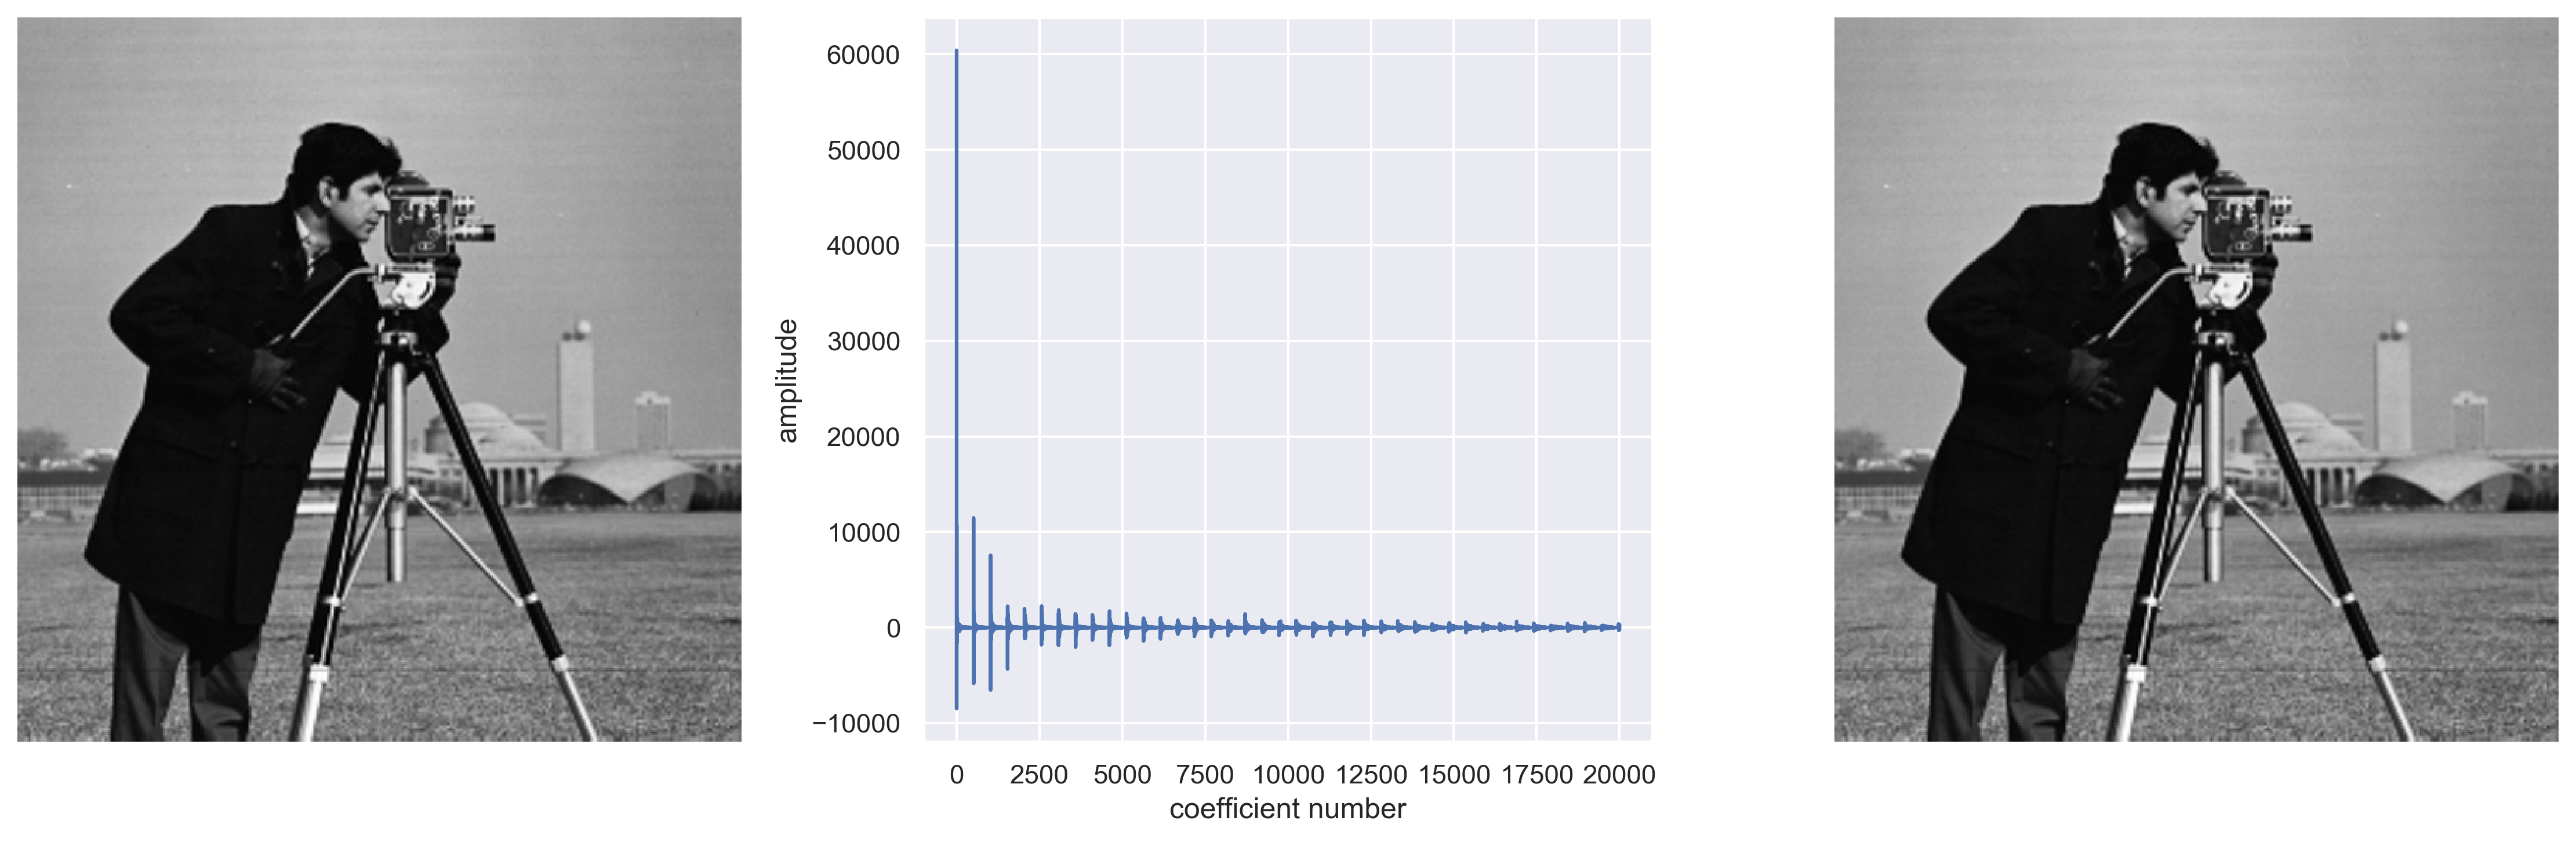
\includegraphics[width=\textwidth]{C2-sparsity.png}
	\caption{Original $512 \times 512$, 8-bit image (left), and a random subset (for better visibility) of its D8 DWT coefficients (middle). Most of the signal energy is concentrated in just a few terms. By discarding all but the 25,000 highest coefficients and performing the inverse transform, the resulting image (right) is perceptually no different from the original.}
	\label{fig:sparsity}
\end{figure}


\section{Incoherence}
\label{sec:incoherence}

Suppose we have two matrices $\bm\Phi$ and $\bm\Psi$ which are involved in the sensing of a signal. As before, $\bm\Psi$ is the sparsifying matrix which converts the signal into a sparse representation, and $\bm\Phi$ is the actual sensing matrix. The coherence $\mu$ between these two bases is expressed as

\begin{equation}\label{eq:coherence}
\mu\qty(\bm\Phi, \bm\Psi) = \sqrt{n} \max_{0 \leq i,j < n} \abs{\innerproduct{\bm\varphi_i}{\bm\psi_j}}.
\end{equation}

In other words, the coherence is the measure of the largest correlation between the column vectors of $\bm\Phi$ and $\bm\Psi$. In compressive sensing, we are interested in low-coherence basis pairs (i.e., basis pairs for which $\mu \rightarrow 1$). For example, in the classical sampling scheme, $\bm\Phi$ is the Dirac basis $\bm\varphi_k(t) = \delta(t - k)$, and $\bm\Psi$ is the DCT basis \eqref{eq:dct}. This basis pair in particular is also called a time-frequency pair and achieves maximum incoherence ($\mu = 1$) regardless of the number of dimensions \cite{Donoho2001}. Additionally, any orthonormal basis $\bm\Phi$ containing independent identically distributed (i.i.d.) entries are also largely incoherent with a fixed basis $\bm\Psi$ \cite{Candes2008b}. The consequence of this is that CS performs most efficiently when sensing with incoherent and random systems.


\section{Reconstruction strategies}
\label{sec:reconstruct}
Another measure of the sparsity of a signal is its $\ell_0$ norm, denoted $\norm{\vec{x}}_0$, which simply counts the number of non-zero coefficients of $\vec{x}$. As such, the goal of the reconstruction stage in CS is to find the sparsest representation of the vector $\vec{x}$ in terms of the sensing matrix $\bm\Phi$ by solving the combinatorial optimization problem

\begin{equation}\label{eq:min-l0}
\min_\vec{x} \norm{\vec{x}}_0 \quad \textrm{subject to} \quad \vec{y} = \bm\Phi \vec{x}
\end{equation}

\noindent which, as the name implies, requires one to enumerate all possible $k$-element combinations of the columns of $\bm\Phi$, and determining the smallest combination which approximates the signal the closest. However, this process quickly becomes intractable even for a modestly-sized signal. This requirement is therefore relaxed by instead minimizing the $\ell_1$ norm

\begin{equation}\label{eq:min-l1}
\min_\vec{x} \norm{\vec{x}}_1 \quad \textrm{subject to} \quad \vec{y} = \bm\Phi \vec{x}
\end{equation}

\noindent where the $\ell_1$ norm is defined as

\begin{equation}\label{eq:l1-norm}
\norm{\vec{x}}_1 = \sum_{i=0}^{N-1} \abs{x_i}
\end{equation}

\noindent and is commonly called the taxicab or Manhattan distance. Most signals encountered in practical situations, however, are not sparse but rather, approximately sparse. As mentioned earlier, any signal measurement will inevitably include some form of noise. Though $\ell_1$ minimization can definitely still be used (by casting it as a convex problem, as in the case of \cite{cvxpy,cvxpy_rewriting}), other algorithms opt for an $\ell_1$-regularized least squares approach as in the case of LASSO \cite{scikit-learn}, whose objective is

\begin{equation}\label{eq:lasso}
\min_{\vec{x}} \frac{1}{2m} \norm{\vec{y} - \bm\Phi\vec{x}}_2^2 + \alpha\norm{\vec{x}}_1
\end{equation}

\noindent where $0 \leq \alpha \leq 1$ is the $\ell_1$ regularization parameter. Greedy algorithms are also a popular approach in this problem, the most common being the sparsity-constrained orthogonal matching pursuit (OMP) \cite{Rubinstein2008}, which has the objective

\begin{equation}
\min_{\vec{x}} \norm{\vec{y} - \bm\Phi \vec{x}}_2^2 \quad \textrm{subject to} \quad \norm{\vec{x}}_0 \leq k.
\end{equation}

\noindent This method enforces the constraint that the reconstructed signal should be, at most, $k$-sparse in the selected coding dictionary $\bm\Phi$. There exist a plethora of algorithms dedicated to the decoding phase of CS. The ones mentioned above are primarily used in this study.
% !TEX root =  main.tex
\chapter{Random sampling-based compressive sensing}
\label{chap:random-cs}

In this chapter, I lay out the groundwork for performing basic compressive sensing techniques which will be repeatedly used and built upon in the following chapters. I also investigate various random properties that take place in the construction of sensing matrices and their potential effect on the reconstruction quality. In order to quantify these properties, I focus primarily on one-dimensional sinusoids, better visualized as audio. In particular, these are signals containing a few known frequency components that do not vary appreciably, if at all, through time.

\section{Test case: Sinusoid}
\label{sec:1dsin}
For the signals of interest, I use the Fourier domain as the sparse representation. I synthesized a C$_5$ piano note (523 Hz)---corresponding to a Nyquist rate of 1046 Hz---using Guitar Pro, with the standard sampling rate of 44.1 kHz and a duration of 1~second. Due to the number of samples, I only worked with the first 1/8th second, corresponding to 5512 samples. This will be the original signal; let's call this signal $\vec{x}$. I then compressively sampled this portion by taking 300 uniformly distributed random measurements, equivalent to a 5\% compression ratio; this will be our compressed vector $\vec{y}$. Figure~\ref{fig:random-sampling} visualizes how these measurements are distributed in time.

\begin{figure}[htb]
	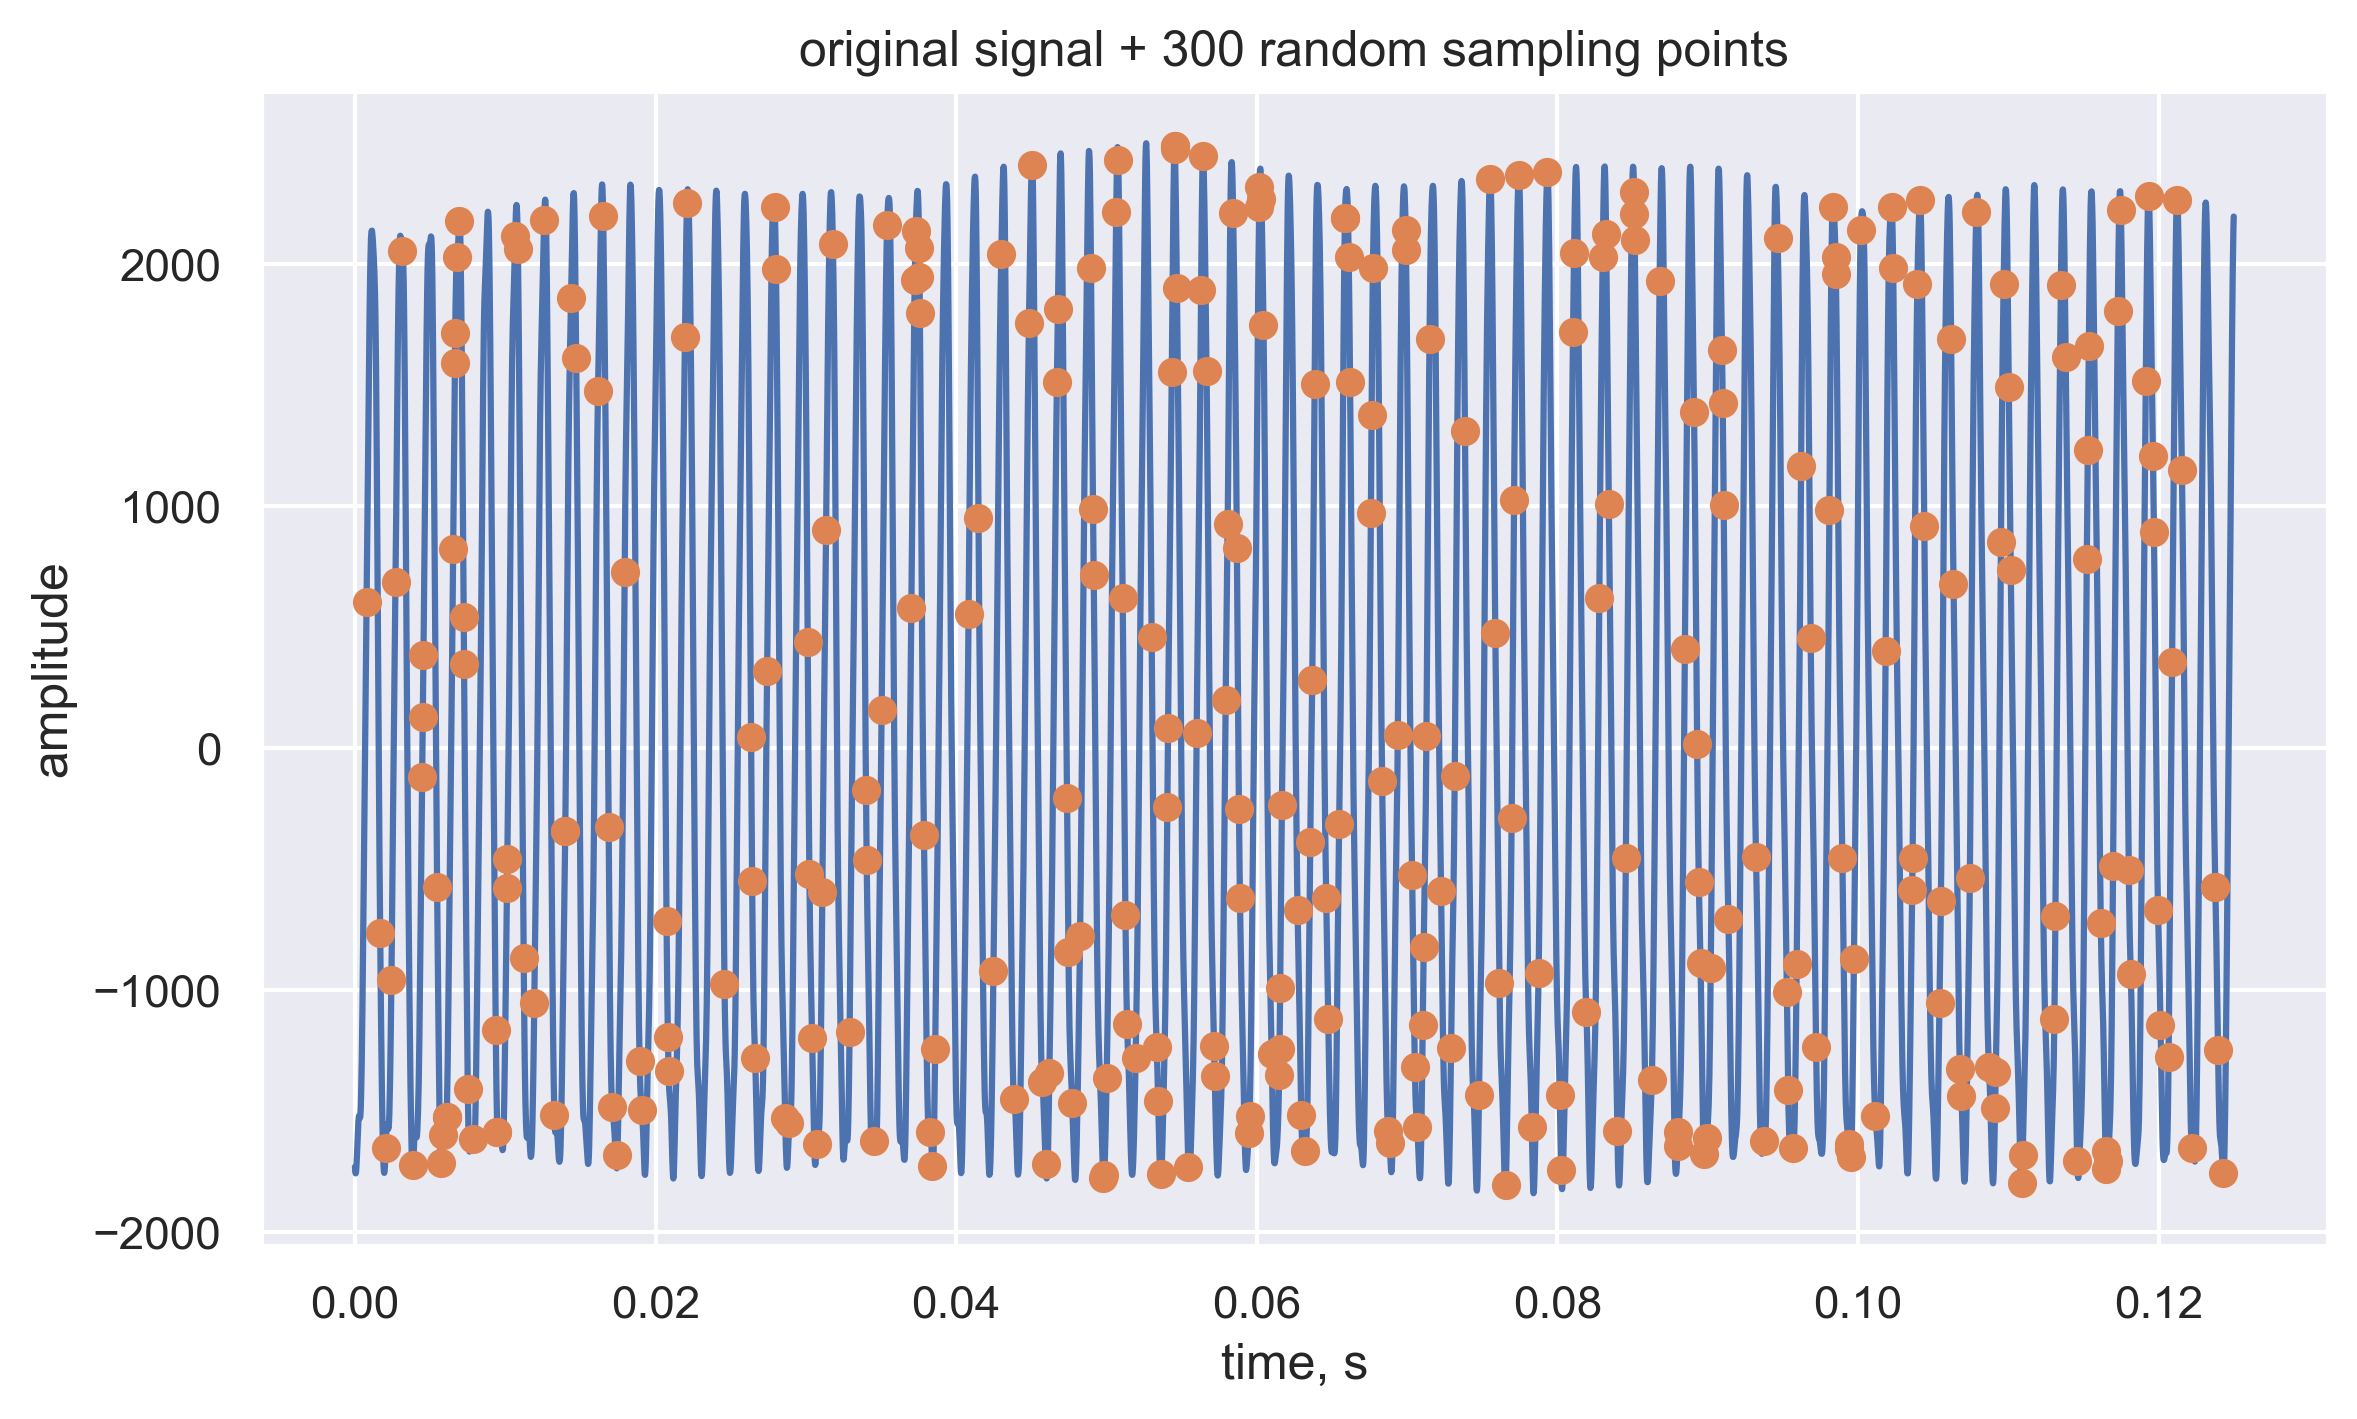
\includegraphics[width=\textwidth]{random_sampling.png}
	\caption{Original synthesized C$_5$ piano note (blue) and random measurements (orange).}
	\label{fig:random-sampling}
\end{figure}

In this model, sampling points consist of a discrete set of indices containing the signal amplitude corresponding to an instantaneous point in time. The random measurements actually point to these indices, which subset the chosen sparsifying basis: in this case, the DCT domain, for simplicity. The same random indices are used to select the rows of the DCT matrix of shape $n \times n$, where $n$ is the signal dimension. I then stack these rows to form the sensing matrix $\vec{A}$; essentially a partial DCT matrix of shape $m \times n$, where $m$ is the number of random measurements. Essentially, I am simulating a sensing device that not only purposely undersamples, but also samples at random, intermittent points in time.

In Chapter \ref{chap:theory}, I discussed an overview of popular algorithms used in CS. For the purposes of comparison in this chapter, I will be focusing on a gradient-based method (LASSO), and a convex optimization-based method (CVXPY). The optimization objectives for these two become

\begin{align}
\mathrm{LASSO}:& \quad \min_{\bm\hat{\vec{x}}} \frac{1}{2m} \norm{\vec{y} - \vec{A}\bm\hat{\vec{x}}}_2^2 + \alpha \norm{\bm\hat{\vec{x}}}_1 \label{eq:random-lasso-objective} \\
\mathrm{CVXPY}:& \quad \min_{\bm\hat{\vec{x}}} \norm{\bm\hat{\vec{x}}}_1 \quad \textrm{subject to} \quad \vec{A}\bm\hat{\vec{x}} = \vec{y} \label{eq:random-cvxpy-objective}
\end{align}

\noindent where $\bm\hat{\vec{x}}$ is the candidate solution, and the optimum value of $\alpha$ is automatically determined via 10-fold cross validation. A detailed implementation is shown in Appendix \ref{appendix:codes}. Figure~\ref{fig:random-compare-algorithms} shows a comparison of the original signal with the reconstructions from the two algorithms in the time and frequency domains. In the time domain, both algorithms appear to have been able to successfully reconstruct the signal, though the CVXPY recovery shows many artifacts. The LASSO algorithm yields a mean-squared error (MSE) of 0.002, while CVXPY yields an MSE of 0.074. In the frequency domain, however, many frequencies are erroneously being recovered by the LASSO method, and more so with the CVXPY method. Because LASSO's $\alpha$ is a hyperparameter, it will need additional tuning to yield a more optimal value.

\begin{figure}[htb]
	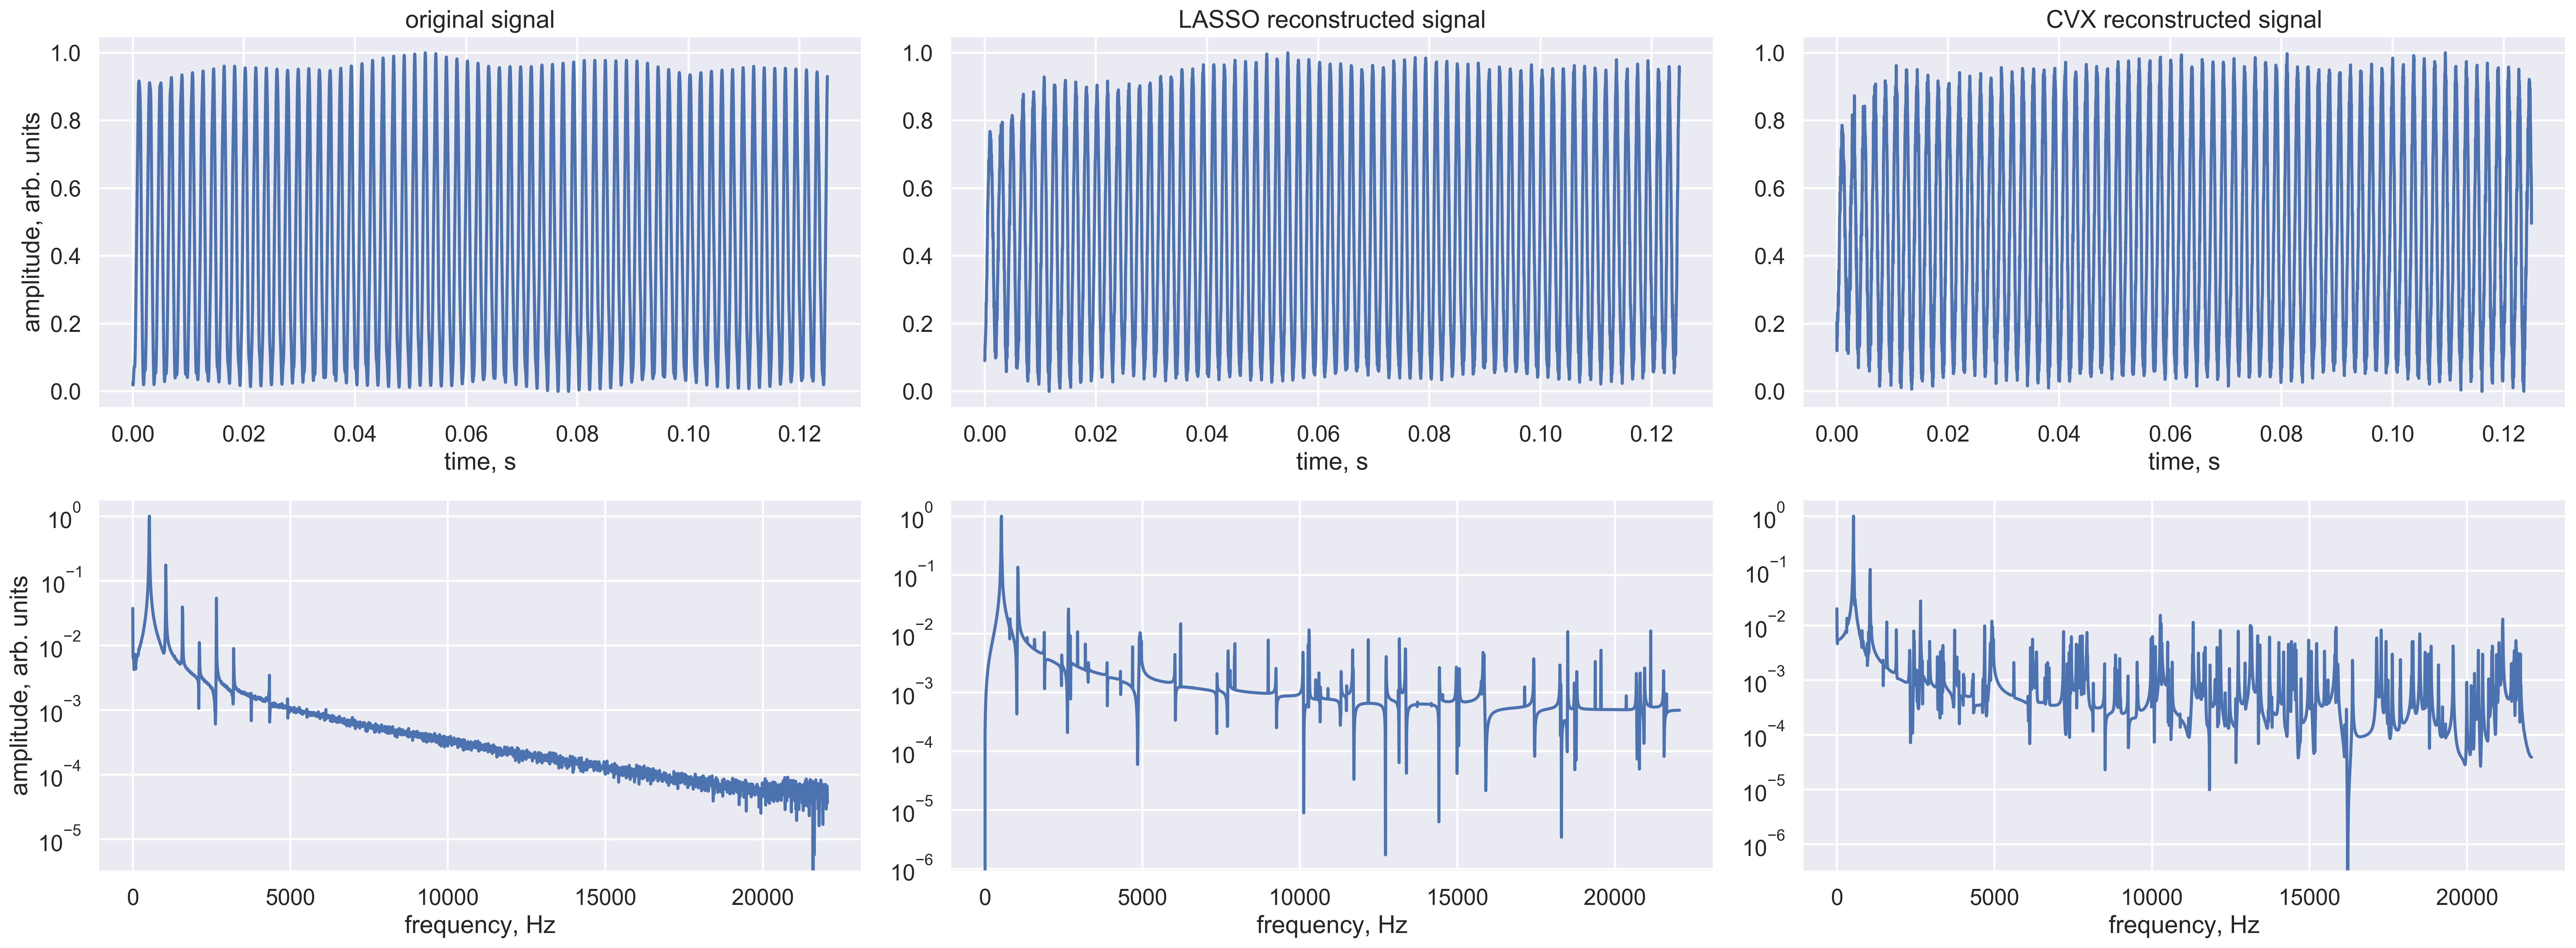
\includegraphics[width=\textwidth]{reconstruction_methods.png}
	\caption{Original signal (left column), LASSO reconstruction (middle column), and CVXPY reconstruction (right column). The top row shows the time domain representation, while the bottom row shows the frequency domain representation.}
	\label{fig:random-compare-algorithms}
\end{figure}


\section{Effect of random distribution on reconstruction error}
\label{sec:random-distro}
So far, I have worked solely with uniformly-distributed random sampling. Here, I investigate and compare the quality of reconstruction (in MSE) in terms of the random distribution. I will be working with two common distributions: the Gaussian and Poisson distributions, as well as the triangular distribution, which is commonly used in audio and image dithering. For each distribution, I generate i.i.d.~random variables and use these to compressively sample the signal. I then evaluate the reconstruction MSE and take the average over 10 iterations to obtain error bars.

\subsection{Uniform}
\label{ssec:random-distro-uniform}
The uniform distribution is given by

\begin{equation}
\label{eq:random-uniform}
U(x) = \begin{cases}
\frac{1}{b - a} & a \leq x \leq b, \\
0 & \mathrm{otherwise}
\end{cases}
\end{equation}

\noindent where $a$ and $b$ are the lower and upper bounds, respectively.

\subsection{Gaussian}
\label{ssec:random-distro-gaussian}
The Gaussian/normal distribution can be generated by

\begin{equation}
\label{eq:random-gaussian}
G(x) = \frac{1}{\sqrt{2\pi\sigma^2}} \exp[-\frac{(x - \mu)^2}{2\sigma^2}]
\end{equation}

\noindent where the parameters $\mu: \mu \in \mathbb{R}$ \& $\sigma^2: \sigma > 0$ are the distribution's mean and variance, respectively.

\subsection{Poisson}
\label{ssec:random-distro-poisson}
The Poisson distribution can be generated by

\begin{equation}
\label{eq:random-poisson}
P(x) = \frac{\lambda^x e^{-\lambda}}{x!}
\end{equation}

\noindent where the parameter $\lambda: \lambda > 0$ is the distribution's mean and variance.

\subsection{Triangular}
\label{ssec:random-distro-triangular}
The triangular distribution is generated by

\begin{equation}
\label{eq:random-triangular}
T(x) = \begin{cases}
0 & x < a, \\
\frac{2(x-a)}{(b - a)(c - a)} & a \leq x < c, \\
\frac{2}{b - a} & x = c, \\
\frac{2(b - x)}{(b - a)(b - c)} & c < x \leq b, \\
0 & x > b
\end{cases}
\end{equation}

\noindent where $a: a \in (-\infty, +\infty)$ is the lower bound, $b: b > a$ is the upper bound, and $c: a \leq c \leq b$ is the mode.

\subsection{Results \& discussion}
\label{ssec:random-distro-rnd}
Due to the computational requirements, I will only work with the first 1/32 seconds of the signal, corresponding to 1378 samples. Figure~\ref{fig:random-pdf} shows the probability density for each distribution.

\begin{figure}[htb]
	\centering
	\begin{subfigure}[h!]{0.49\textwidth}
		\centering
		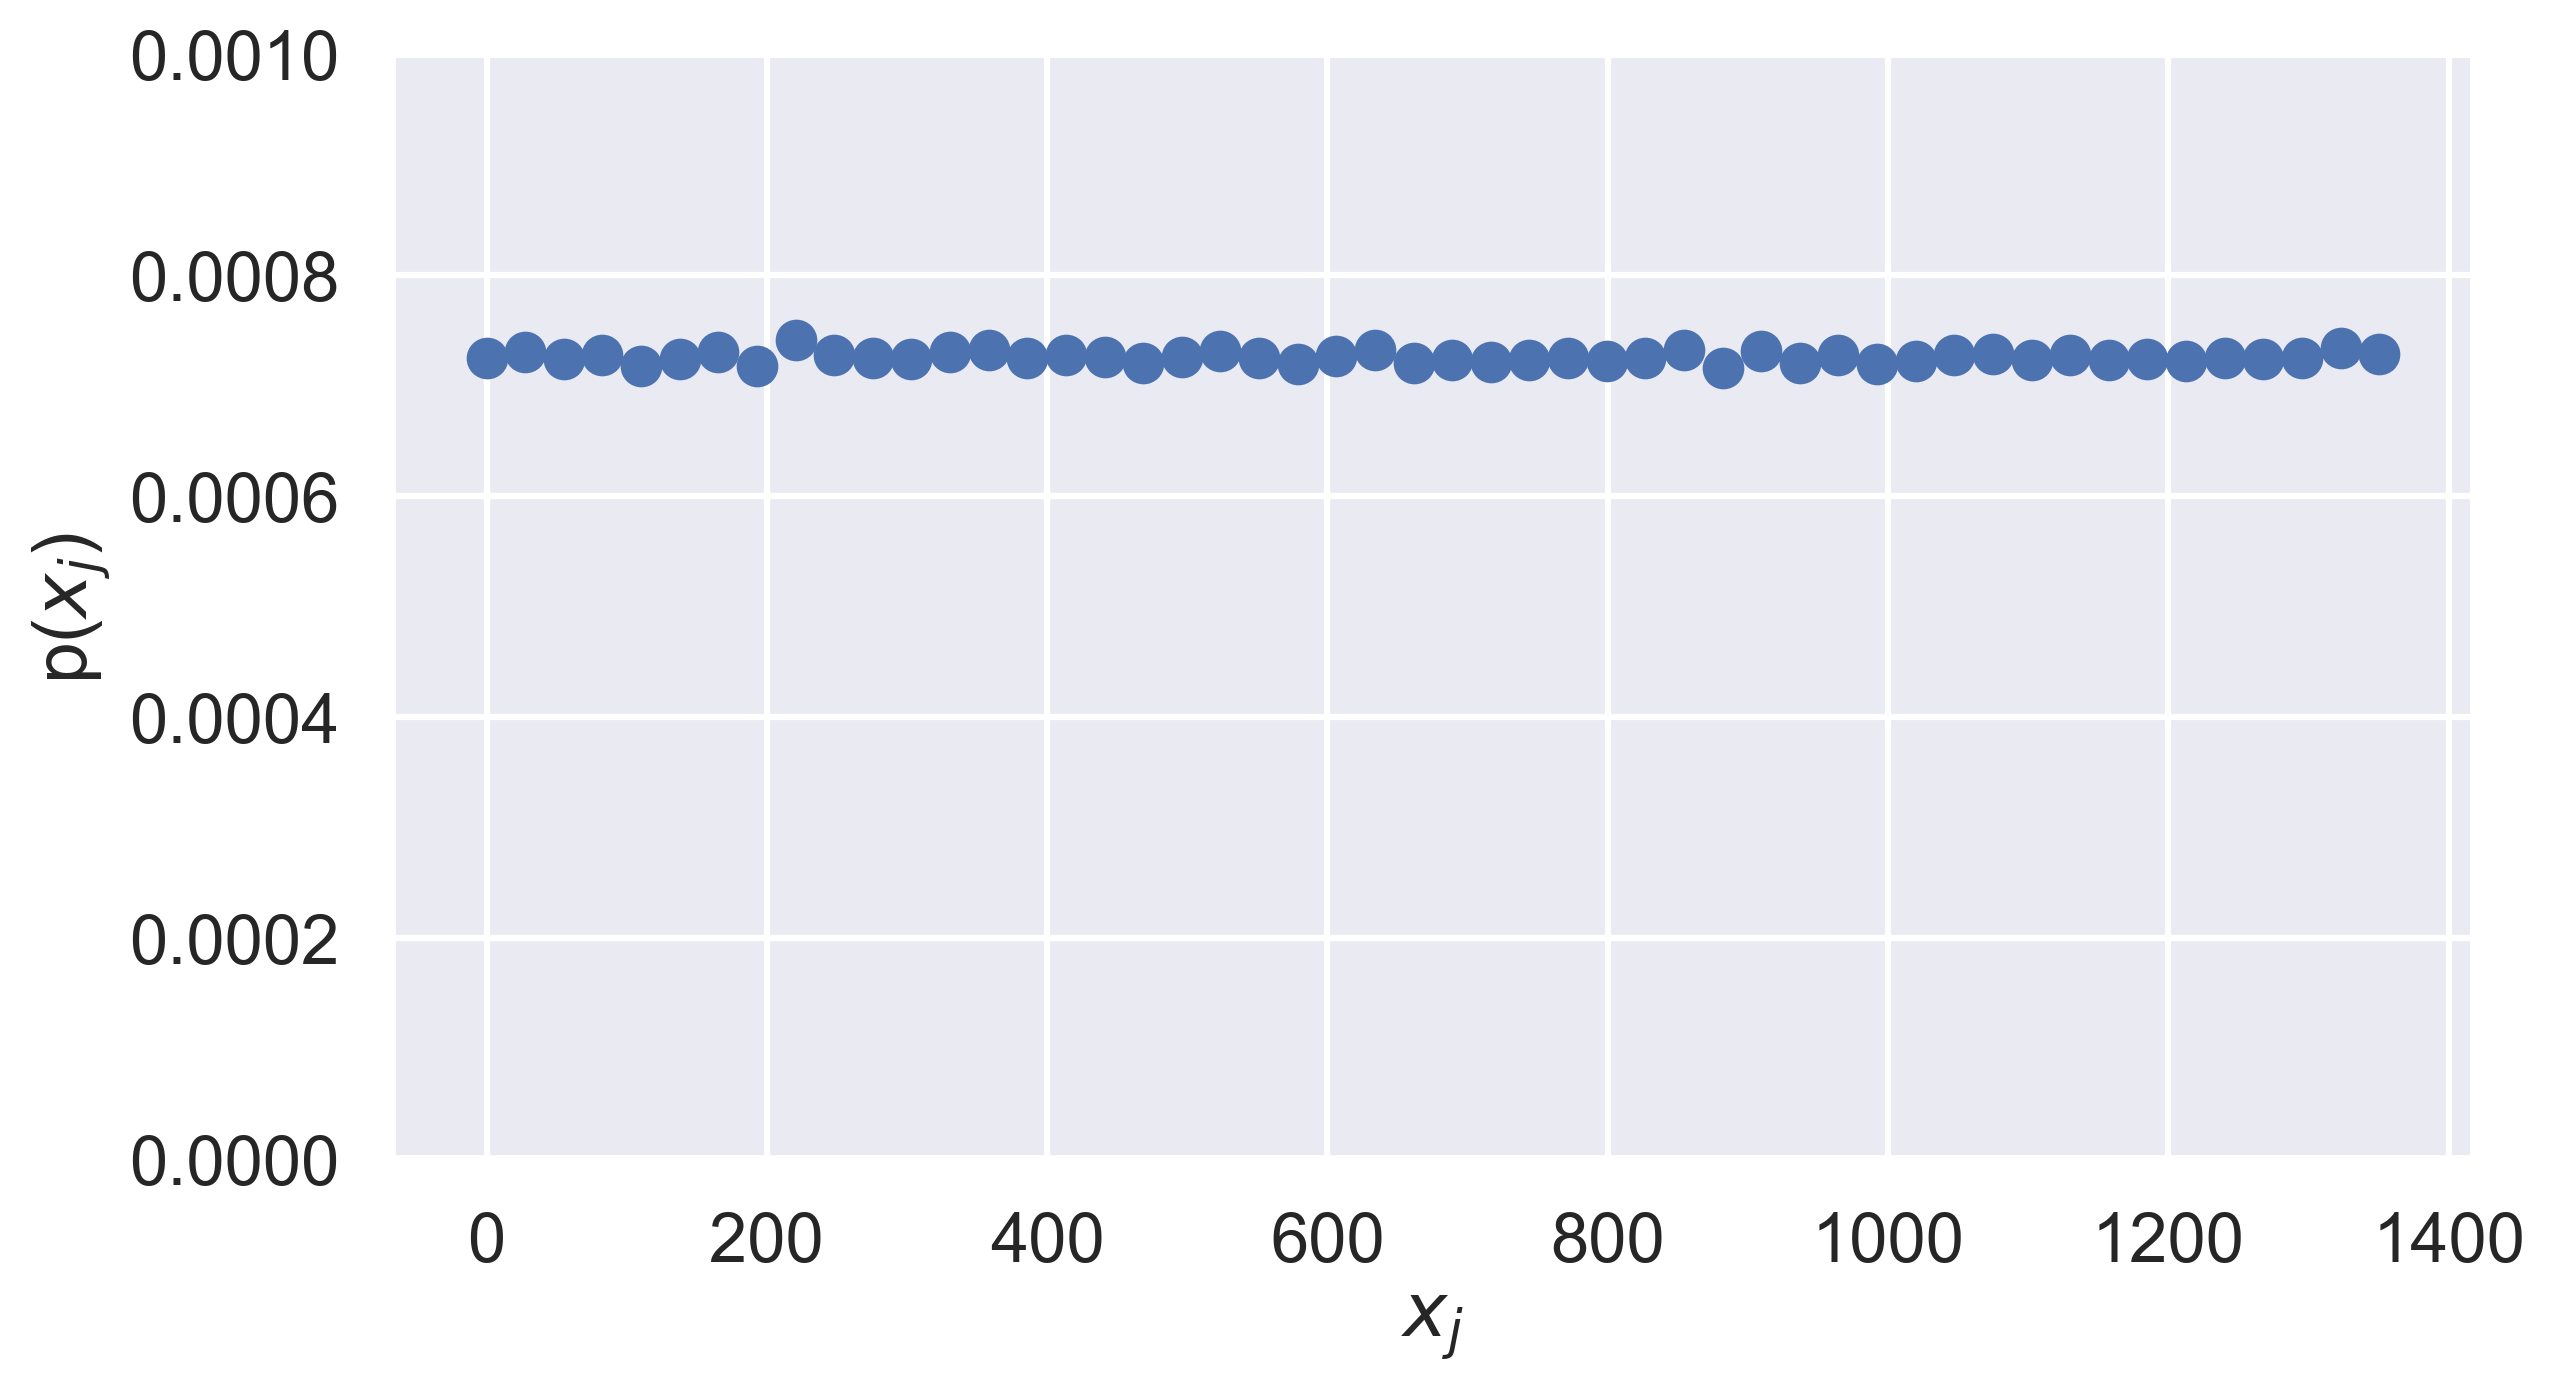
\includegraphics[width=\textwidth]{uniform_random.png}
		\caption{Uniform}
		\label{fig:random-pdf-uniform}
	\end{subfigure}
	\begin{subfigure}[h!]{0.49\textwidth}
		\centering
		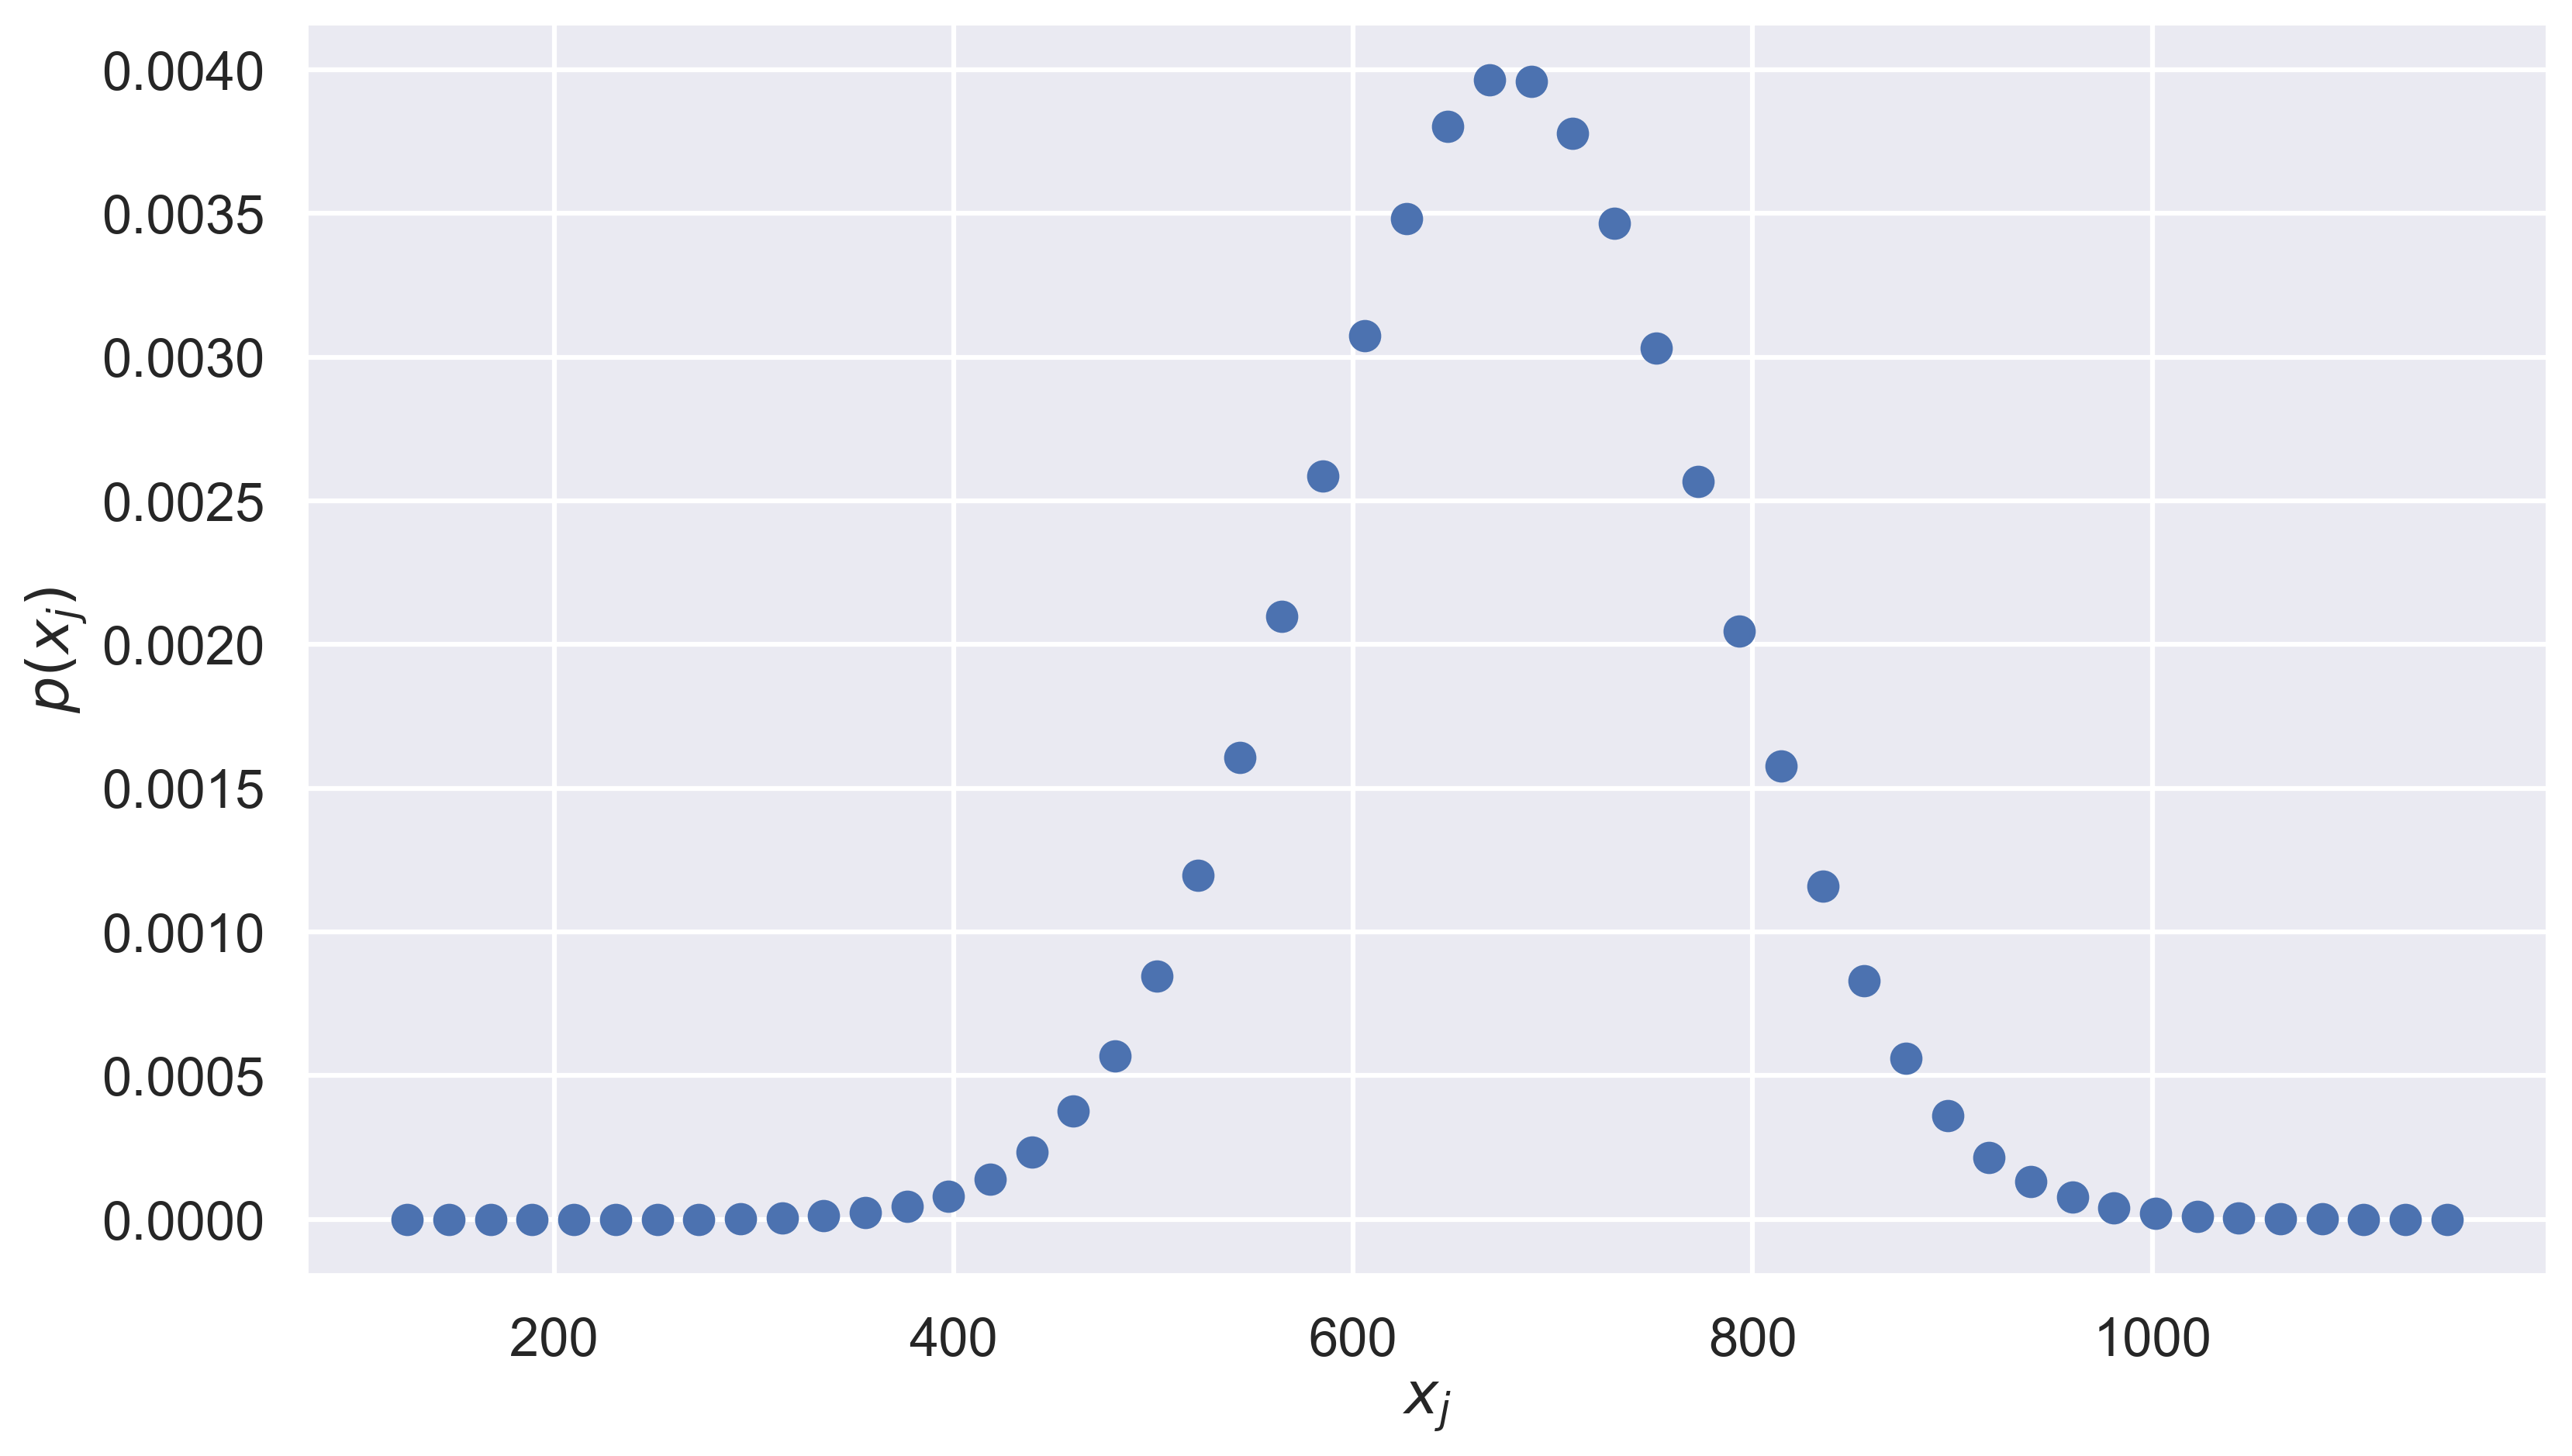
\includegraphics[width=\textwidth]{gaussian_random.png}
		\caption{Gaussian ($\mu = n/2$, $\sigma = 100$)}
		\label{fig:random-pdf-gaussian}
	\end{subfigure}
	\begin{subfigure}[h!]{0.49\textwidth}
		\centering
		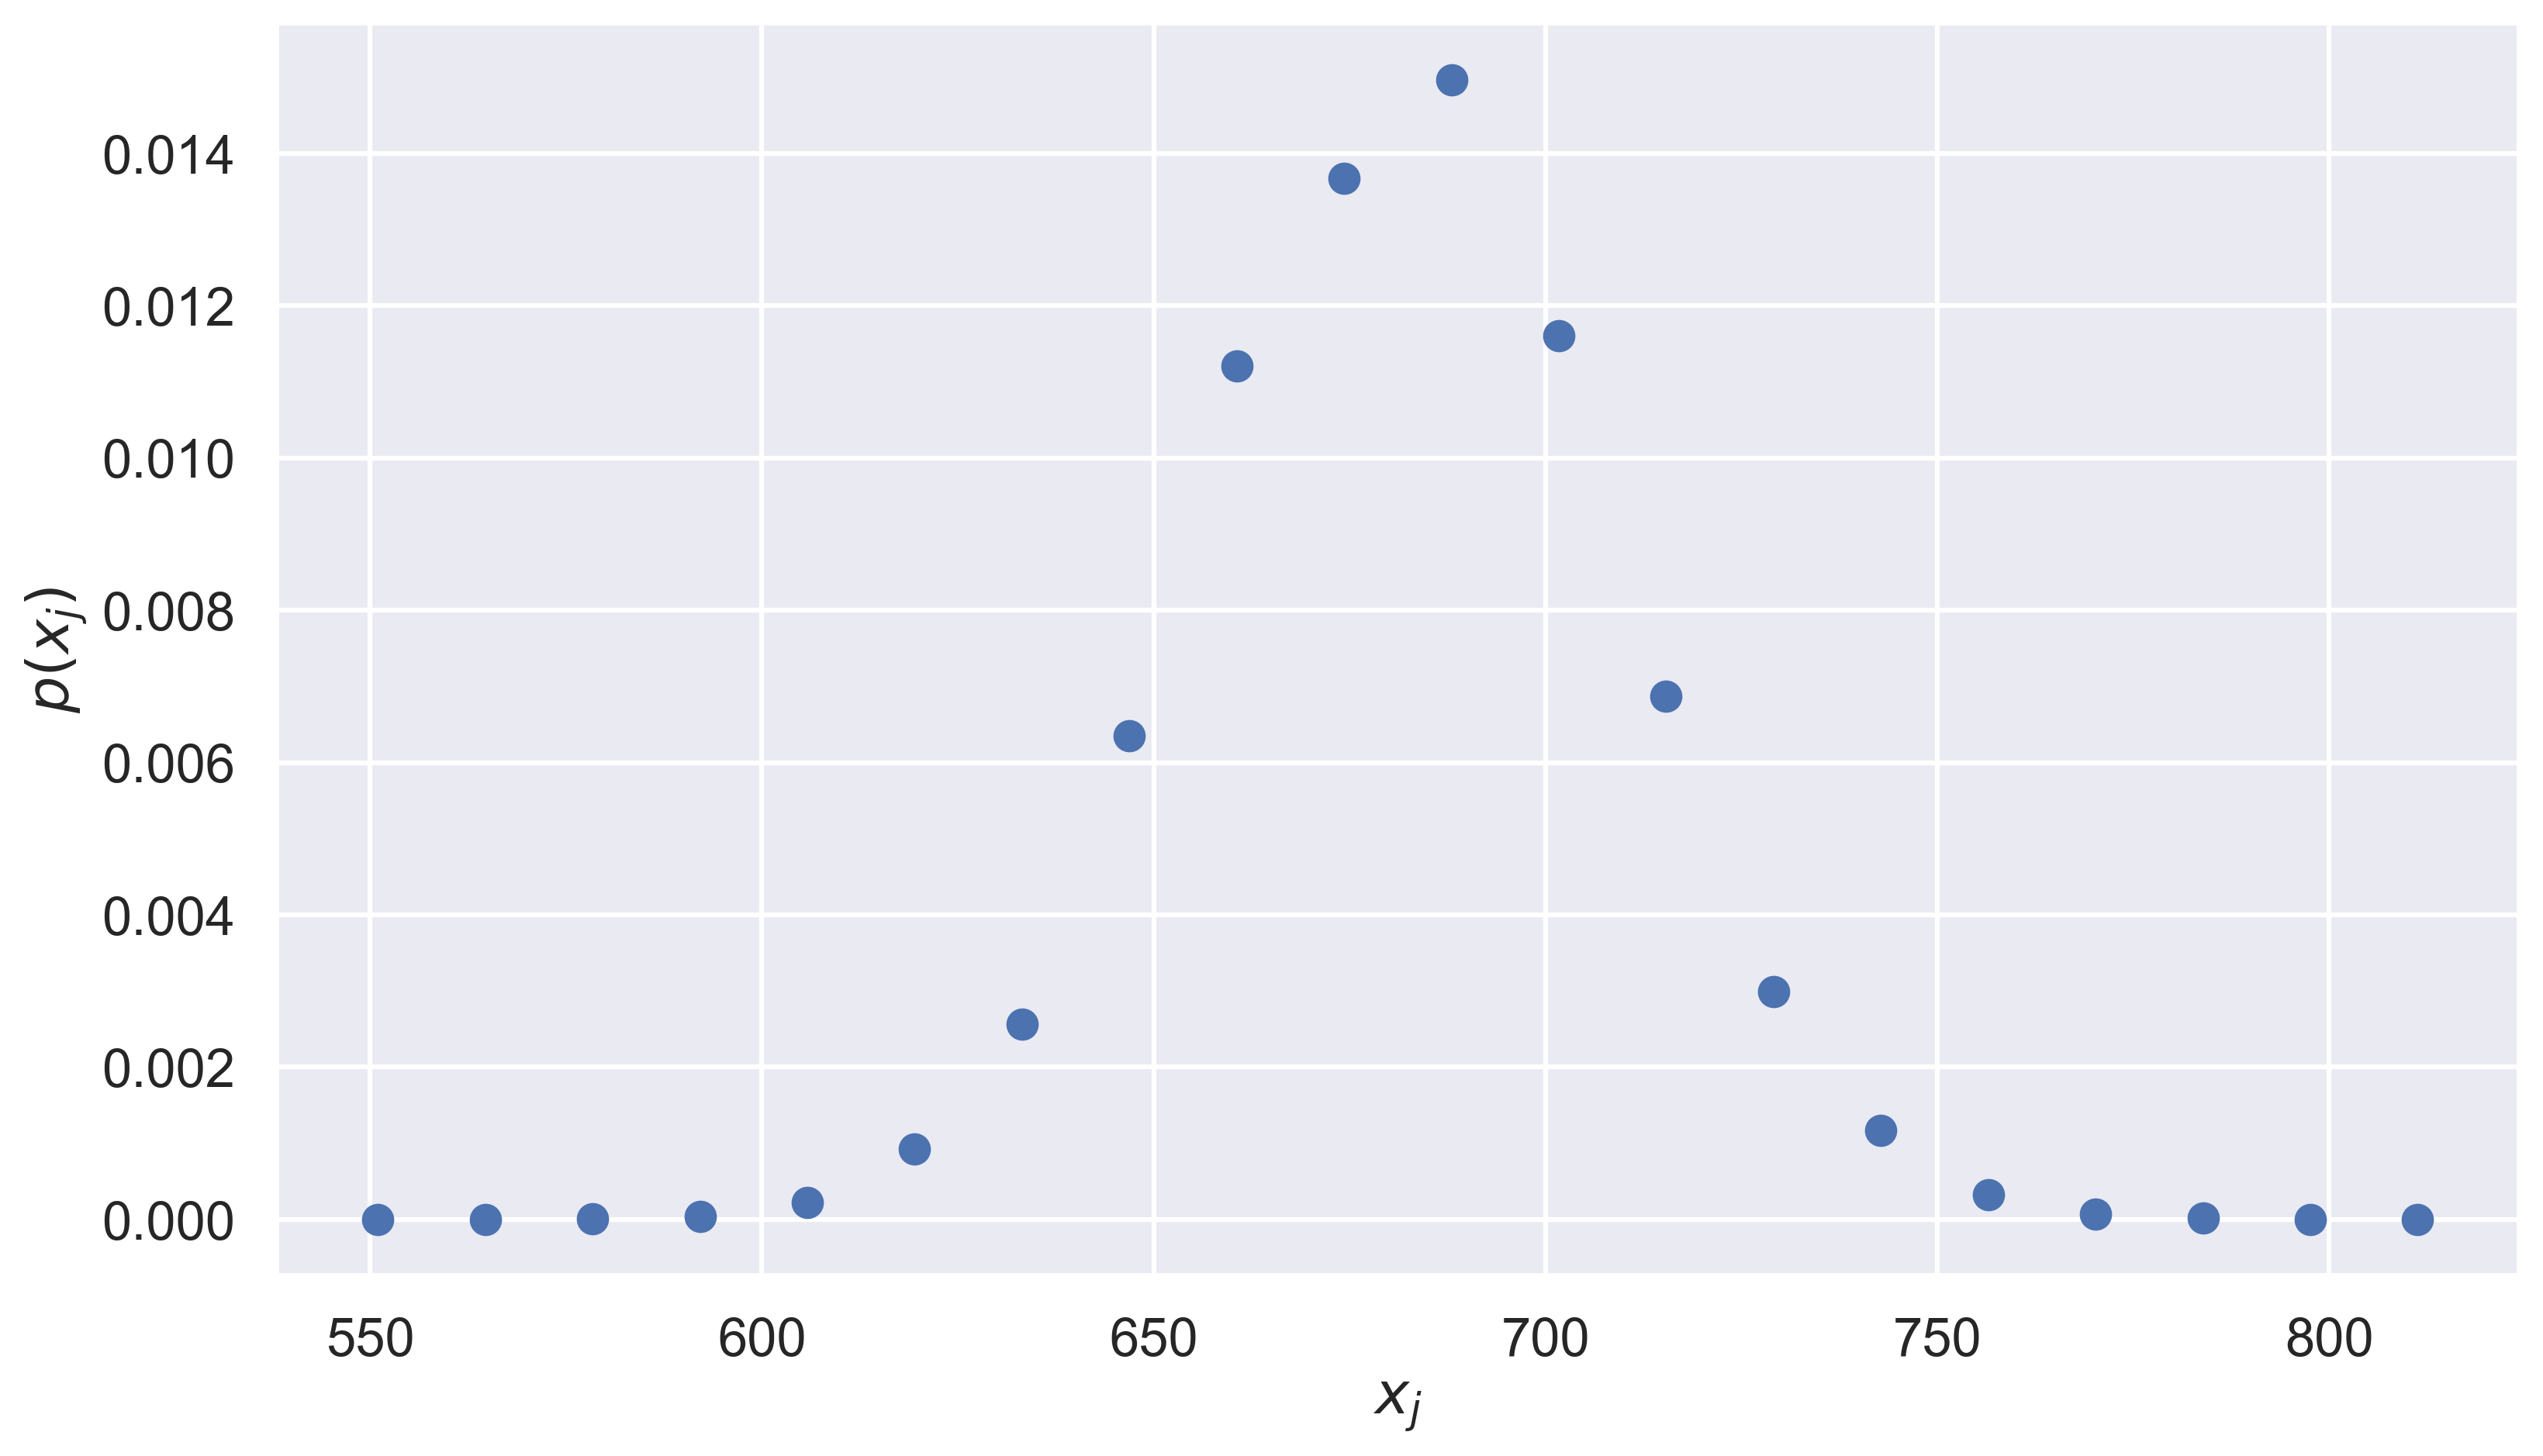
\includegraphics[width=\textwidth]{poisson_random.png}
		\caption{Poisson ($\lambda = n/2$)}
		\label{fig:random-pdf-poisson}
	\end{subfigure}
	\begin{subfigure}[h!]{0.49\textwidth}
		\centering
		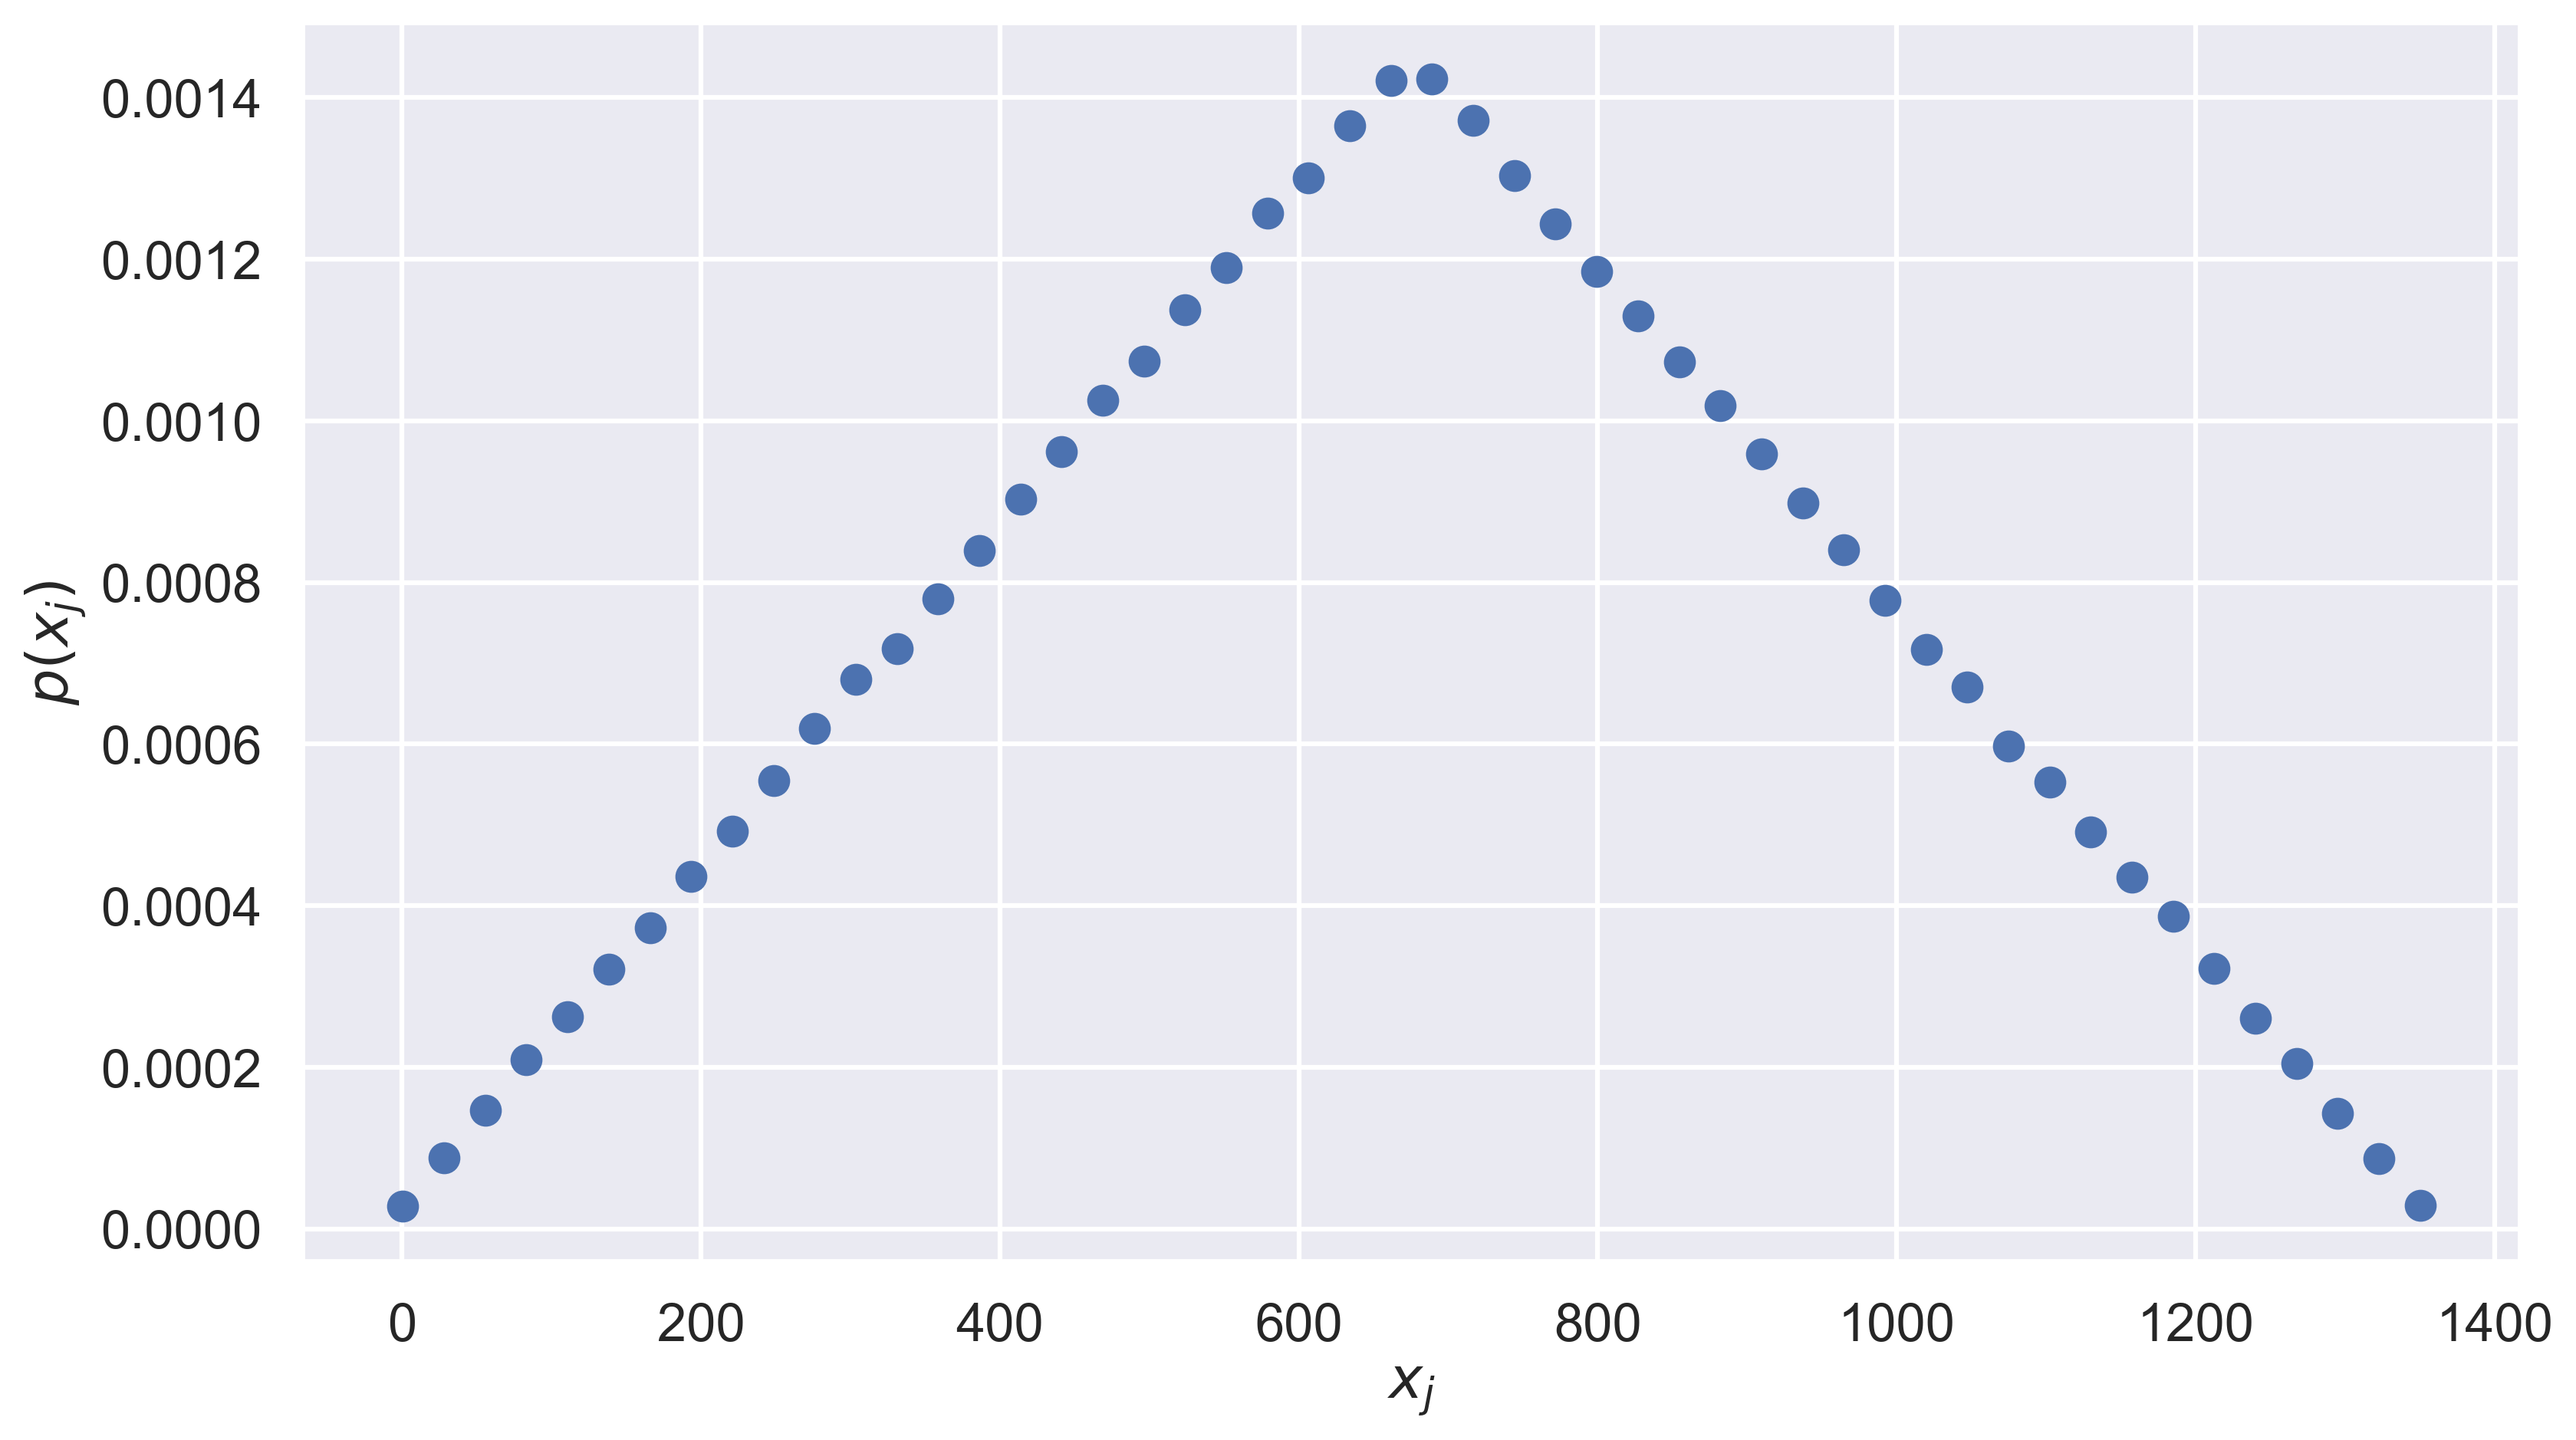
\includegraphics[width=\textwidth]{triangular_random.png}
		\caption{Triangular ($a = 0$, $b = n/2$, $c = n$)}
		\label{fig:random-pdf-triangular}
	\end{subfigure}
	\caption{Probability densities of the different random distributions used in this section, corresponding to the signal indices.}
	\label{fig:random-pdf}
\end{figure}

Figure~\ref{fig:random-mse} shows the MSE evaluated for each random distribution as a function of the fraction of total samples, more aptly referred to as the compression ratio. From this, we can observe that the uniform and triangular distributions give the lowest reconstruction error, but the latter has a more consistent performance across a wide range of compression ratios. They are followed, in order, by the Poisson and Gaussian distributions. One reason for the former's performance is that they are able to completely span the signal with appreciable probability near the bounds, while the latter's probability near the bounds are quickly approaching zero.

\begin{figure}[htb]
	\centering
	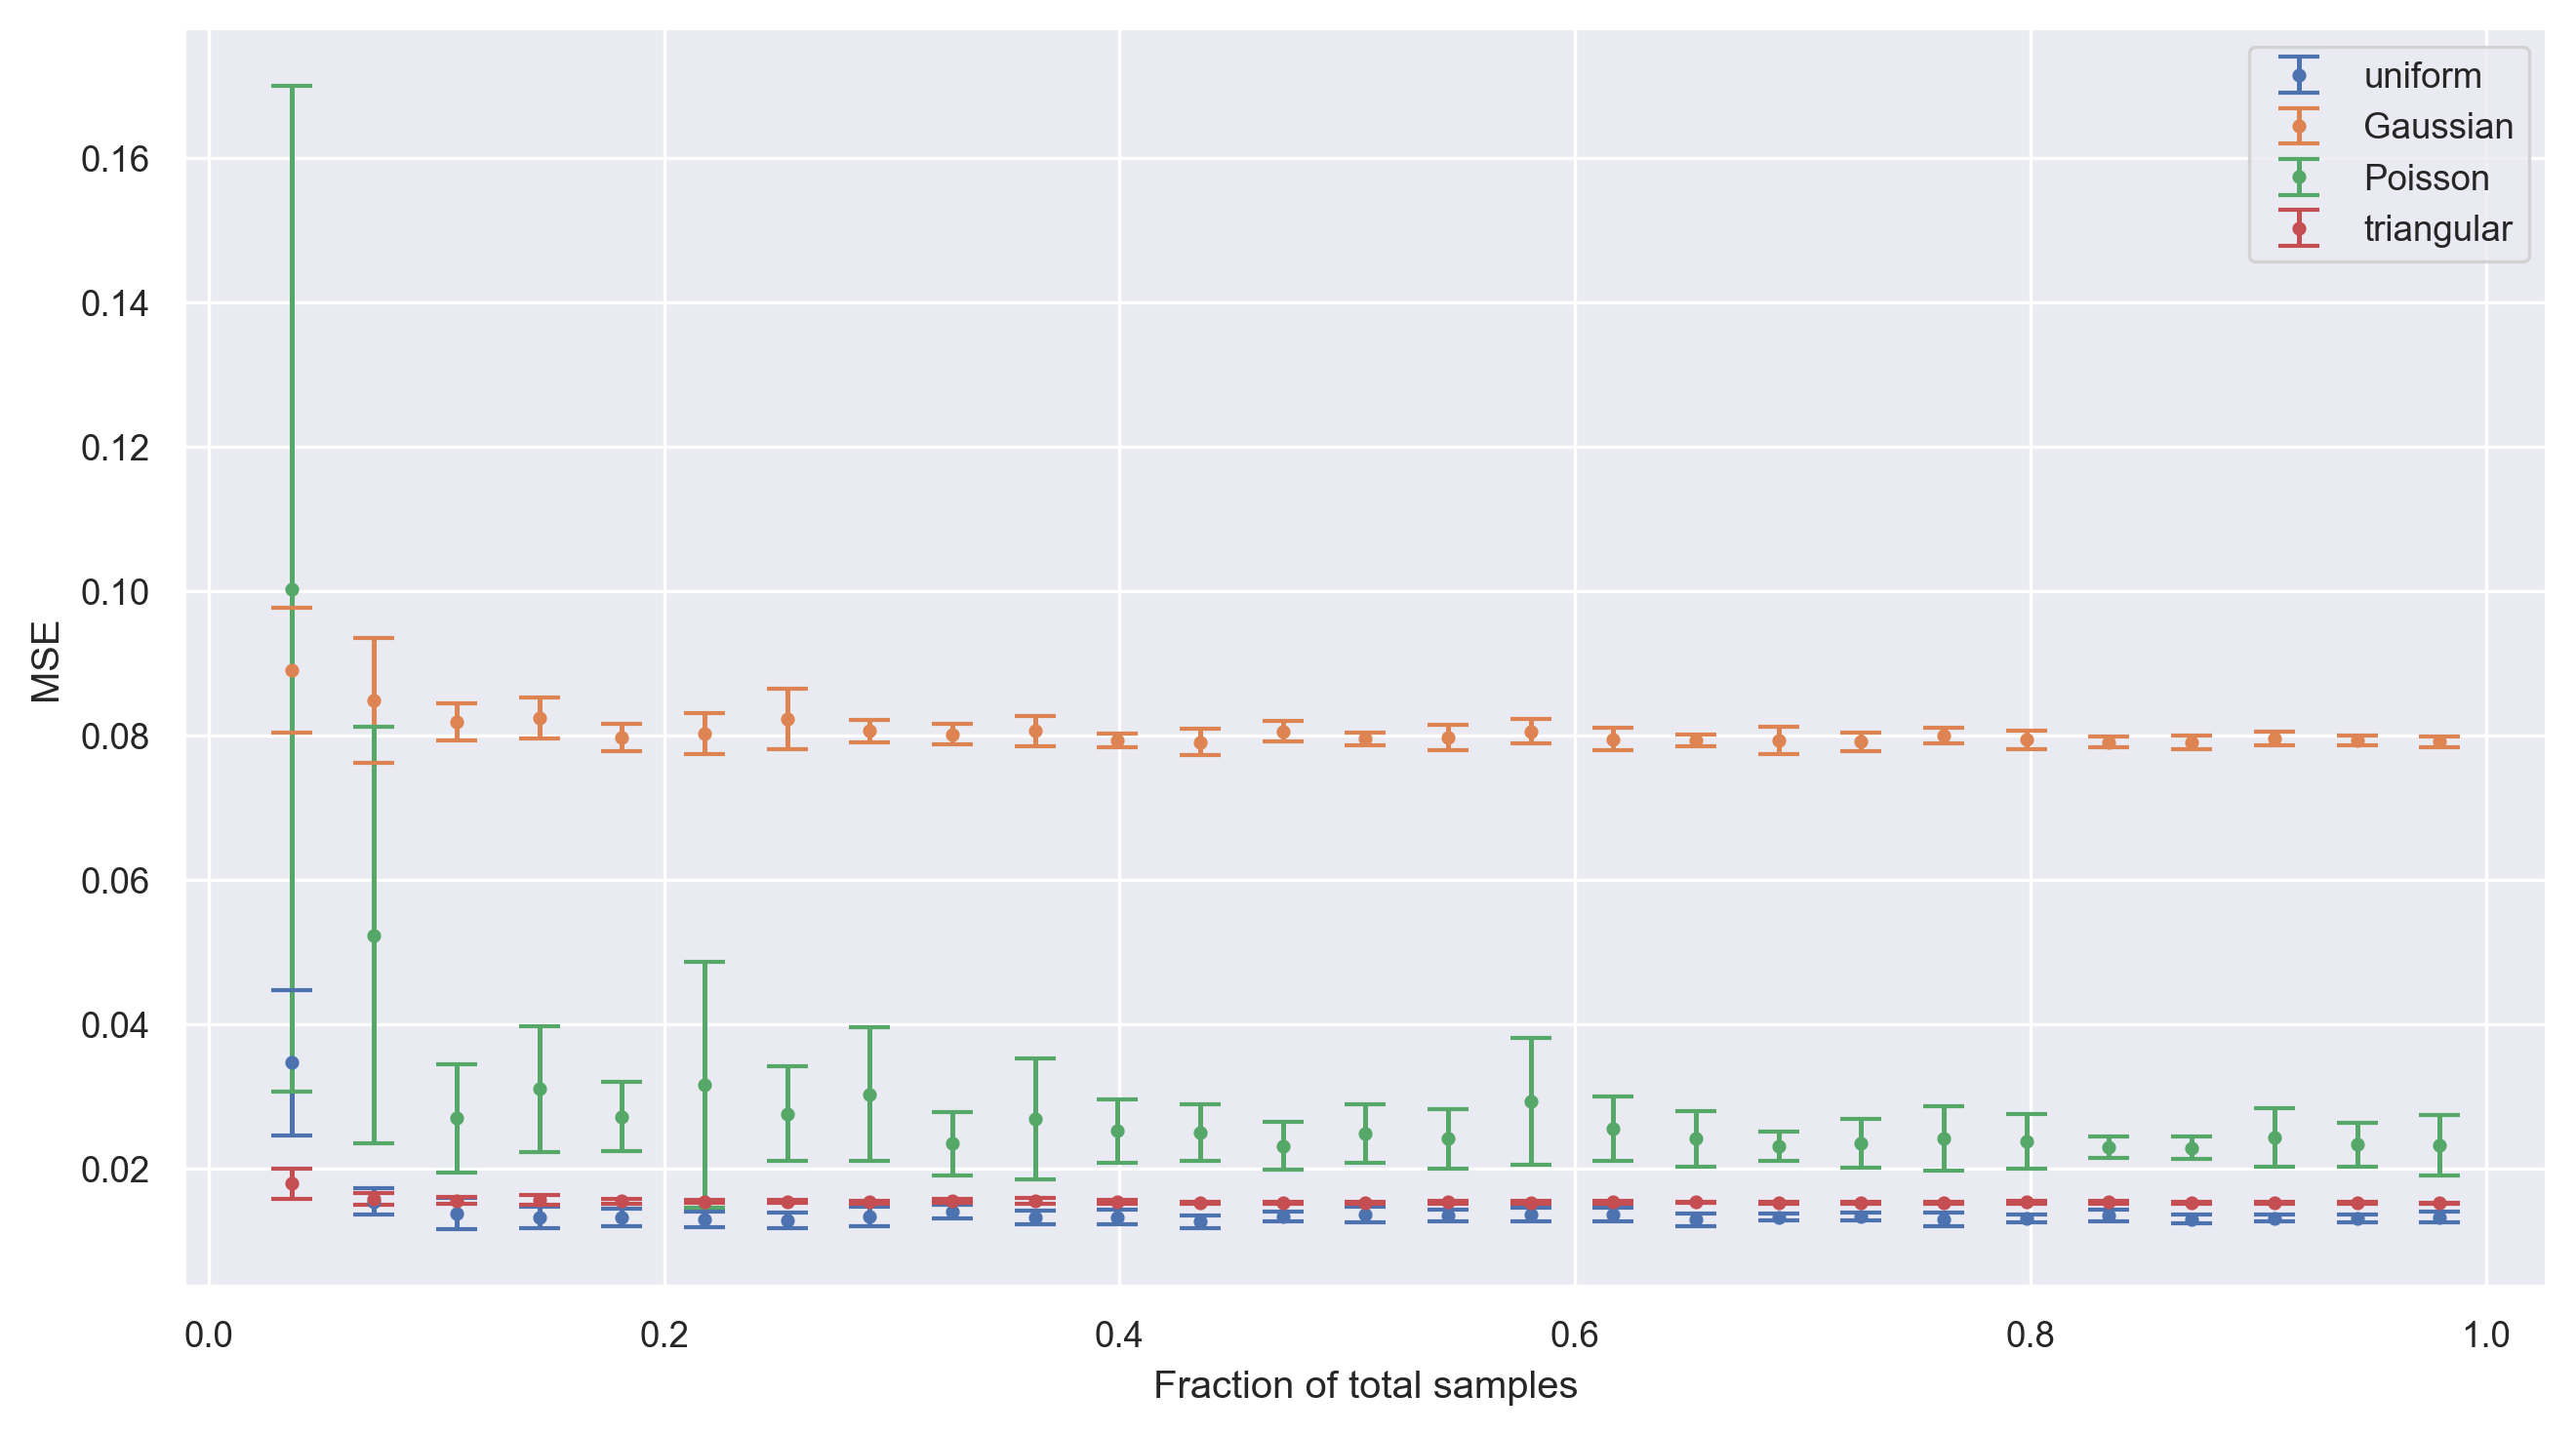
\includegraphics[width=\textwidth]{random_mse.png}
	\caption{Evaluated MSE for each random distribution as a function of compression ratio, average over 10 iterations.}
	\label{fig:random-mse}
\end{figure}

In line with these findings, I will be using uniformly-distributed random variables throughout this study unless otherwise stated. In a later chapters, I will be exploring more on recovering exact frequencies and their harmonics beyond the Nyquist rate in real signals, as well as signals with multiple frequencies. %%could be model or experiment set-up
% !TEX root =  main.tex
\chapter{Image compressive sensing}
\label{chap:image-cs}


One of the more intuitive applications of CS lies in spatial signals as it is easier to visualize. In this scheme, the process can be simplified either by flattening it to one dimension and processing it in its entirety, or maintaining its dimensionality and processing it by patches. The general workflow that arises from image CS is as follows:

\begin{enumerate}
	\item Define the compression ratio $m/n$, where $n$ is the signal size, and $m$ is the desired size of the compressed signal.
	\item Draw $m$ random indices from the signal without replacement and store this as a sample sequence $\bm\xi$.
	\item Extract the row vectors of the desired $n \times n$ sparsifying basis $\bm\Psi$ indexed by $\bm\xi$, and stack these to form the sensing matrix $\bm\Phi$ (i.e., $\bm\Phi = \bm\Psi_{\bm\xi}$)
	\item With the desired reconstruction algorithm, perform the optimization \eqref{eq:min-l1} to obtain the reconstructed signal $\bm\hat{\vec{x}}$.
\end{enumerate}

In the case of high-definition images (whose shortest side is at least 720 pixels), it is usually more practical and yields better results if the image is processed in patches.


\section{Test case: Sinusoidal pattern}
\label{sec:2dsin}
As mentioned in Chapter~\ref{chap:theory}, the most commonly used sparse representation domain for images is the Fourier domain, referred to in some fields as $k$-space. In this space, signals are represented as a linear superposition of a finite number of sinusoidal patterns. In Fig.~\ref{fig:2dsin}, $64 \times 64$ pixel sinusoidal patterns are generated, corresponding to sine waves traveling horizontally, vertically, and diagonally, as well as an egg tray pattern. In each case, all frequency components are 4 Hz. Figure~\ref{fig:2dsin-masked} visualizes the compressed image when a random sample of 5\% is taken from the signal. The actual compressed signal that is seen by the reconstruction algorithm is a one-dimensional sequence containing only the information from the points being sampled. Orthogonal matching pursuit (OMP) was used for reconstruction, which is a greedy algorithm that finds the combination of basis vectors which best represents the signal (similar to matching pursuit), but in addition, the residual at each iteration is recomputed using an orthogonal projection on the set of previously selected basis vectors \cite{Mallat1993}. Its objective function is

\begin{equation}\label{eq:omp}
\arg\min_{\vec{x}} \norm{\vec{y} - \bm\Phi \vec{x}}_2^2 \quad \textrm{subject to} \quad \norm{\vec{x}}_0 \leq \gamma
\end{equation}

\noindent where $\gamma$ is a hyperparameter which controls the maximum allowable number of non-zero coefficients. The \texttt{Scikit-learn} implementation sets this value to 10\% of the number of samples by default \cite{scikit-learn}. Evaluation of the mean-squared error (MSE) for the pure horizontal and pure vertical sine waves, as well as the egg tray pattern yields a value that is practically negligible ($\approx 10^{-31}$); the reconstruction is exact. On the other hand, the reconstructed diagonal sine wave yields an MSE of $10^{-3}$---still quite small, but mild distortion can be observed at the image boundaries. This is due to the fact that the information at hand is finite, and so is the window size which, in this case, is the same size as the signal itself.

\begin{figure}[htb]
	\centering
	\begin{subfigure}{\textwidth}
		\centering
		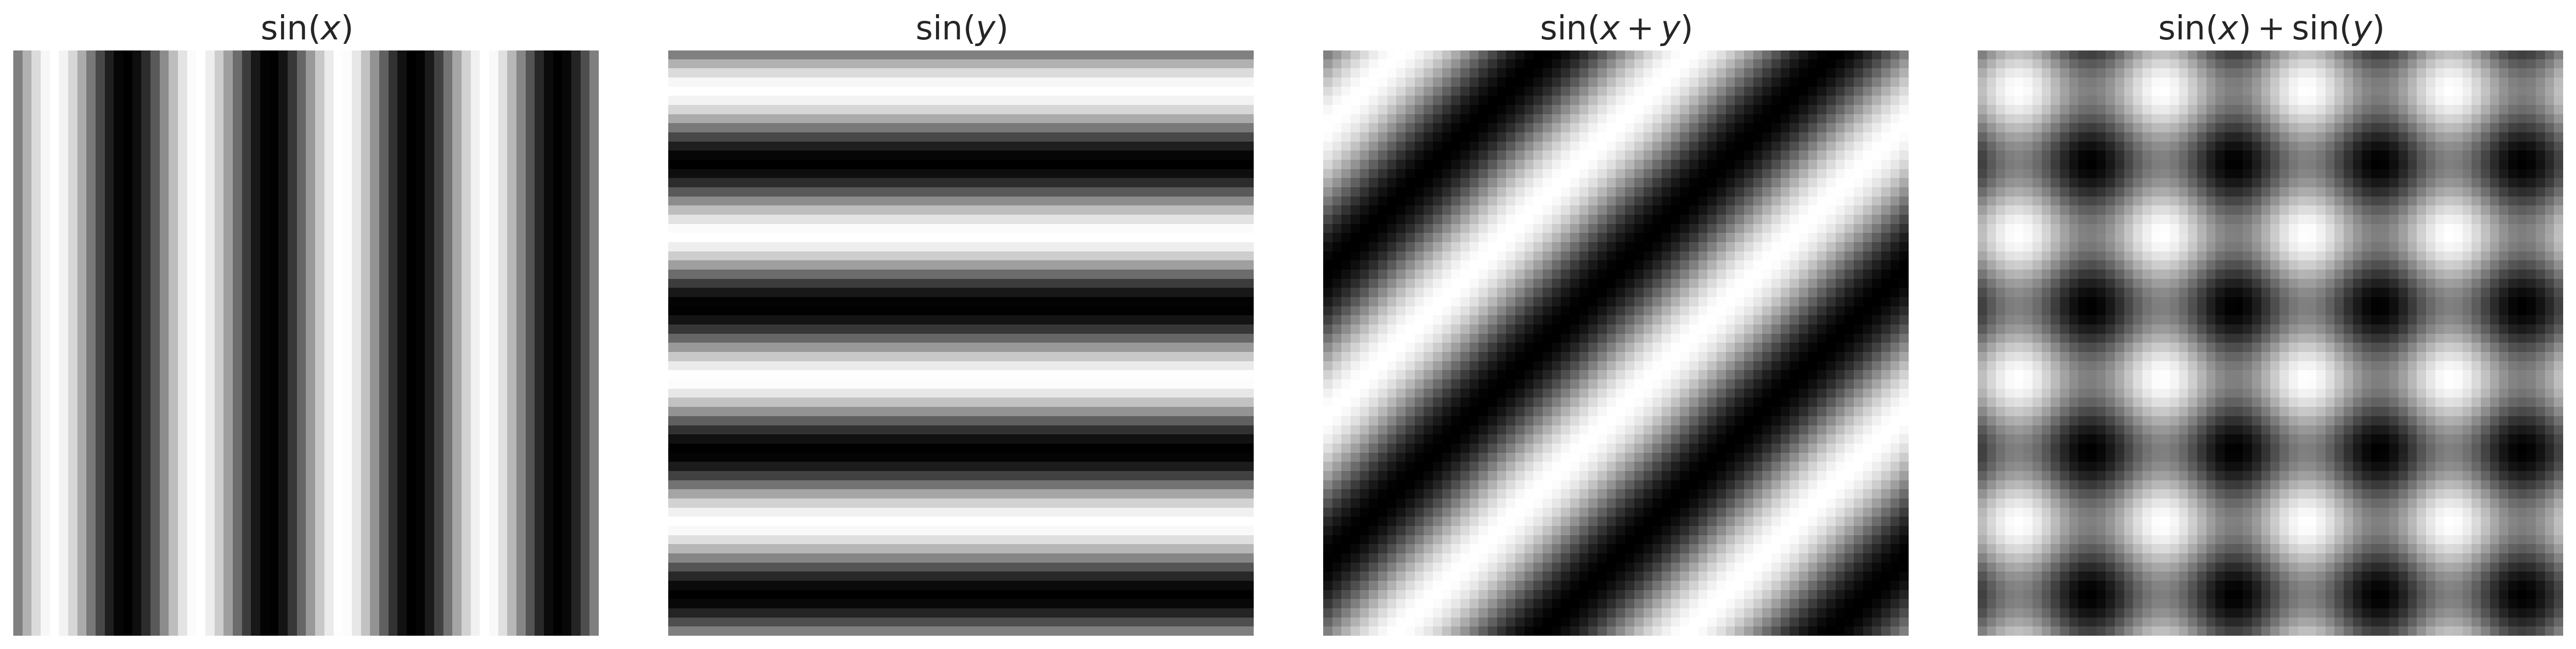
\includegraphics[width=\textwidth]{2dsin.png}
		\caption{Test 2D sinusoid patterns.}
		\label{fig:2dsin}
	\end{subfigure}
	\begin{subfigure}{\textwidth}
		\centering
		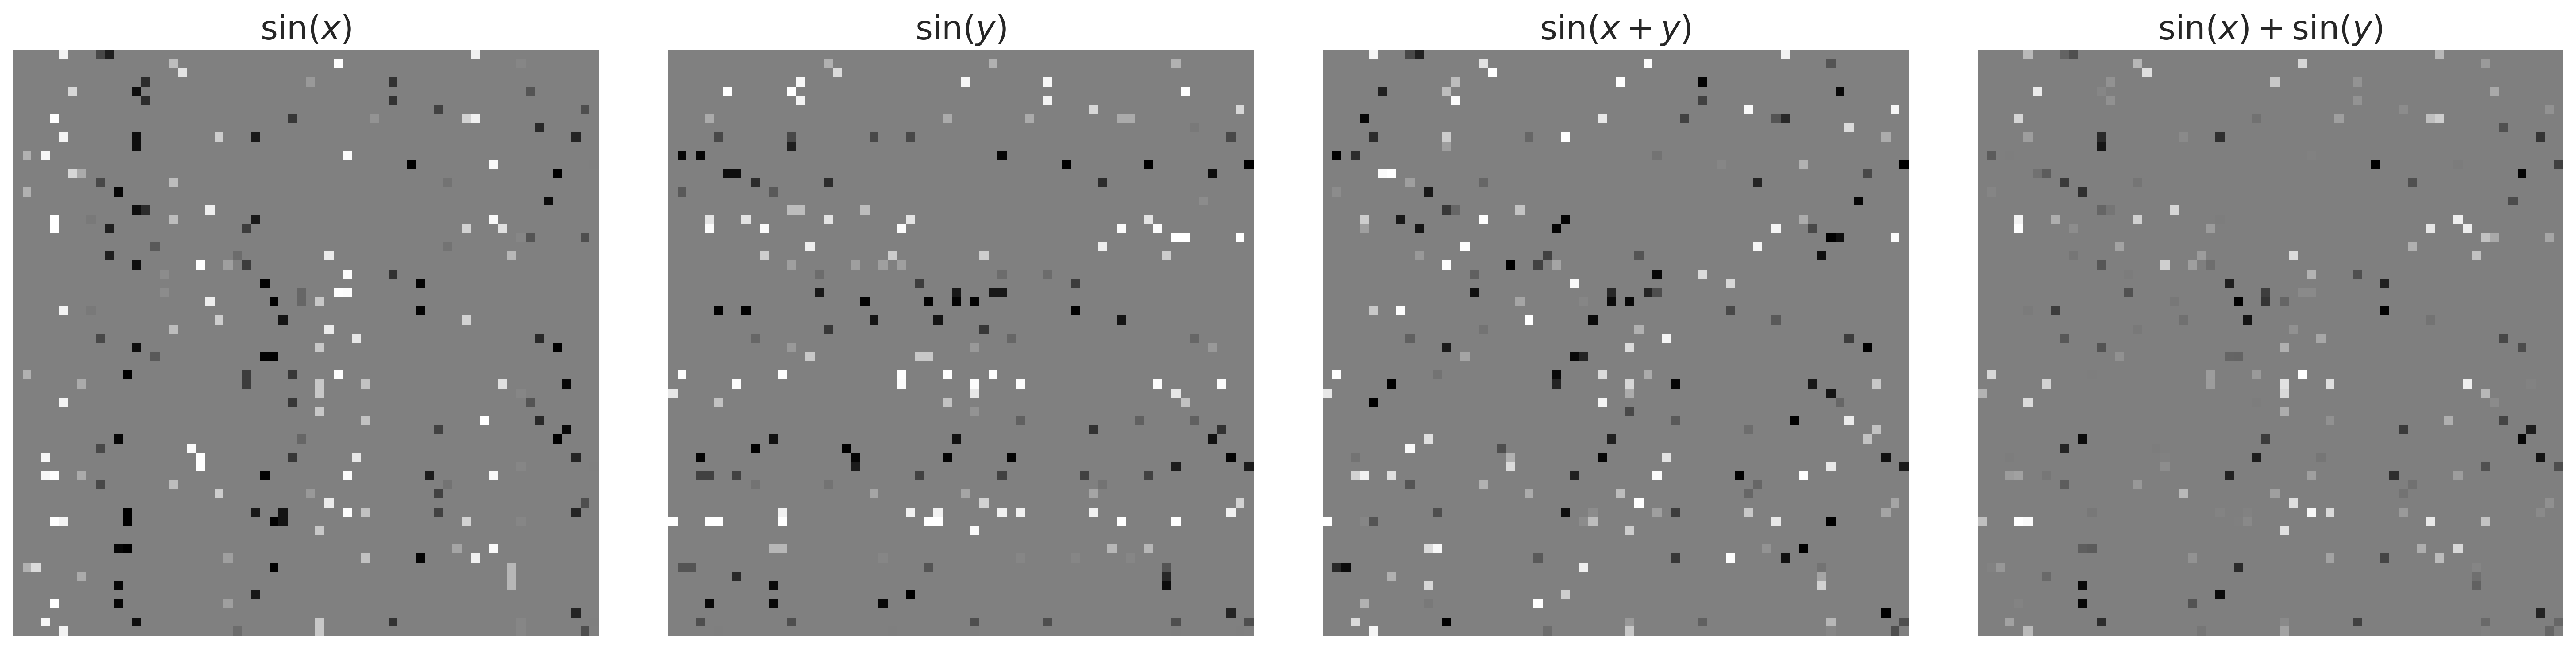
\includegraphics[width=\textwidth]{2dsin-masked.png}
		\caption{Visualization of sinusoid patterns with compression ratio of 5\%.}
		\label{fig:2dsin-masked}
	\end{subfigure}
	\begin{subfigure}{\textwidth}
		\centering
		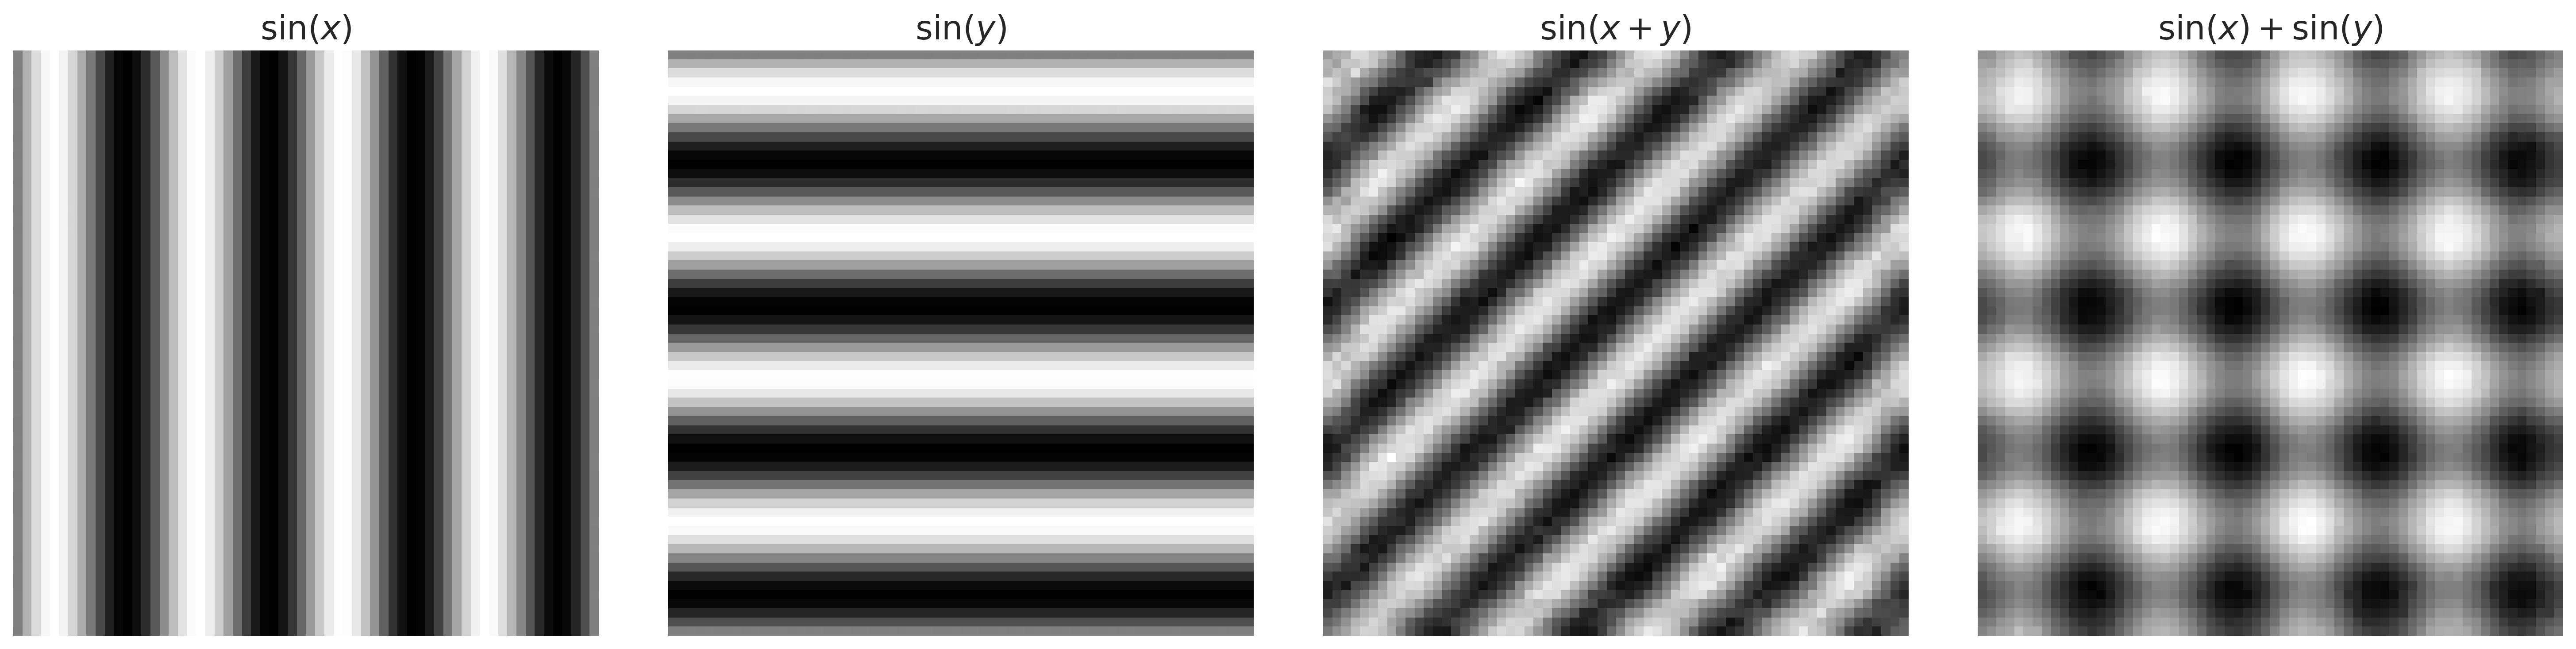
\includegraphics[width=\textwidth]{2dsin-recovered.png}
		\caption{Reconstruction from 5\% of samples.}
		\label{fig:2dsin-recovered}
	\end{subfigure}
	\caption{Test $64 \times 64$ pixel 2D sinusoid patterns corresponding to vertical sinusoids, horizontal sinusoids, diagonal sinusoids, and egg tray pattern. All frequency components are 4 Hz.}
	\label{fig:test-2dsin}
\end{figure}


\section{Image with multiple sinusoids}
\label{sec:2dmultisin}

\subsection{Pre-processing}
\label{ssec:image-multi-preprocess}
For this section, the image used is M.C. Escher's \textit{Relativity}, an example of a more complex image but consisting of dominant sinusoidal patterns that are made apparent when you zoom in. The original image has dimensions of $1600 \times 981$ pixels, for a total of 1,569,600 pixels. Following the procedure with the previous section, this would require the construction of a 1,569,600 $\times$ 1,569,600 sparsifying matrix containing $\approx 2 \times 10^{12}$ entries. Assuming that the matrix would be stored as 32-bit floating point numbers, this process alone would take up $\approx 8$ GB of memory, and it would be highly impractical to process similarly-sized images as a whole. The workaround is to split it into smaller, manageable patches. 

\subsection{Processing}
\label{ssec:image-multi-process}
For this image in particular, it was first resized to $1600 \times 976$ pixels so that it could be equally divided into a grid of $16 \times 16$, each with a dimension of $100 \times 61$ pixels. After compressively sampling each patch at 40\% compression ratio, reconstruction was performed using the Embedded Conic Solver (ECOS) of the Convex Optimization Python library (CVXPY), which recasts \eqref{eq:min-l1} as a convex problem and directly minimizes the $\ell_1$ norm \cite{ecos,cvxpy,cvxpy_rewriting} and thus, is significantly slower compared to OMP.

\subsection{Reconstruction evaluation}
\label{ssec:image-multi-error}
To quantify the reconstruction quality, the Structural Similarity Index (SSIM) \cite{Wang2004} was used. This is a perception-based model that takes into account perceptual factors such as luminance, contrast, and structure. SSIM is calculated on windows in the image, and is defined as

\begin{equation}
\label{eq:ssim}
\mathrm{SSIM}(\vec{x}, \bm\hat{\vec{x}}) = \frac{(2\mu_{\vec{x}}\mu_{\bm\hat{\vec{x}}} + c_1) (2\sigma_{\vec{x} \bm\hat{\vec{x}}} + c_2)}{(\mu_{\vec{x}}^2 + \mu_{\bm\hat{\vec{x}}}^2 + c_1) (\sigma_{\vec{x}}^2 + \sigma_{\bm\hat{\vec{x}}}^2 + c_2)}
\end{equation}

\noindent where $\vec{x}, \bm\hat{\vec{x}}$ are the original and reconstructed signals, respectively, $\mu_{\vec{x}}, \mu_{\bm\hat{\vec{x}}}$ are the image means, $\sigma_{\vec{x}}, \sigma_{\bm\hat{\vec{x}}}$ are the image standard deviations, $\sigma_{\vec{x} \bm\hat{\vec{x}}}$ is the covariance between $\vec{x}$ \& $\bm\hat{\vec{x}}$, and $c_1, c_2$ are constants to stabilize division with a small denominator. SSIM values of 0.8 and above are considered acceptable.

After stitching all patches at the end, the reconstructed image is shown in Fig.~\ref{fig:relativity-recovered}. Evaluation of SSIM yields a value of 0.88, way above the acceptable threshold. Selected patches with the aforementioned dominant patterns are shown with their reconstructed counterparts in Fig.~\ref{fig:relativity-dominant-slices}, corresponding to patches dominated by horizontal sinusoids, vertical sinusoids, diagonal sinusoids, multiple sinusoids, and patches with no dominant pattern.

We can observe that at this compression rate, the patches with a single apparent sinusoidal pattern (Figs.~\ref{fig:relativity-vert40}-\ref{fig:relativity-diag40}) are successfully recovered, with some noise present especially for the patch with a dominant diagonal pattern (similar to the previous section). The patch with multiple sinusoid patterns (Fig.~\ref{fig:relativity-mult40}), although still recognizable, is laden with a lot of noise. Lastly, the patch with no apparent pattern (Fig.~\ref{fig:relativity-high40}) is barely recognizable, except for the portions where a dominant sinusoidal pattern is partially present in the frame.

From this, the following information can be gleaned. First, reconstruction performs better on smaller patches, and when the patch in question contains as few frequency components as possible (such is the case with the patches with only one dominant pattern). Second, the patch with no dominant pattern---upon closer visual inspection---can be classified as being successfully recovered; however, the reconstruction noise is almost at the same level as the signal itself, which makes them indistinguishable. This can be attributed to the fact that the patches with no apparent dominant pattern are actually composed of a superposition of sinusoids residing primarily in the high-frequency region of $k$-space. Since the sampling points are uniformly distributed throughout the spatial domain, so are they in the frequency domain. Thus, the information in the high-frequency region is not sufficiently captured, and a higher compression ratio is required to be able to better recover these high-frequency regions. Another solution would be, as mentioned earlier, to make the patches smaller so that lesser frequencies are captured in one patch.

\begin{figure}[htb]
	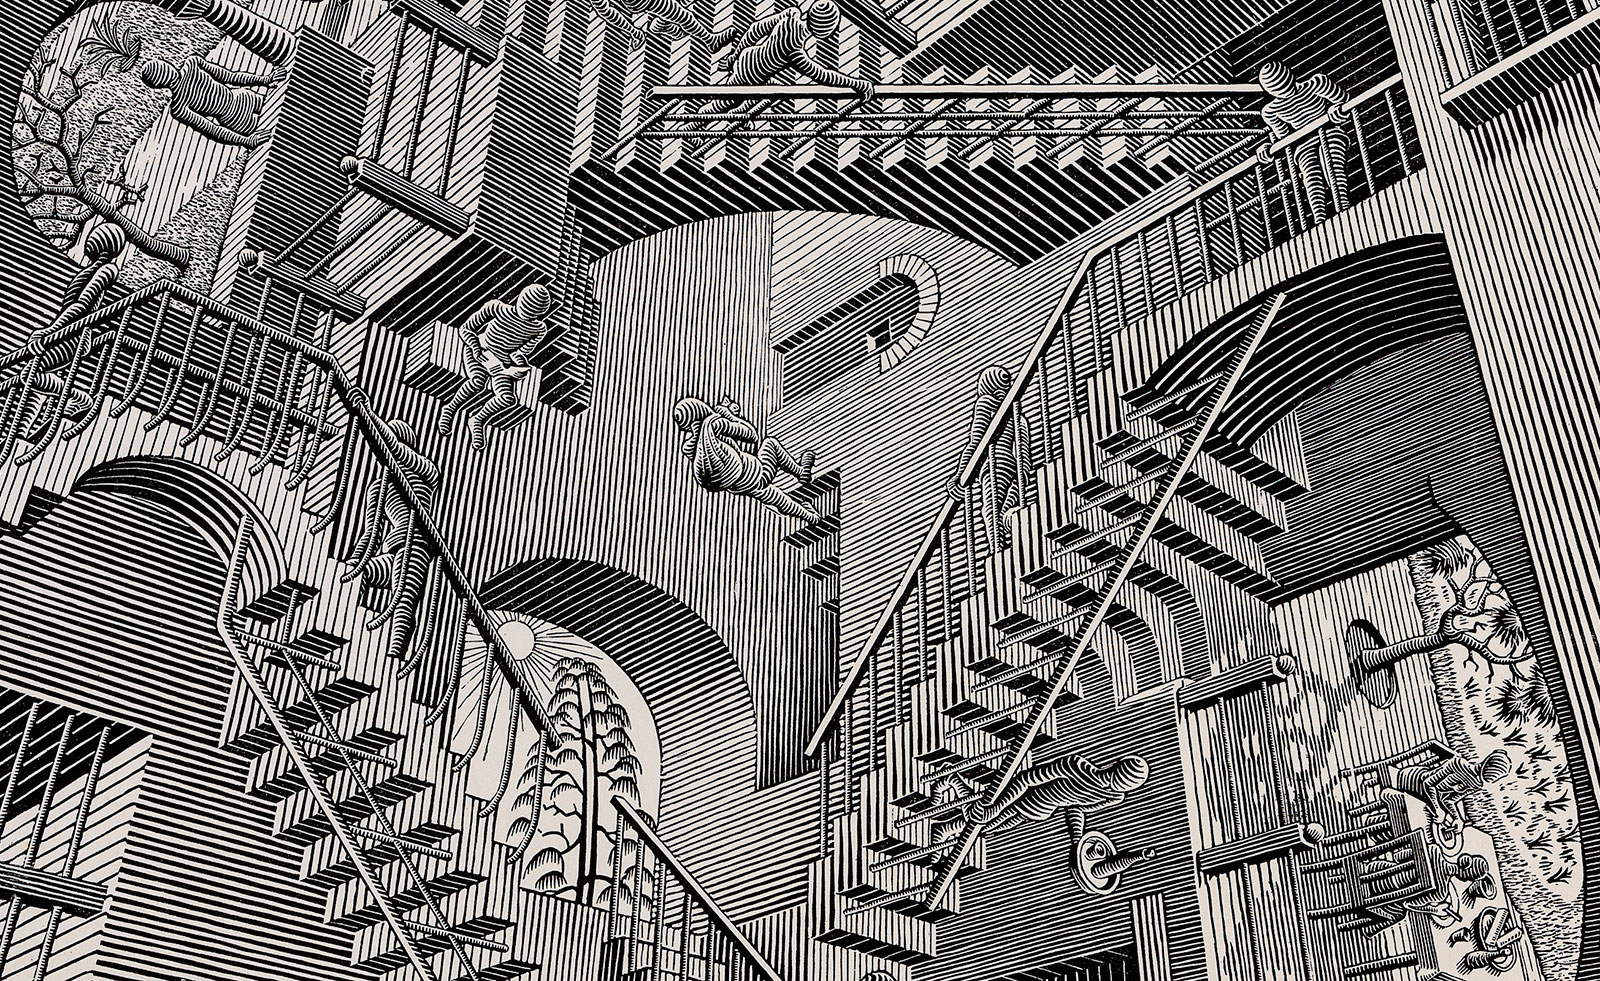
\includegraphics[width=\textwidth]{relativity.jpg}
	\caption{\textit{Relativity} by M.C. Escher, a complex image consisting of various sinusoidal patterns.}
	\label{fig:relativity}
\end{figure}

\begin{figure}[htb]
	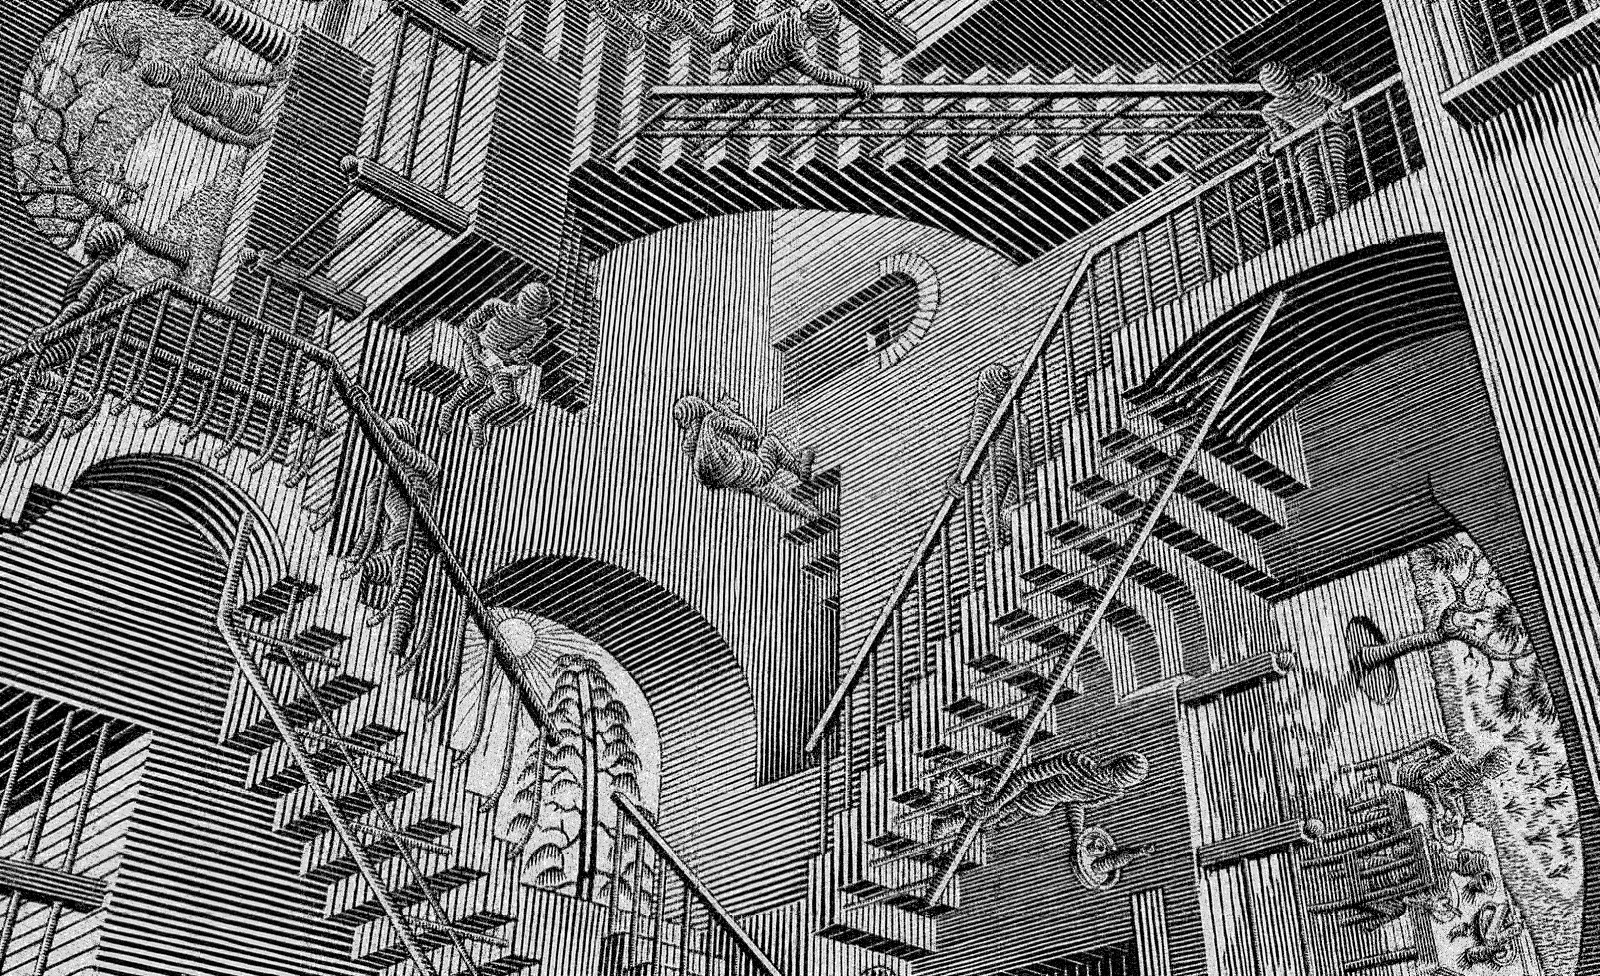
\includegraphics[width=\textwidth]{relativity-recovered.png}
	\caption{Reconstructed \textit{Relativity} from 50\% of samples from each patch.}
	\label{fig:relativity-recovered}
\end{figure}

\begin{figure}[htb]
	\centering
	\begin{subfigure}{\textwidth}
		\centering
		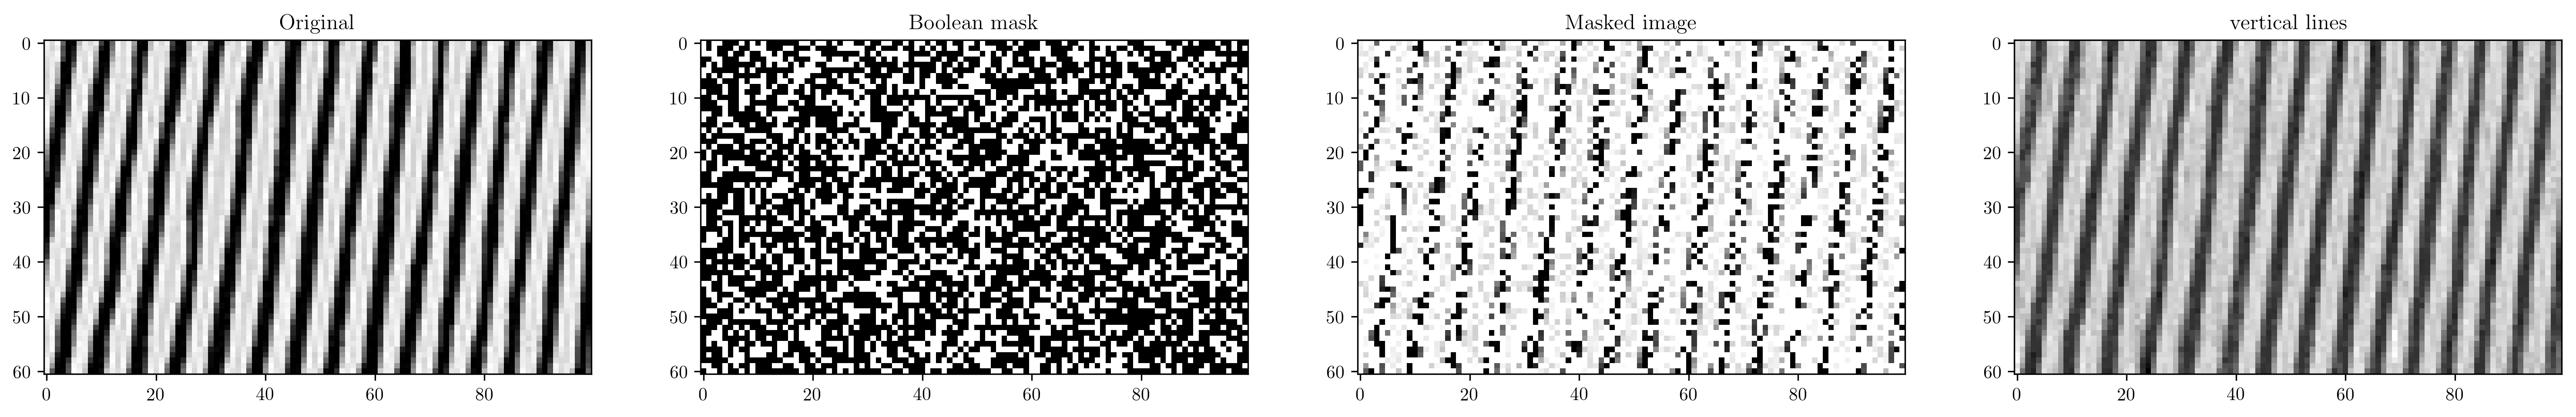
\includegraphics[width=\textwidth]{relativity-vert40.png}
		\caption{Dominant vertical}
		\label{fig:relativity-vert40}
	\end{subfigure}
	\begin{subfigure}{\textwidth}
		\centering
		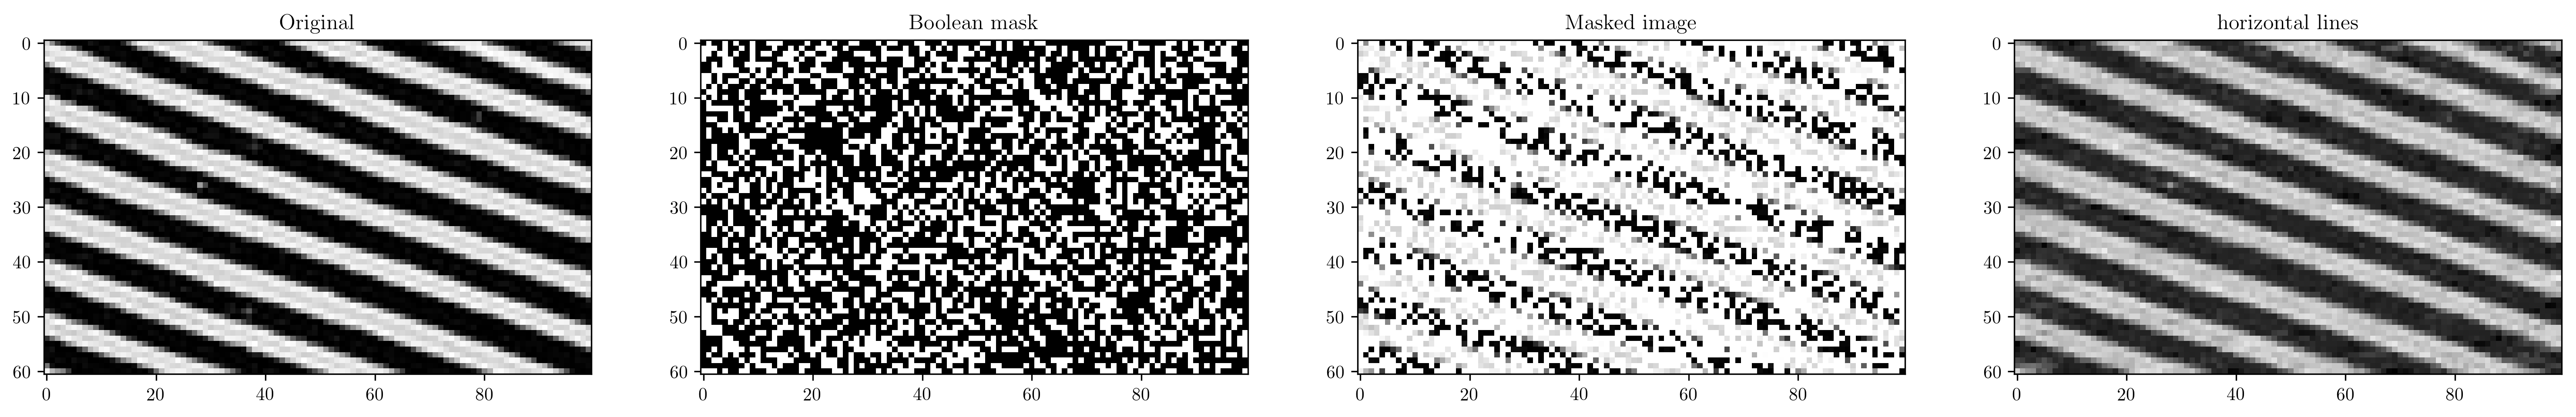
\includegraphics[width=\textwidth]{relativity-horiz40.png}
		\caption{Dominant horizontal}
		\label{fig:relativity-horiz40}
	\end{subfigure}
	\begin{subfigure}{\textwidth}
		\centering
		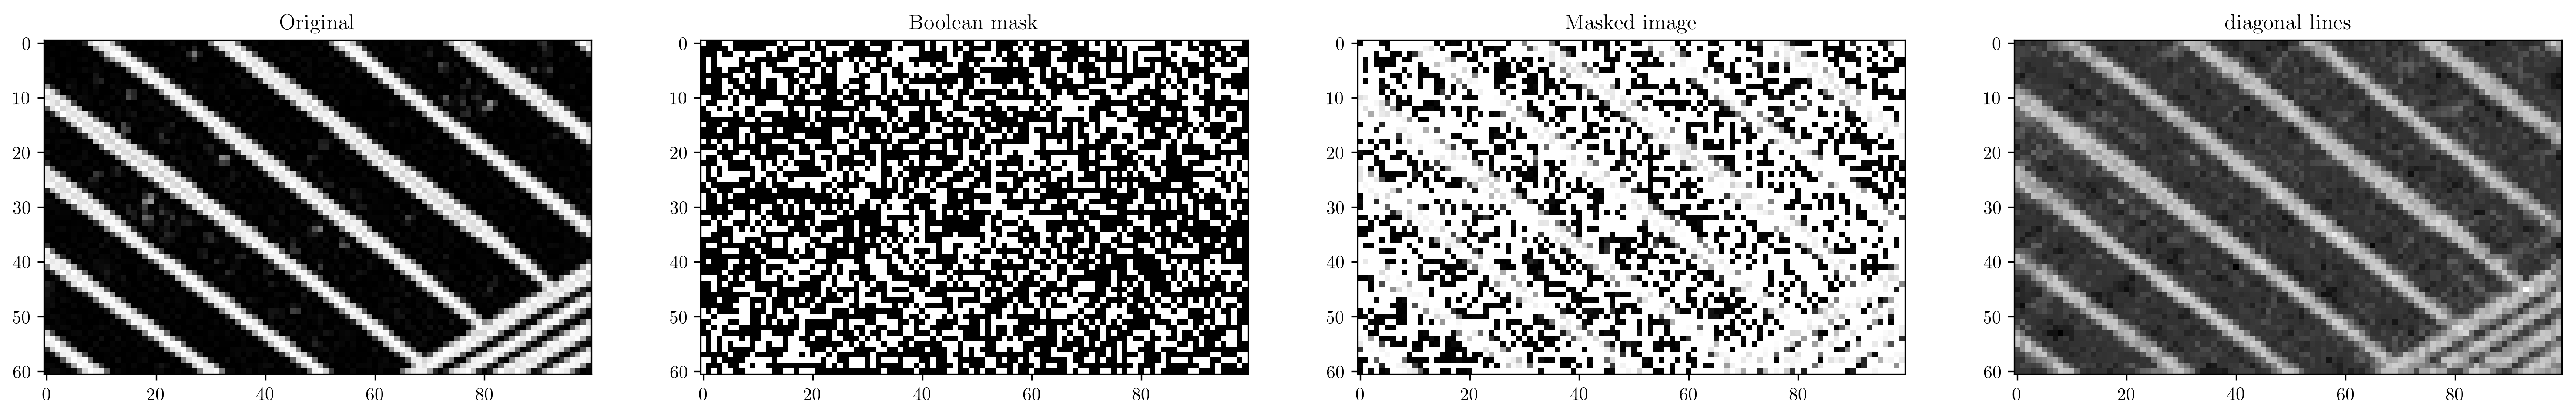
\includegraphics[width=\textwidth]{relativity-diag40.png}
		\caption{Dominant diagonal}
		\label{fig:relativity-diag40}
	\end{subfigure}
	\begin{subfigure}{\textwidth}
		\centering
		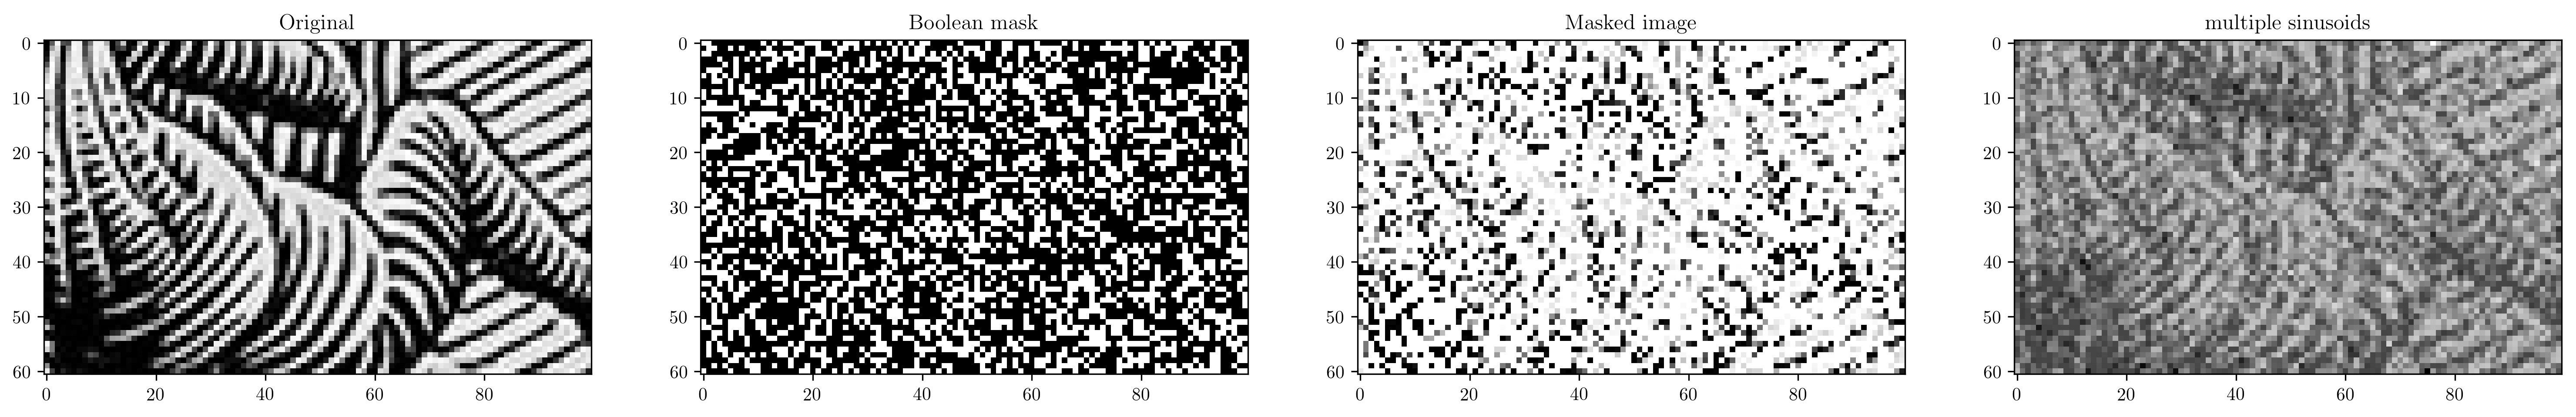
\includegraphics[width=\textwidth]{relativity-mult40.png}
		\caption{Multiple dominant sinusoids}
		\label{fig:relativity-mult40}
	\end{subfigure}
	\begin{subfigure}{\textwidth}
		\centering
		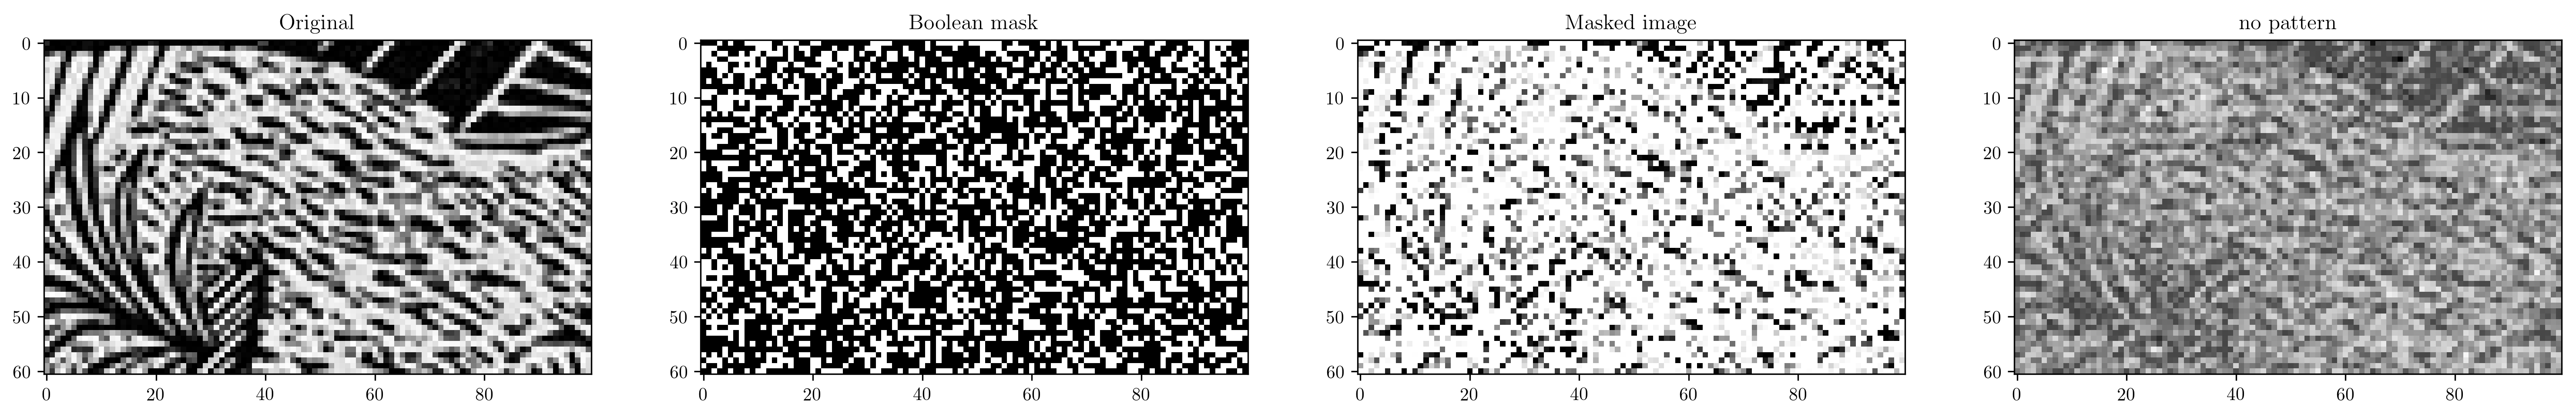
\includegraphics[width=\textwidth]{relativity-high40.png}
		\caption{No dominant pattern}
		\label{fig:relativity-high40}
	\end{subfigure}
	\caption{Extracted and reconstructed patches from \textit{Relativity} using 40\% of samples.}
	\label{fig:relativity-dominant-slices}
\end{figure}


\section{Simultaneous compression \& encryption}
Because of the way compressively sampled images are coded with the sensing matrix, the use of CS as an encryption algorithm arises naturally. Consider the logistic map

\begin{equation}\label{eq:logistic-map}
x_{n+1} = r x_n \qty(1 - x_n)
\end{equation}

\noindent which is often used as an archetypal example of deterministic chaotic behavior for values of $r \in [3.57, 4)$. In this regime, the sequences produced by varying the initial parameter $x_0$ rapidly diverge from each other. Thus, this can become an encryption system by treating the parameters $r$ and $x_0$ as an encryption key set, and \eqref{eq:logistic-map} as the hash function. One key set is then needed for each signal dimension. Thus, two key sets are needed for grayscale image applications (six, in the case of an RGB image and a unique key set for each color channel). 

\subsection{Methodology}
\label{ssec:image-encrypt-metho}
The construction of the sensing matrix $\bm\Phi$ differs from the general workflow, and is as follows:

\begin{enumerate}
	\item From \eqref{eq:logistic-map}, generate a sequence of length $2m$ with the initial key pair $r_1$ and $x_{01}$. Discard the first $n$ elements to avoid the transient response and store the latter $n$ elements as a sequence $\vec{s}$.
	\item Explicitly generate the index sequence of $\vec{s}$ and store it as sequence $\vec{p} = \qty[0, 1, ..., m-1]$.
	\item Sort $\vec{p}$ according to ascending values of $\vec{s}$.
	\item Generate the first sensing matrix $\bm\Phi_1$ by extracting and stacking rows of a Hadamard matrix $\vec{H}$ of order $N$ indexed by the first $m$ elements of $\vec{p}$, i.e.,
	\begin{equation}\label{eq:construct-hadamard}
	\bm\Phi_1 = \mqty[
	\vec{H}_{p_1} & \vec{H}_{p_2} & \cdots & \vec{H}_{p_m}
	]^\top
	\end{equation}
	\noindent where $\vec{H}_{p_i}$ denotes the $p_i$th row vector of $\vec{H}$.
	\item Any other sensing matrices can be constructed in the same way.
\end{enumerate}

The usage of a Hadamard matrix implies that the image must first be reshaped to have dimensions that are integer multiples of 4. The original image is first reshaped to $256 \times 256$ pixels, and is sparsified by transforming it to the DCT domain. The desired compressed dimension is set to $m = 192$, corresponding to a compression ratio of 75\%, and the keys are set to values of $r_1 = r_2 = 3.99$, $x_{01} = 0.11$, and $x_{02} = 0.24$.

\subsection{Results \& discussion}
\label{ssec:image-encrypt-rnd}
Figure~\ref{fig:encryption} shows the application of this to the Lena test image. Visual inspection of the encrypted representation shows horizontal and vertical bands distributed throughout the representation space, and is indicative that a simple inverse Fourier transform will not recover any meaningful information. Assuming that the receiver knows the encryption scheme, recovery of the original message is successful if the same keys $r_1, r_2, x_{01}, x_{02}$ as the encryption stage are used, which will allow the receiver to construct the exact same sensing matrices $\bm\Phi_1, \bm\Phi_2$ and perform the inverse operation on the encrypted message. In the decrypted image, encryption artifacts can be observed, as indicated by some visible banding, but is nonetheless recognizable; evaluation of the MSE and SSIM yields values of 0.02 and 0.82, respectively.

\begin{figure}[htb]
	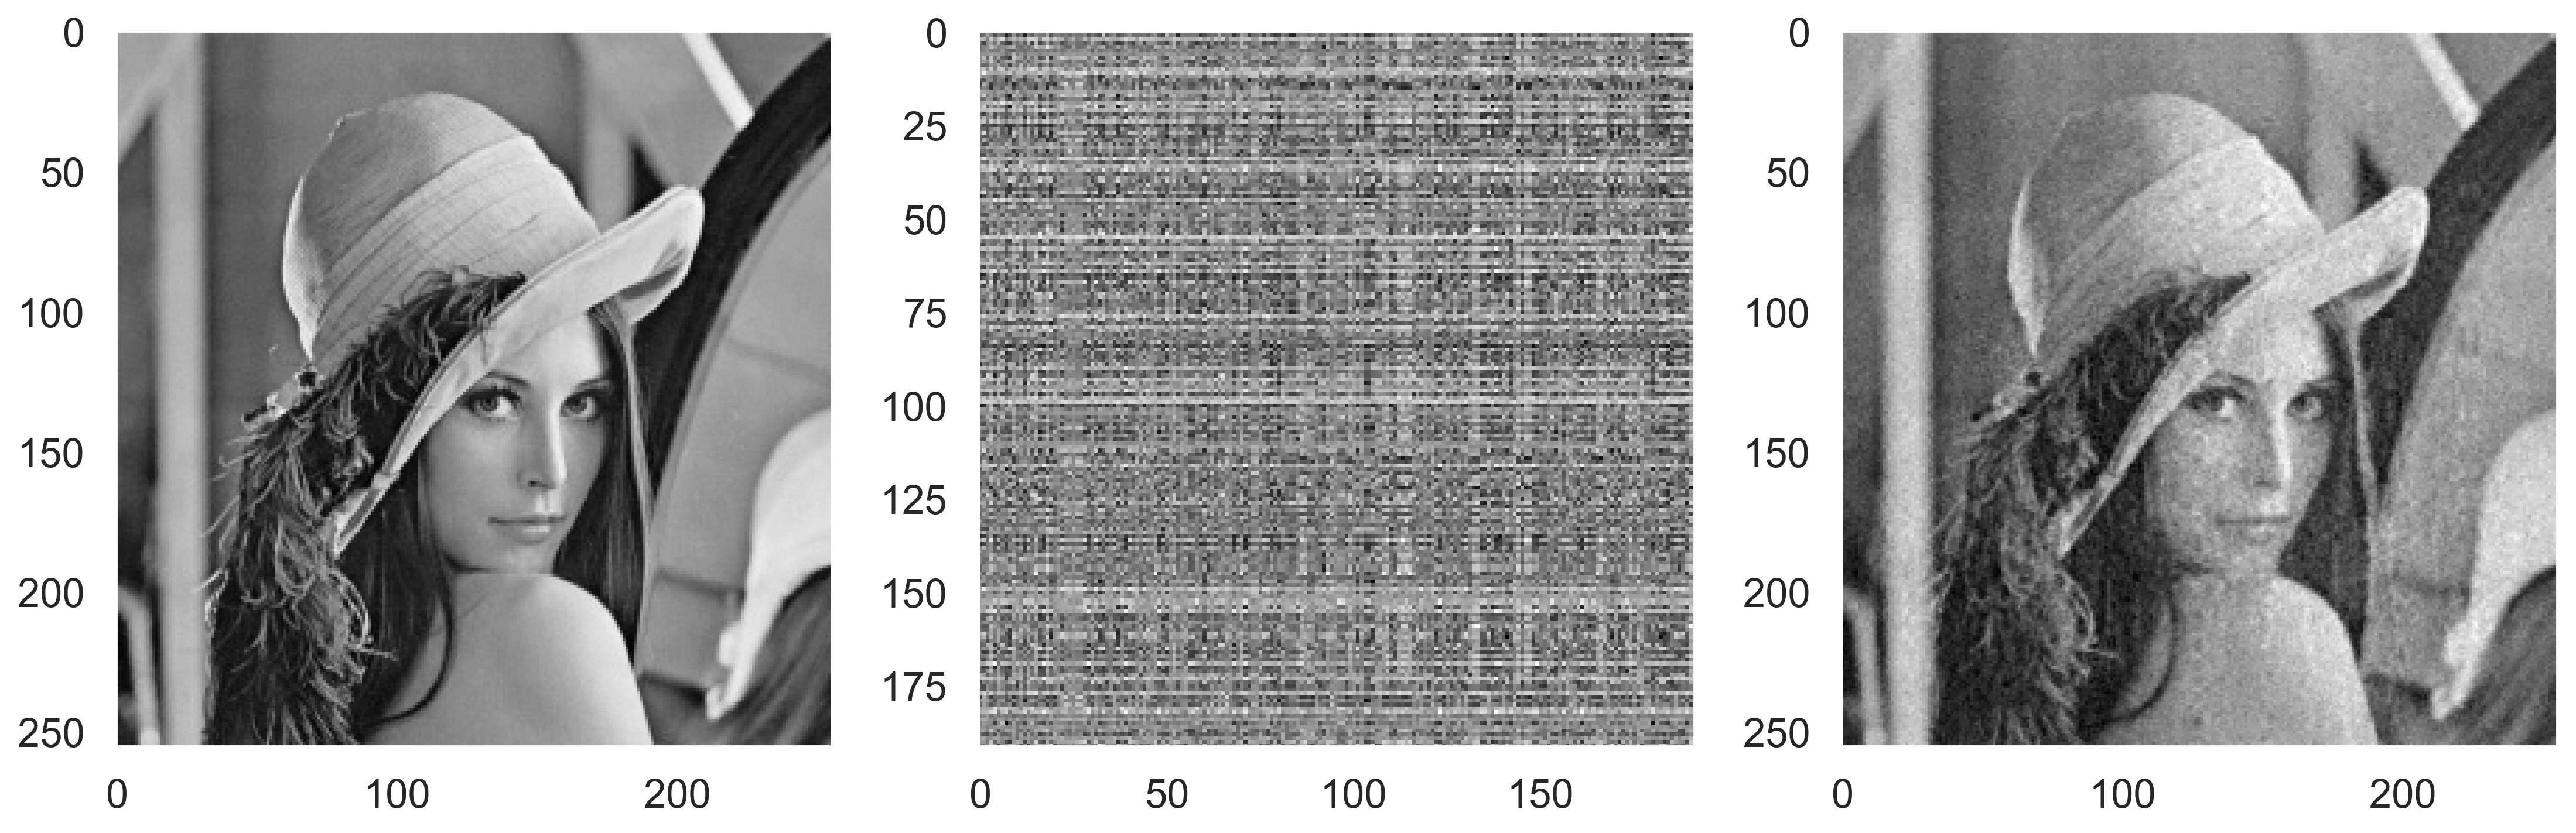
\includegraphics[width=\textwidth]{encryption.png}
	\caption{Simultaneous compression and encryption achieved with compressive sensing: original image (left), encrypted image (middle), and decrypted/reconstructed image (right).}
	\label{fig:encryption}
\end{figure}

\subsection{Correlation analysis}
\label{ssec:image-encrypt-correlation}
Correlation is a statistical measure of obtaining useful information from a given signal by analyzing adjacent pixels. The correlation coefficients can be obtained by

\begin{equation}
\label{eq:correlation-coeff}
C = \frac{\sum_{i=1}^N (x_i - \ev{\vec{x}}) (y_i - \ev{\vec{y}})}{\sqrt{\sum_{i=1}^N (x_i - \ev{\vec{x}})^2 \sum_{i=1}^N (y_i - \ev{\vec{y}})^2}}
\end{equation}

\noindent where $\vec{x}$ and $\vec{y}$ are the original and encrypted signals, respectively. For the purposes of encryption, a correlation coefficient closer to 0 is better. Table~\ref{tab:correlation} shows the computed correlations for the original and encrypted Lena images in the horizontal, vertical, and diagonal directions. The correlation of the encrypted signal is much lower than that of the original, which means that a potential attacker cannot gain any useful information by employing statistical analyses.

\begin{table}
	\centering
	\caption{Correlation coefficients of test Lena image.}
	\label{tab:correlation}
	\begin{tabular}{rrrr}
		\toprule
		& horizontal & vertical & diagonal \\
		\midrule
		original & 0.94 & 0.97 & 0.91 \\
		encrypted & 0.42 & 0.02 & $-0.05$ \\
		\bottomrule
	\end{tabular}
\end{table}


\subsection{Key sensitivity analysis}
\label{ssec:image-encrypt-keysensitivity}
With the knowledge that the hash function $\eqref{eq:logistic-map}$ is chaotic, the sensitivity of the encryption system to the keys can be tested by perturbing the initial keys with small values. Figure~\ref{fig:wrong-decryption} shows the decryption results when all the correct keys are used, except for $x_{01}$, which is perturbed by a tiny value $\approx 10^{-15}$ (third image), and similarly when the correct $x_{01}$ is used but $x_{02}$ is perturbed by the same amount (last image).

\begin{figure}[htb]
	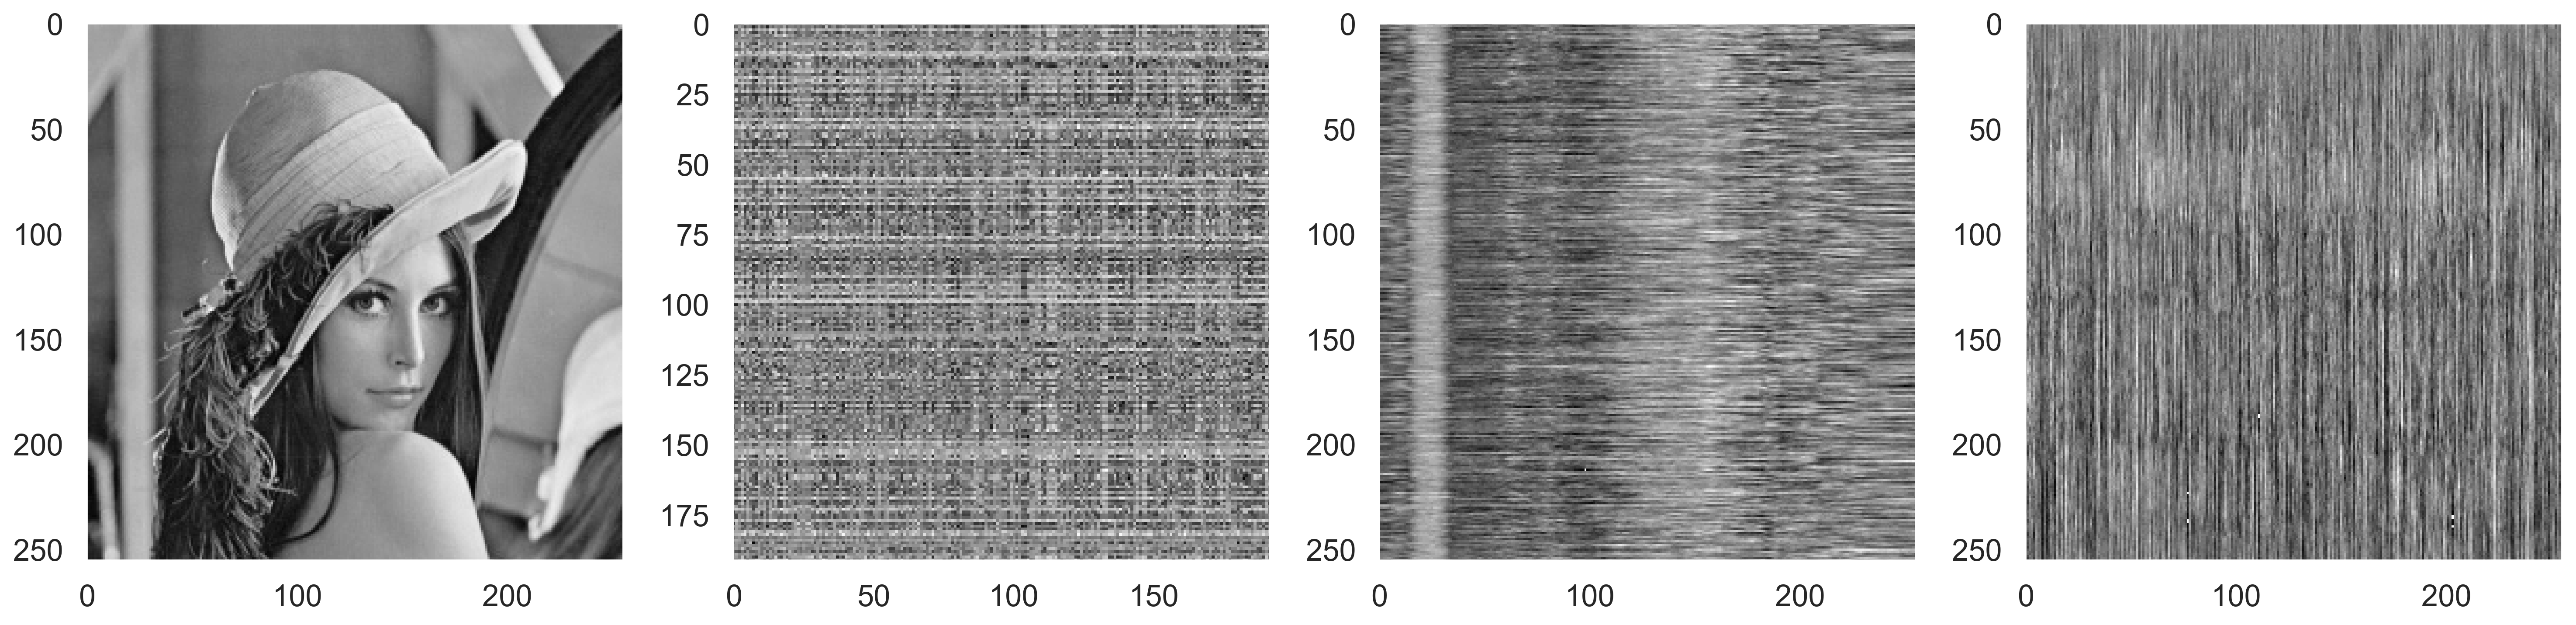
\includegraphics[width=\textwidth]{wrong_decrypt.png}
	\caption{Test image Lena (first) with the encrypted representation (second), the decryption result when the correct keys are used but $x_{01}$ is perturbed by a value of $10^{-15}$ (third), and the decryption result when the correct keys are used but $x_{02}$ is perturbed by a value of $10^{-15}$.}
	\label{fig:wrong-decryption}
\end{figure}

Additionally, Fig.~\ref{fig:perturb-mse} shows the MSE curves evaluated by varying values of the perturbation $\Delta x_{01}$ and $\Delta x_{02}$. Perturbations are generated as 100 equally-spaced values in the range $\pm 10^{-14}$, plus zero. This specific value was chosen because the resolution of a double precision floating point number in Python on a 64-bit CPU architecture is $10^{-16}$. The MSE generally oscillates at some high value, and exhibits a sharp dip when the MSE is evaluated for the correct keys ($\Delta x_0 = 0$). The same is done for Fig.~\ref{fig:perturb-ssim}, which shows the SSIM curves. Similarly, values oscillate at a low value, corresponding to recovered signals with no meaningful data. Maximum SSIM of 0.83 is achieved only for the correct keys. This shows that brute force attacks are intractable against this kind of encryption system.

\begin{figure}[htb]
	\centering
	\begin{subfigure}{0.49\textwidth}
		\centering
		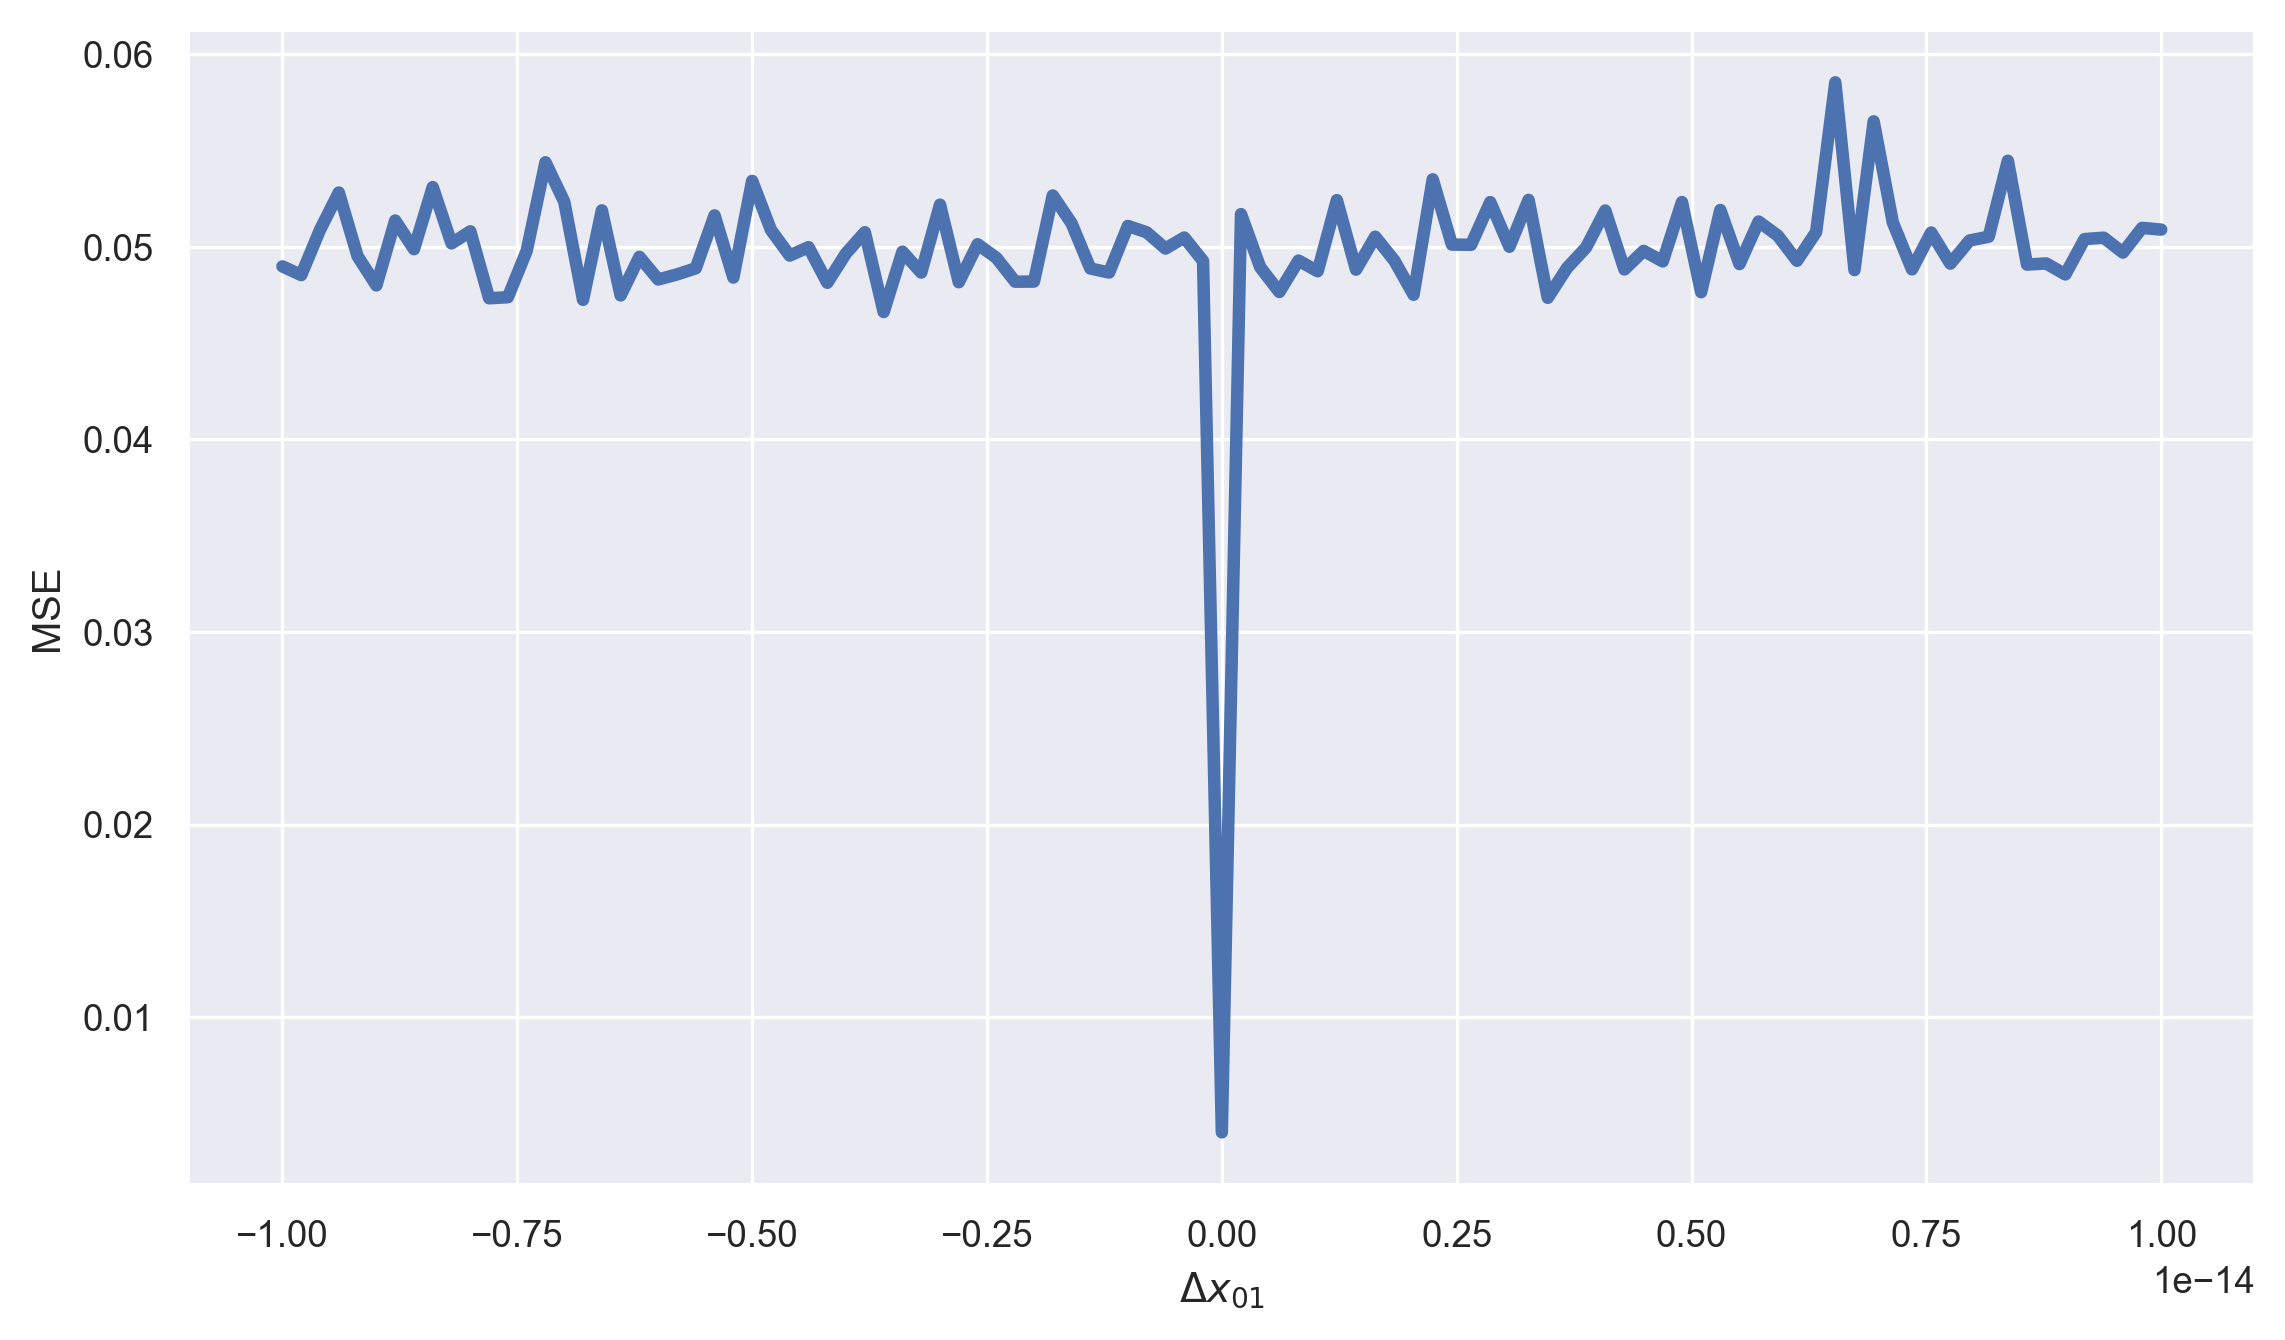
\includegraphics[width=\textwidth]{mse-x01.png}
		\caption{Perturbation of $\Delta x_{01}$}
		\label{fig:perturb-mse-x01}
	\end{subfigure} 
	\begin{subfigure}{0.49\textwidth}
		\centering
		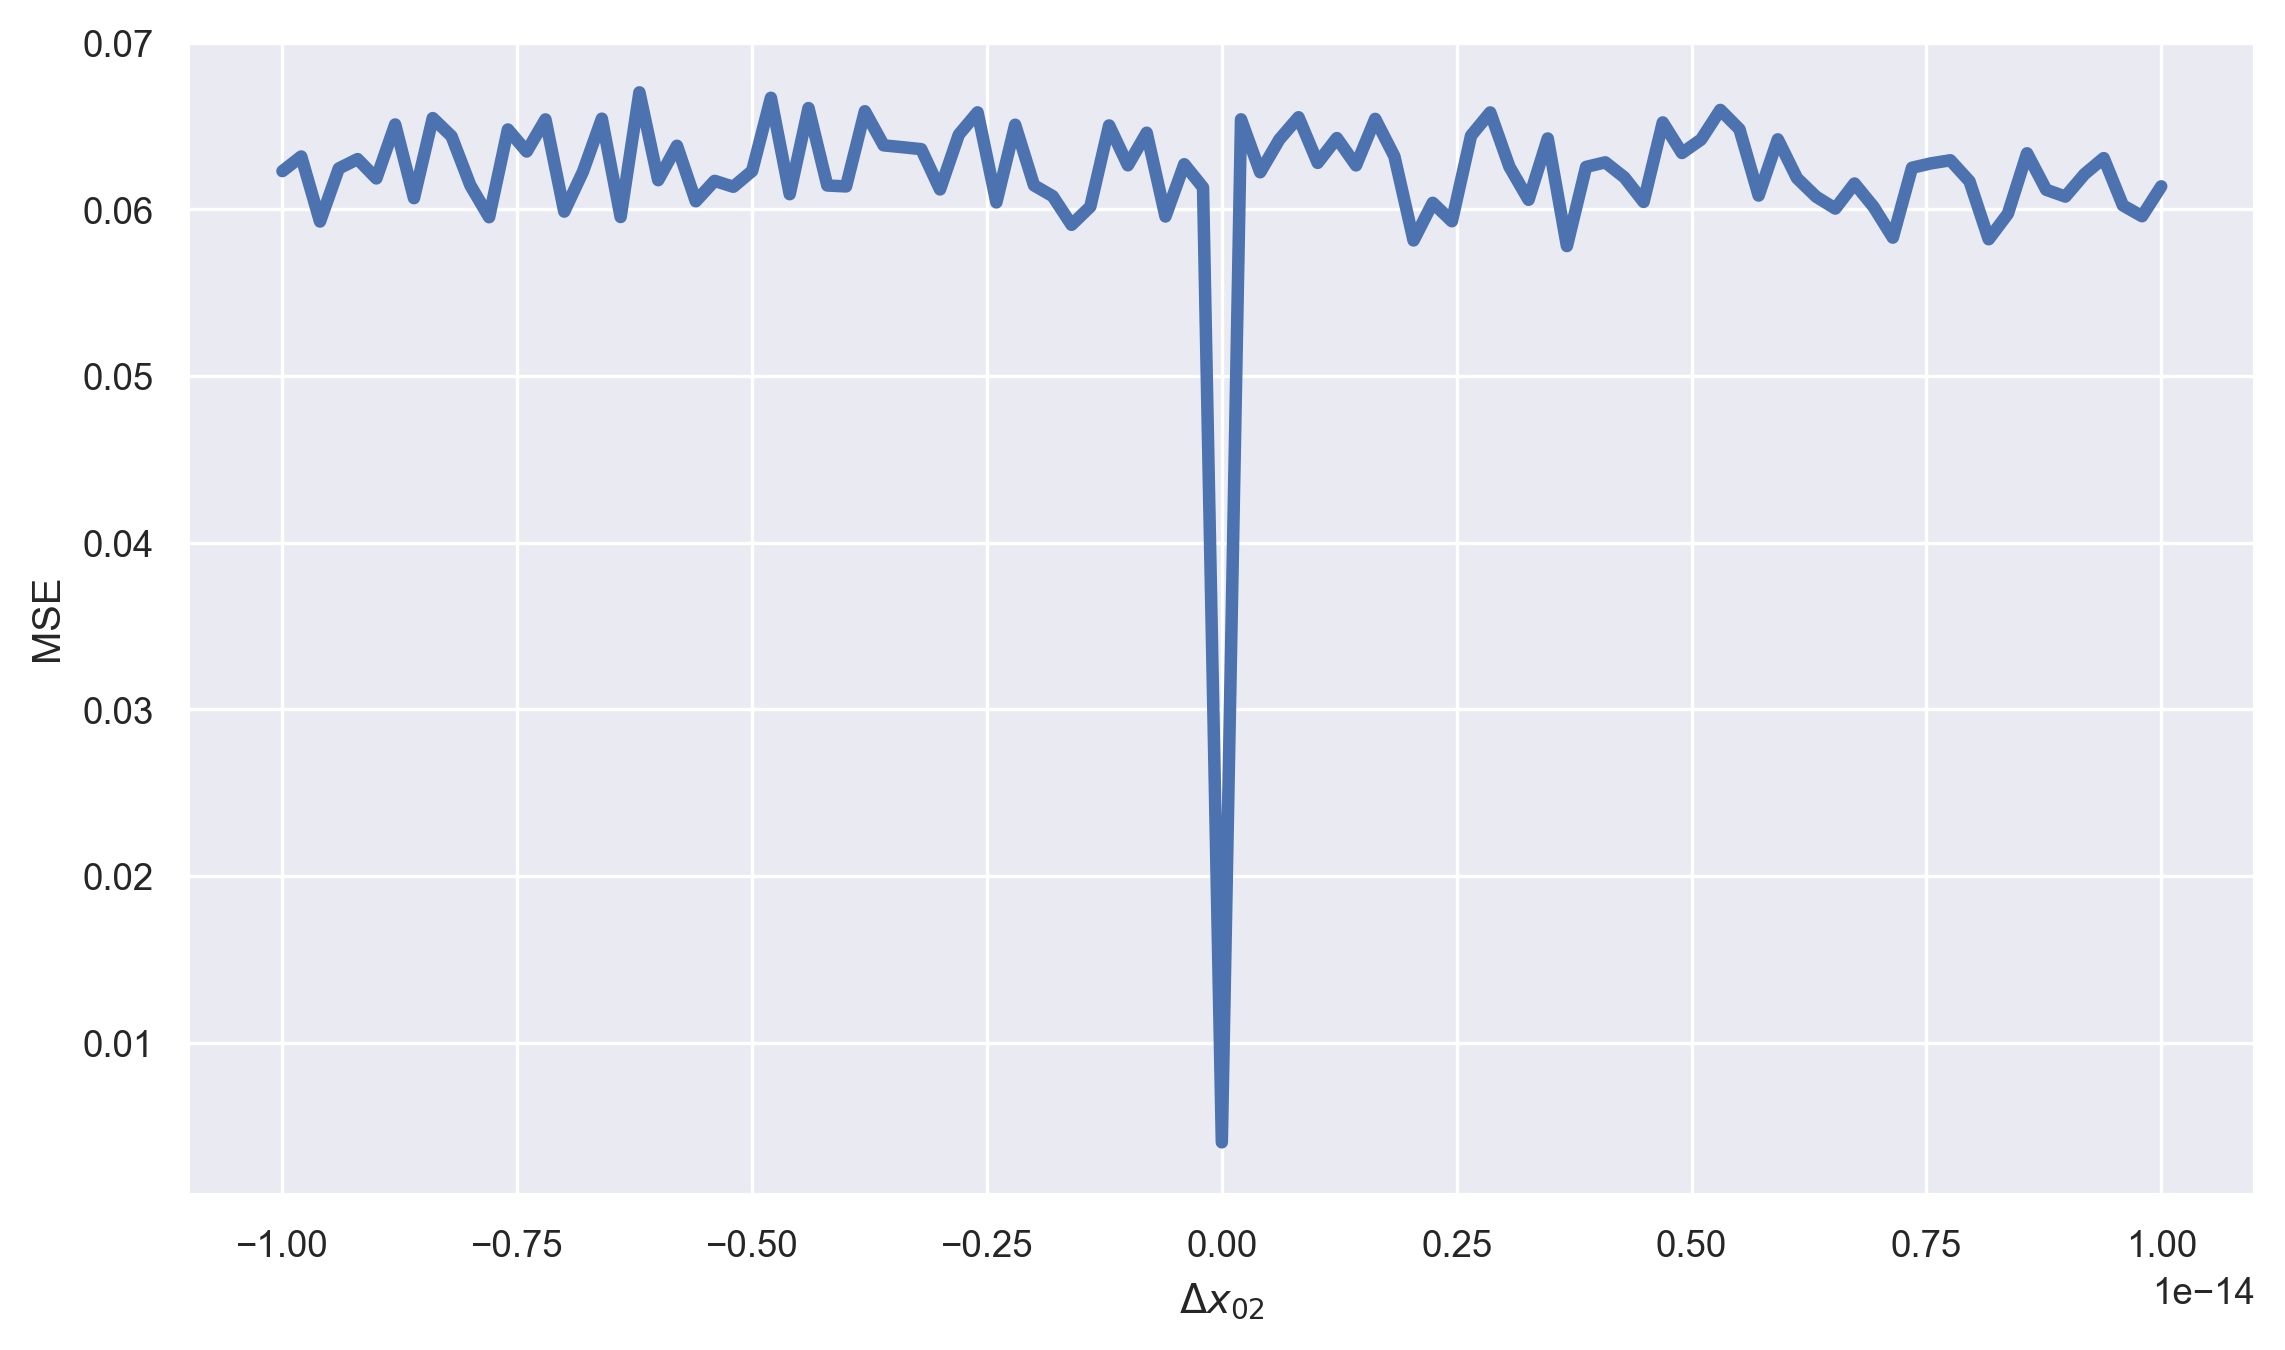
\includegraphics[width=\textwidth]{mse-x02.png}
		\caption{Perturbation of $\Delta x_{02}$}
		\label{fig:perturb-mse-x02}
	\end{subfigure}
	\caption{MSE curves resulting from evaluation of reconstruction error for tiny perturbations in the initial values $\Delta x_{01}$ and $\Delta x_{02}$.}
	\label{fig:perturb-mse}
\end{figure}

\begin{figure}[htb]
	\centering
	\begin{subfigure}{0.49\textwidth}
		\centering
		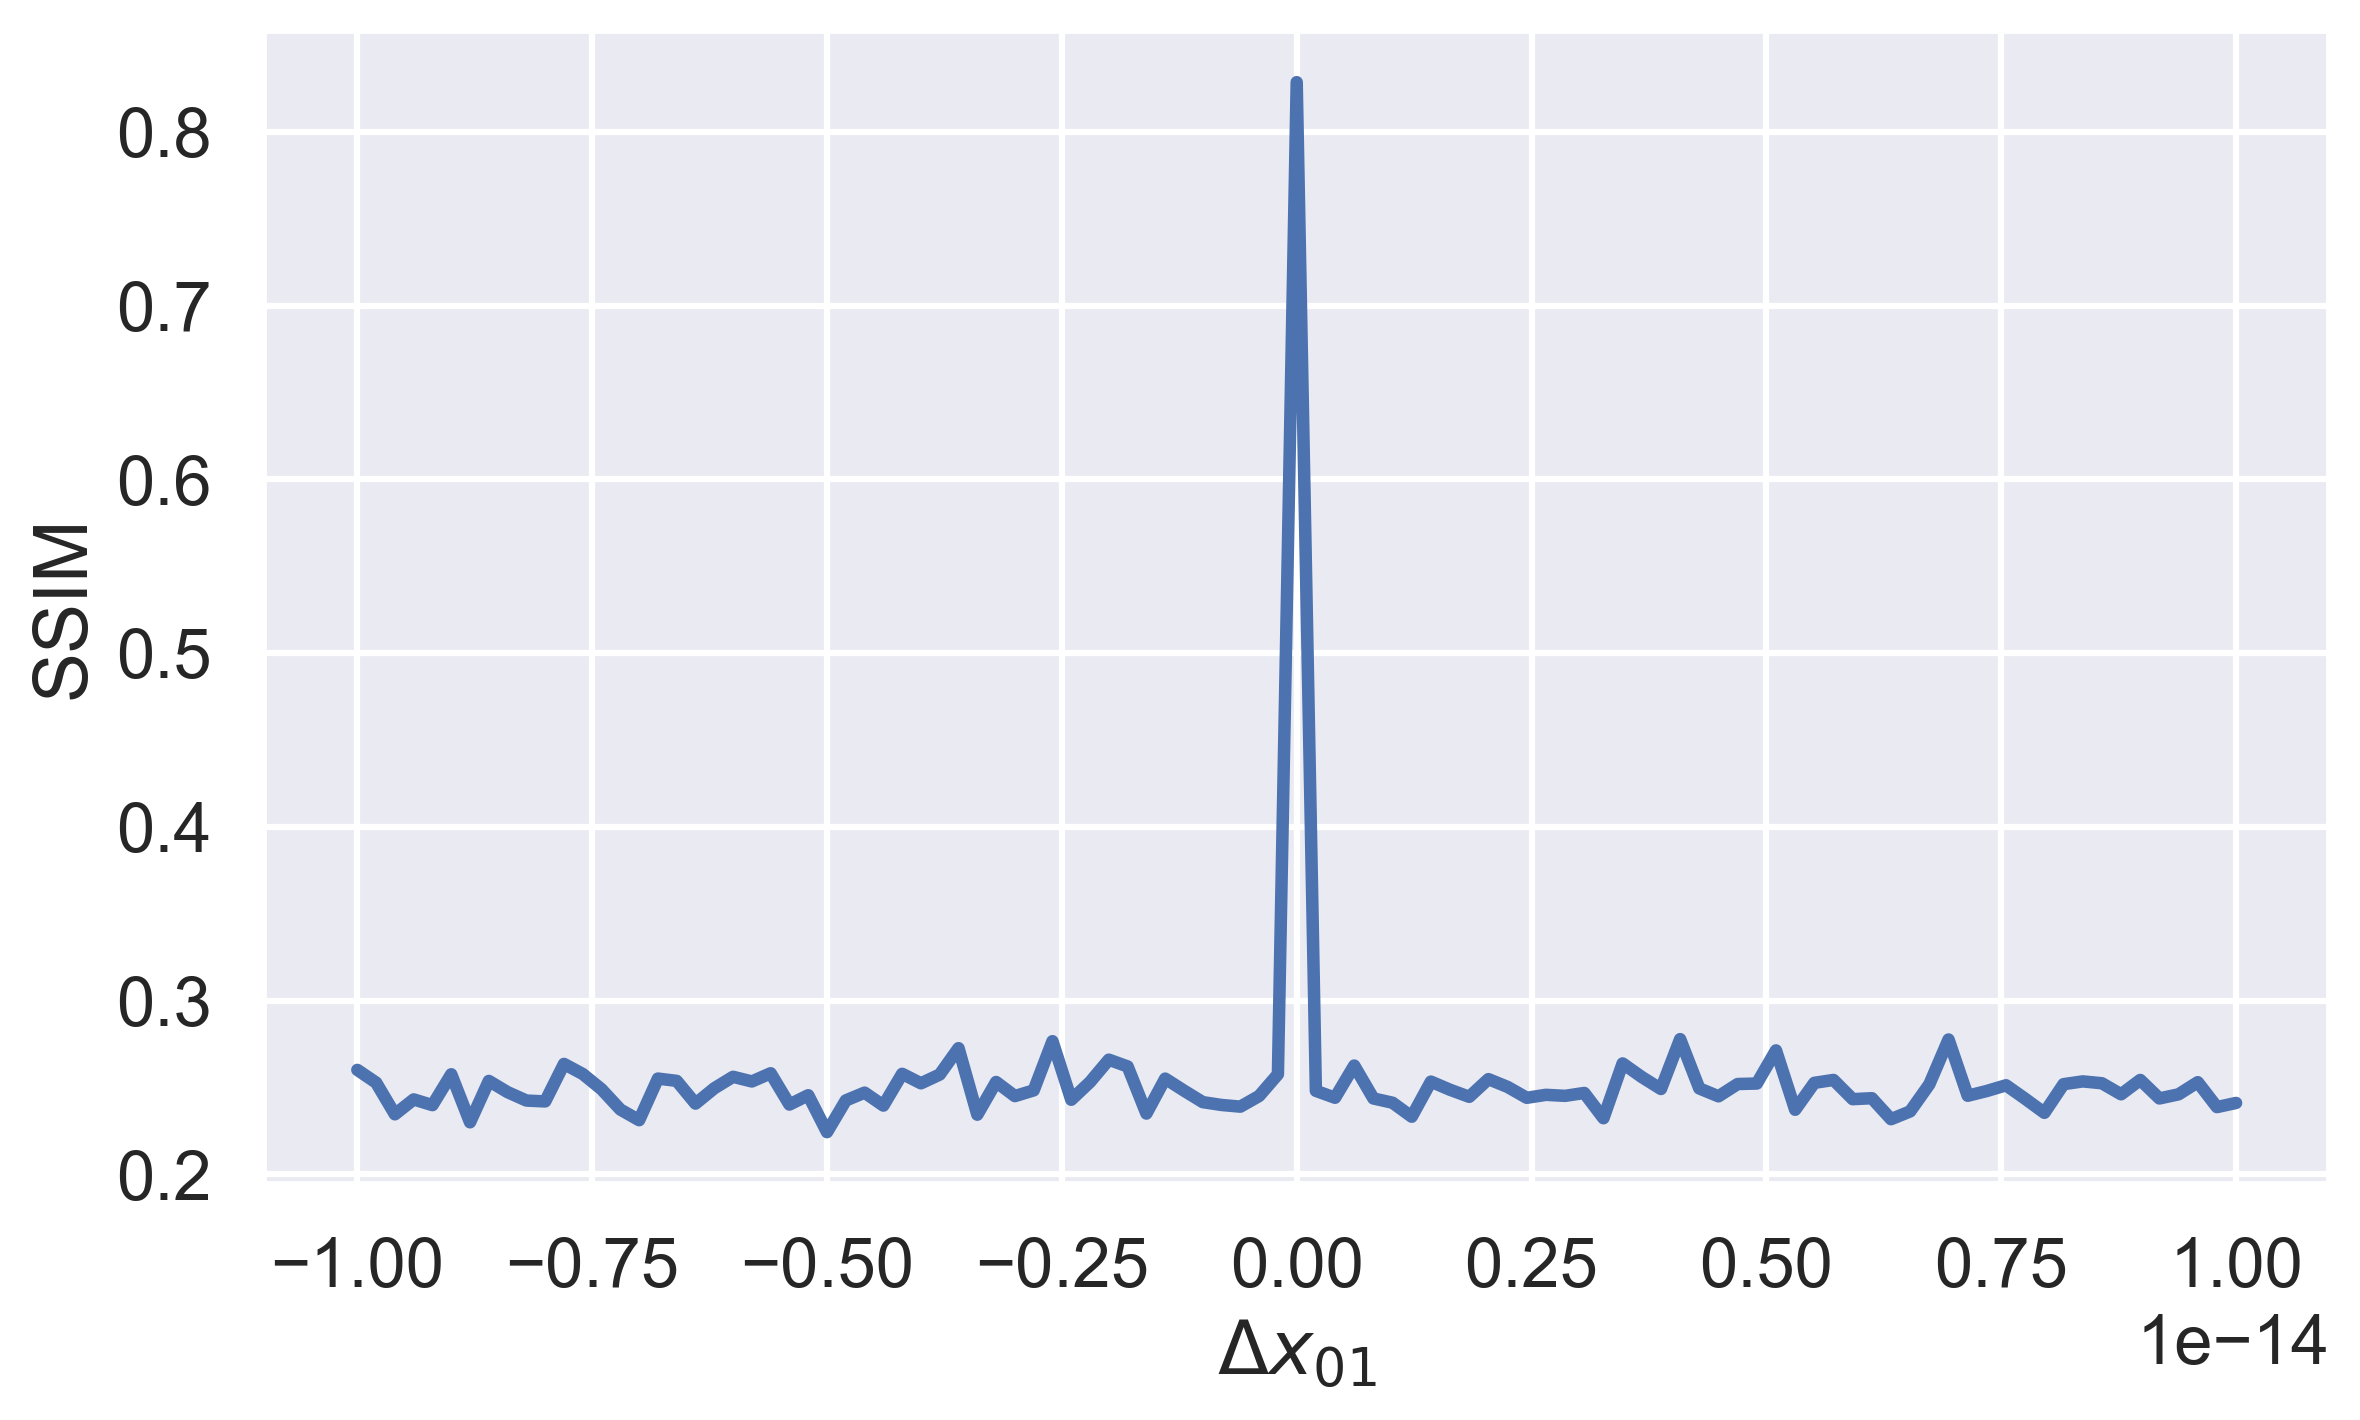
\includegraphics[width=\textwidth]{ssim-x01.png}
		\caption{Perturbation of $\Delta x_{01}$}
		\label{fig:perturb-ssim-x01}
	\end{subfigure} 
	\begin{subfigure}{0.49\textwidth}
		\centering
		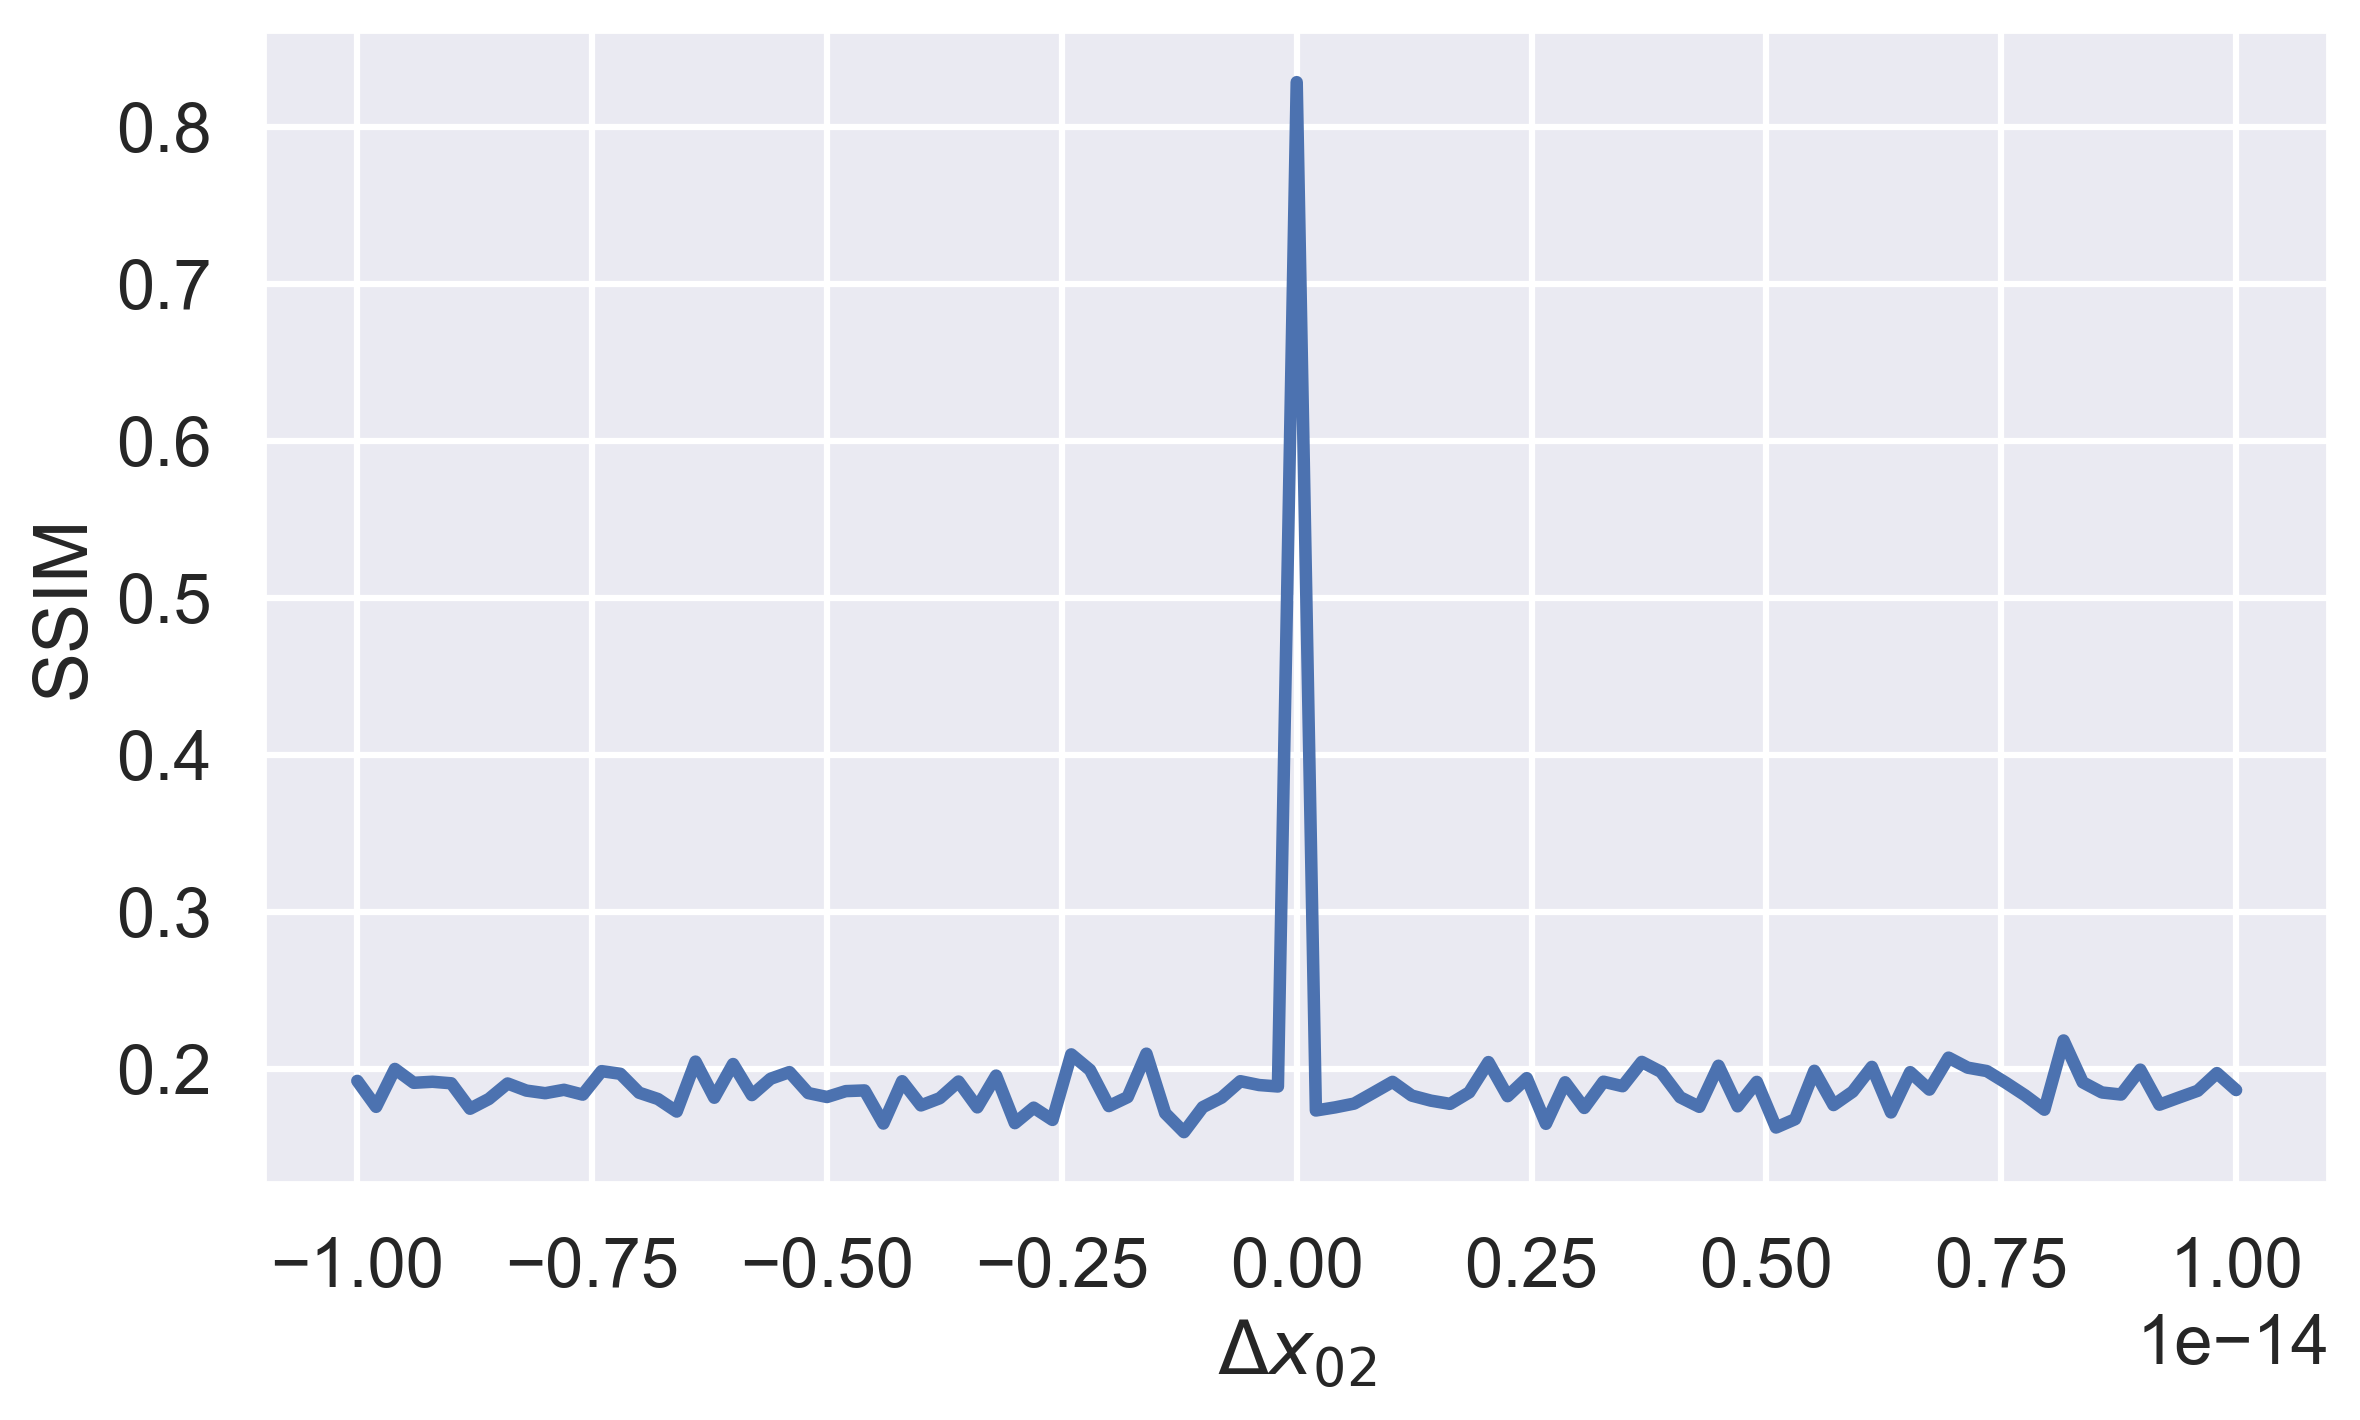
\includegraphics[width=\textwidth]{ssim-x02.png}
		\caption{Perturbation of $\Delta x_{02}$}
		\label{fig:perturb-ssim-x02}
	\end{subfigure}
	\caption{SSIM curves resulting from evaluation of reconstruction error for tiny perturbations in the initial values $\Delta x_{01}$ and $\Delta x_{02}$.}
	\label{fig:perturb-ssim}
\end{figure} %%could be results and discussions
% !TEX root =  main.tex
\chapter{Audio compressive sensing}
\label{chap:audio-cs}
In this chapter, I apply CS to audio signals. These type of signals act as the bridge to $N$-dimensional CS as they are one-dimensional when represented in the time domain, but are projected to higher dimensions when represented in another domain, such as the spectrogram/modulation domain. Unlike images, audio signals are more challenging to compressively sample. Due to their relatively higher information density, the effects of undersampling are easily observed.

\section{Test case: Sinusoid redux}
\label{sec:audio-sine}
In this test case, I recorded a guitar playing a single E$_4$ (330 Hz) note at the standard 44.1 kHz sampling rate for 4 seconds. Since the Nyquist rate of the actual signal is 660 Hz, the recording can be downsampled to a practical 8 kHz for processing. The signal waveform and frequency content is shown in Fig.~\ref{fig:guitar-original}. The base frequency is dominant in the frequency spectrum, and several harmonics can be observed. The goal here is to be able to recover the harmonics that have a frequency higher than the compressive sampling rate.

The compressed signal is shown in Fig.~\ref{fig:guitar-compressed}, which was compressively sampled with a quasi-frequency of 1000~Hz (1000 i.i.d.~random samples per second), corresponding to a 12.5\% compression ratio. The waveform envelope still resembles that of the original, but due to the random nature of sampling, the periodicity is not preserved, and is reflected in the seemingly random frequency content.

Following a similar process shown in Chapter \ref{chap:random-cs}, I chose DCT to be the sparse representation domain, and LASSO as the optimization algorithm. The reconstructed signal is shown in Fig.~\ref{fig:guitar-recovered}.For this case, I am concerned only with the frequency components that are recovered, and not so much with the magnitude. Thus, the reconstruction quality can be quantified using the cosine similarity

\begin{equation}
\label{eq:cossim}
\mathrm{similarity} = \cos\theta = \frac{\vec{x} \cdot \bm\hat{\vec{x}}}{\norm{\vec{x}}_2 \norm{\bm\hat{\vec{x}}}_2}
\end{equation}

\noindent which allows us to compare two signals' frequency content directly in the time domain. A cosine similarity value of 0.8 and above indicates acceptable quality; a value of 1.0 indicates perfect reconstruction.

\begin{figure}[htb]
	\centering
	\begin{subfigure}{\textwidth}
		\centering
		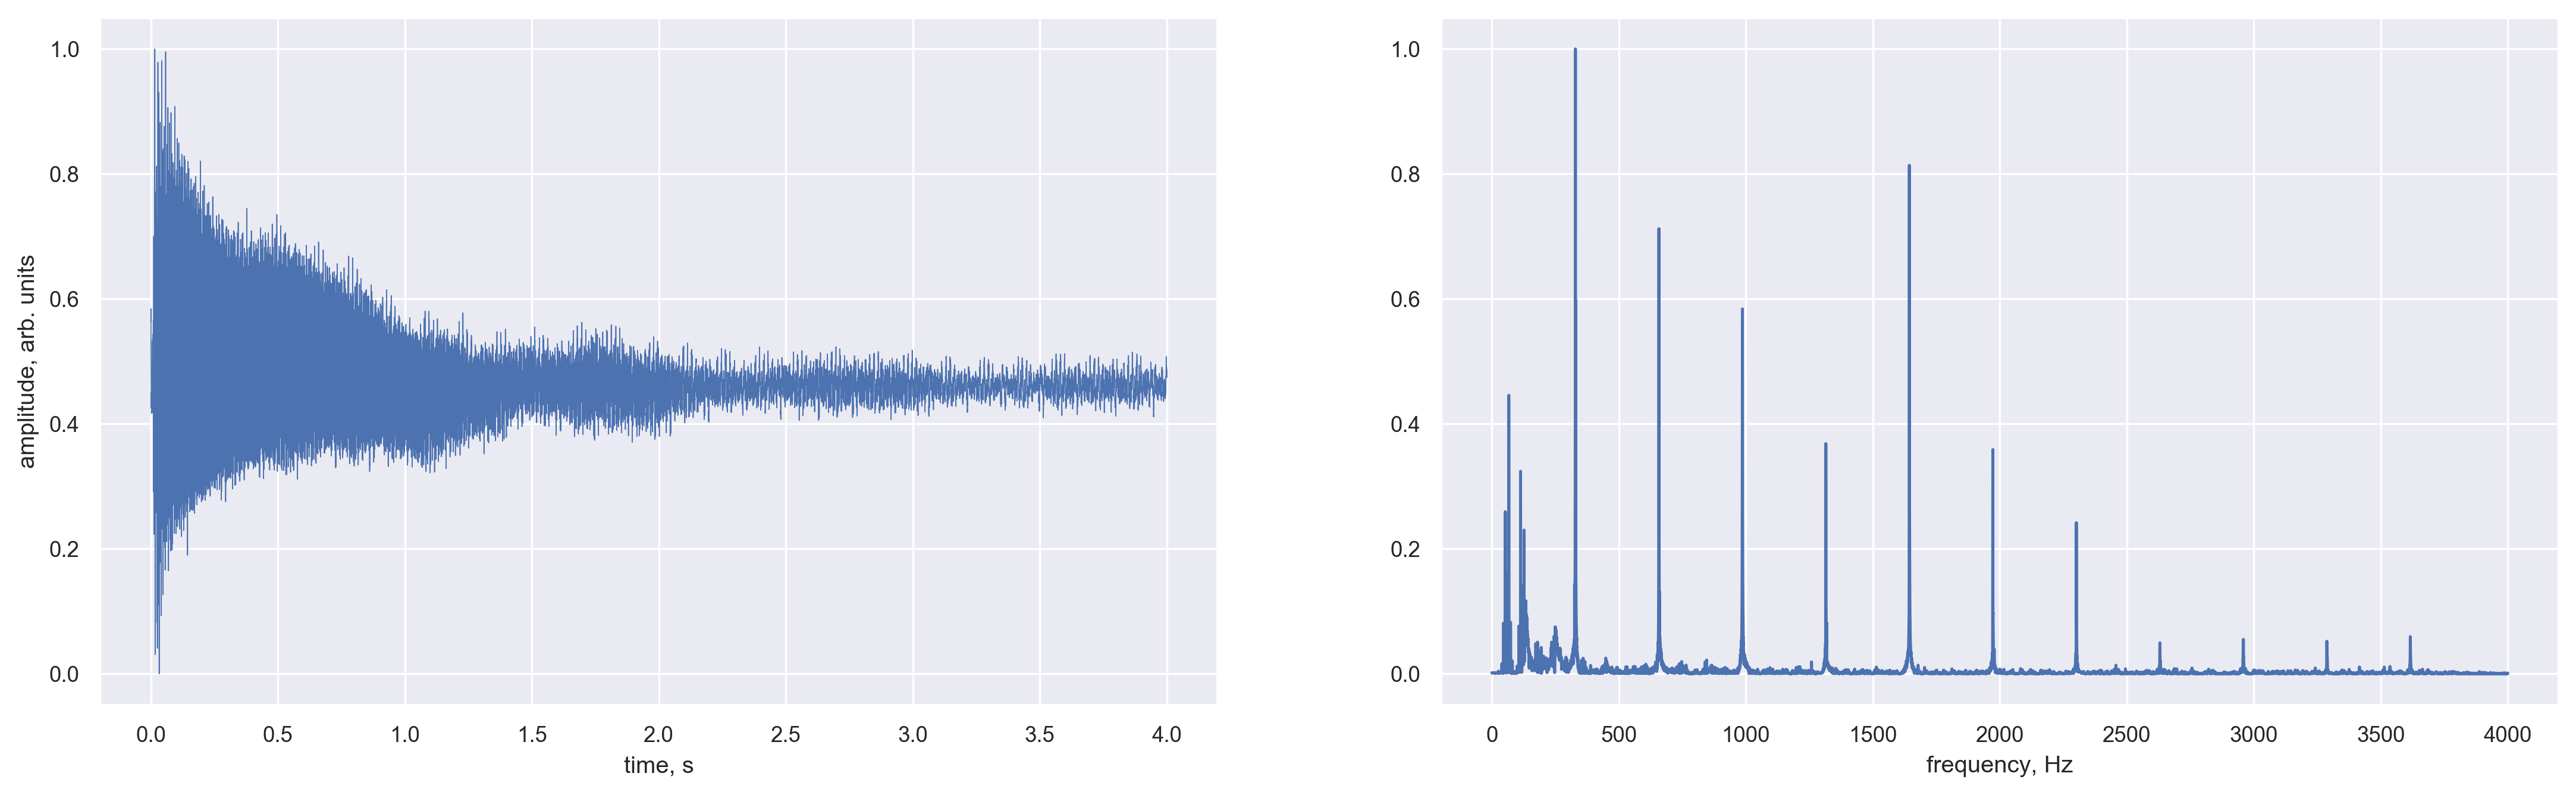
\includegraphics[width=\textwidth]{E1_orig.png}
		\caption{Original}
		\label{fig:guitar-original}
	\end{subfigure}
	\begin{subfigure}{\textwidth}
		\centering
		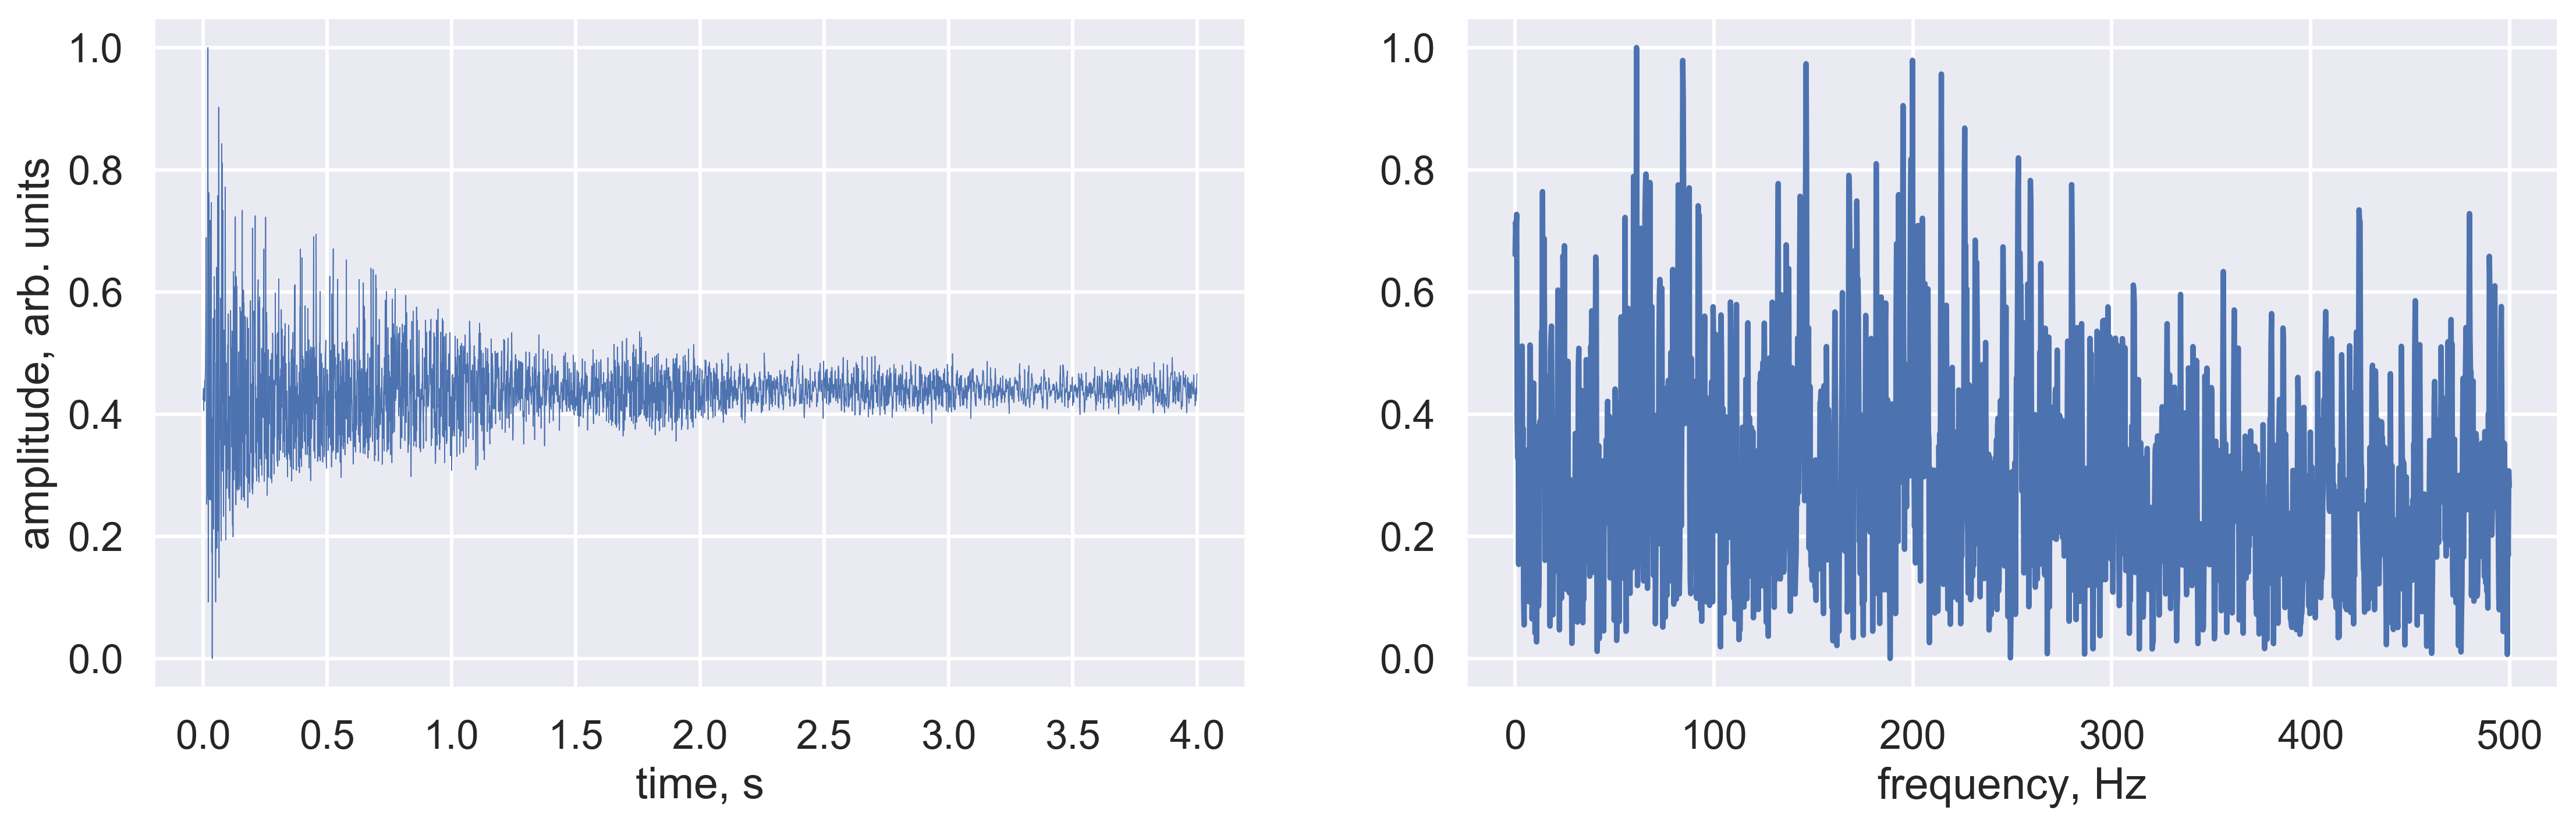
\includegraphics[width=\textwidth]{E1_comp.png}
		\caption{Compressed}
		\label{fig:guitar-compressed}
	\end{subfigure}
	\begin{subfigure}{\textwidth}
		\centering
		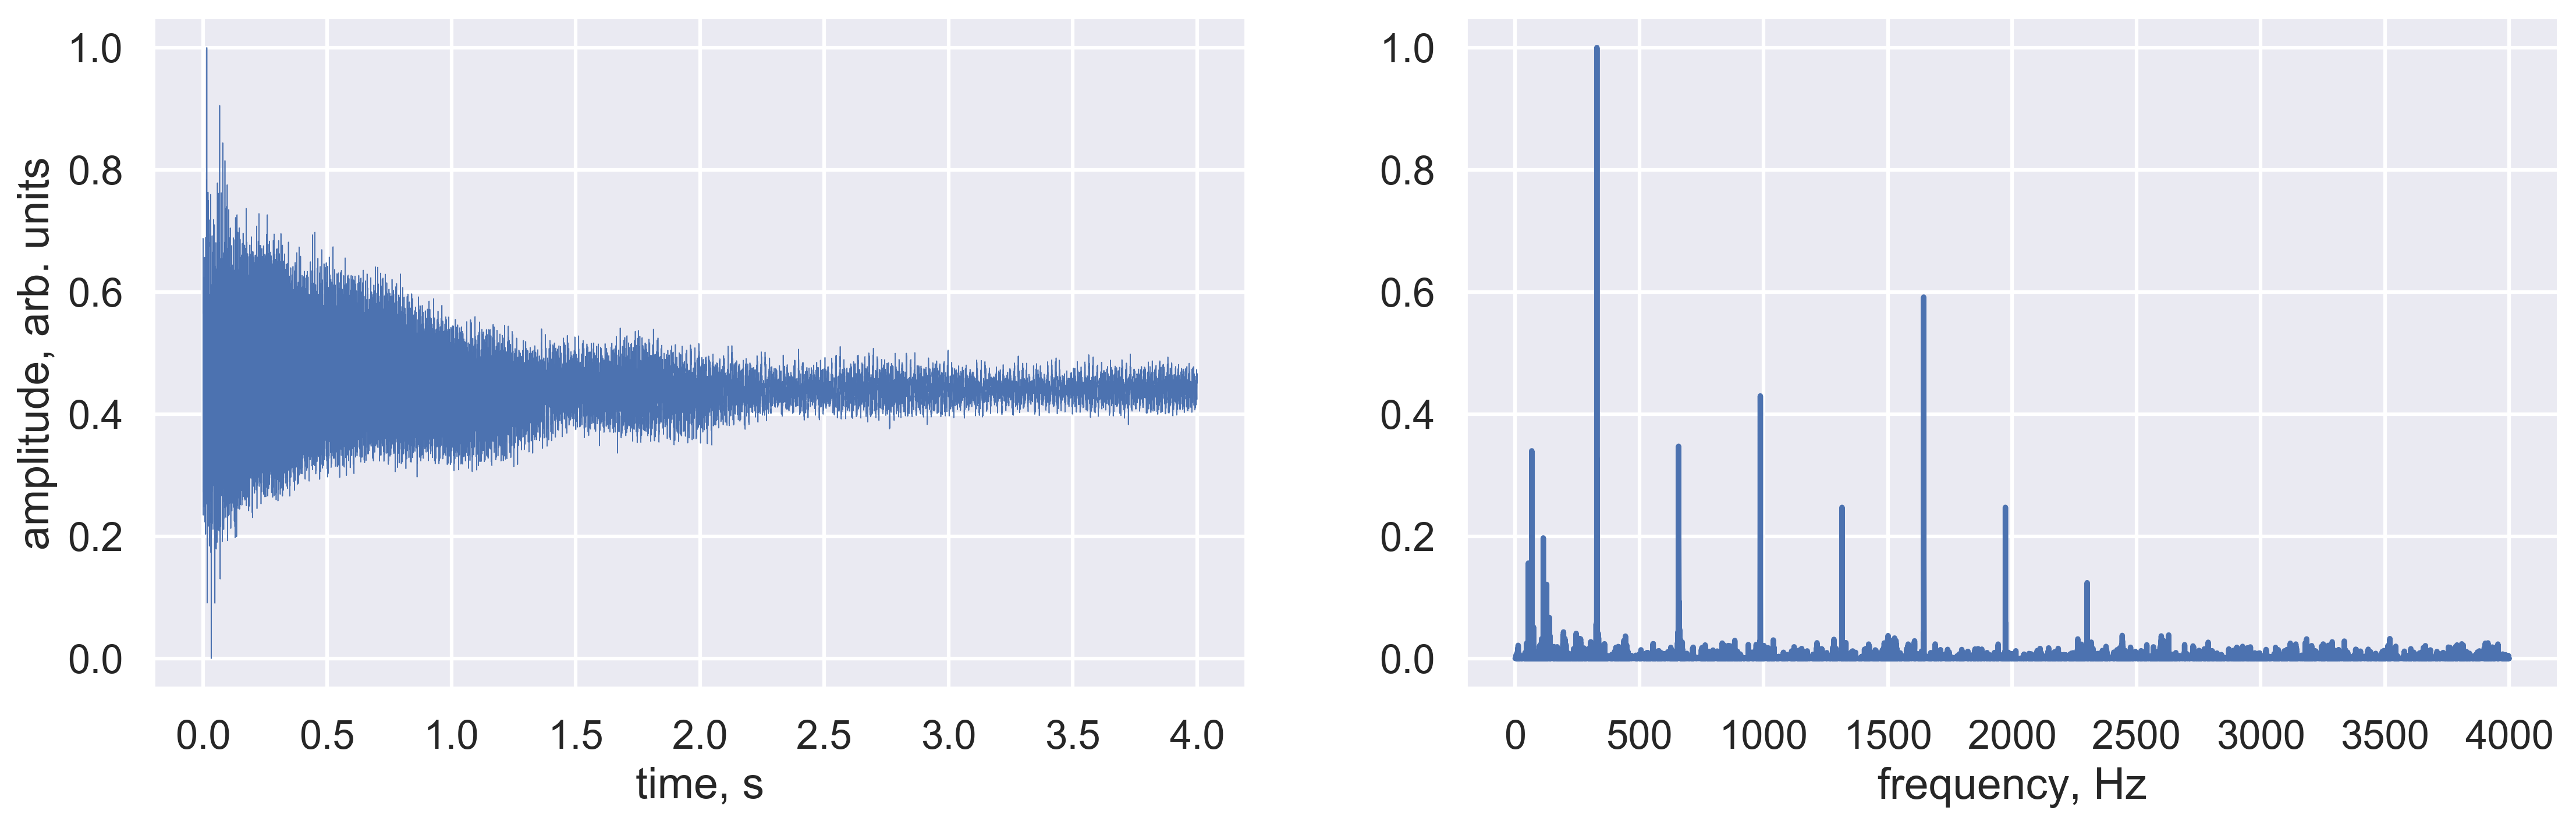
\includegraphics[width=\textwidth]{E1_recov.png}
		\caption{Recovered}
		\label{fig:guitar-recovered}
	\end{subfigure}
	\caption{330 Hz guitar signal representation in the time domain (left column) and frequency domain (right column).}
	\label{fig:guitar}
\end{figure}


\section{Comparison of algorithms}
\label{sec:audio-algorithms}
Following the same procedure as the previous section, my aim now is to compare the performance of three different reconstruction algorithms in terms of average runtime and reconstruction quality. The algorithms used are LASSO and OMP, which were described in Chapter~\ref{chap:theory}. Additionally, the Smoothed L$_0$ Norm (SL0) \cite{Mohimani2009} is used, which approximates the $\ell_0$ norm using a Gaussian of the form

\begin{equation}
\label{eq:sl0}
\lim_{\sigma \rightarrow 0} x \exp\qty(-\frac{x^2}{2\sigma^2}).
\end{equation}

While all algorithms have polynomial time complexity \cite{Efron2004,Sturm2012,Xiang2019}, OMP shows the worst scaling with respect to time; LASSO and SL0 show similar performance over time (Fig.~\ref{fig:guitar-runtime}). In terms of reconstruction quality (cosine similarity), LASSO is able to breach the 0.8 threshold at 30\% compression ratio, while SL0 achieves this at 50\% compression. On the other hand, OMP shows a nonlinear trend with a large error, which is indicative of unstable performance for low compression ratios (Fig.~\ref{fig:guitar-cossim}).

\begin{figure}[htb]
	\centering
	\begin{subfigure}{0.49\textwidth}
		\centering
		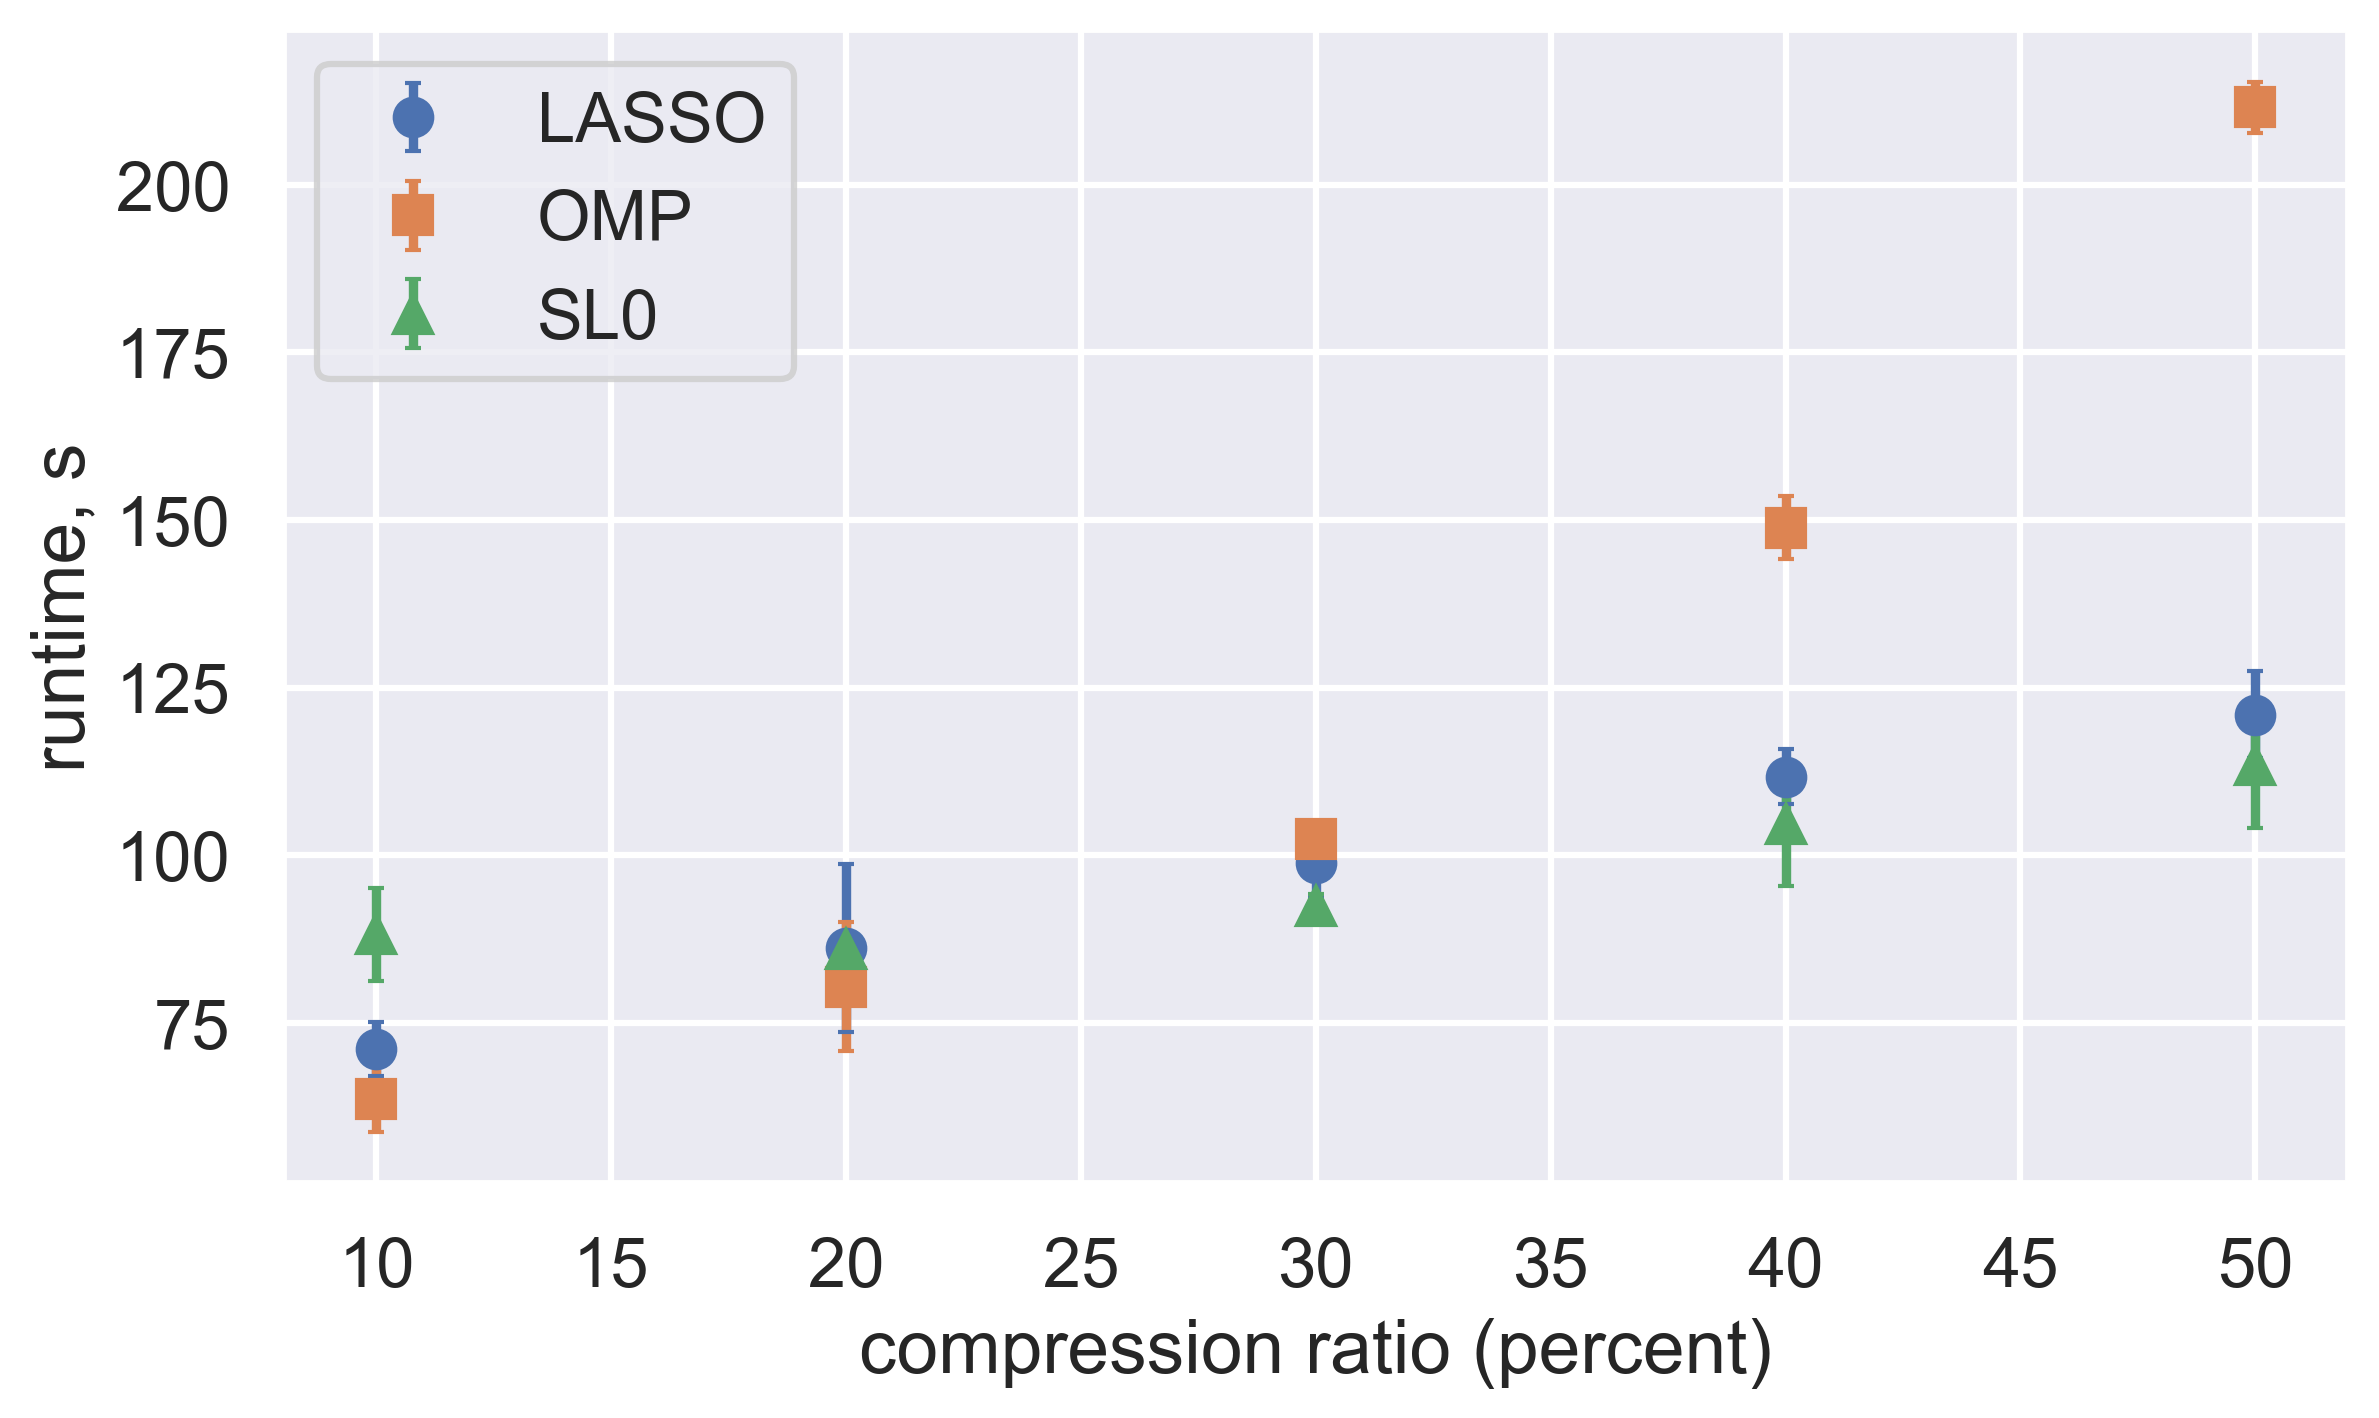
\includegraphics[width=\textwidth]{E1_processtime.png}
		\caption{Runtime}
		\label{fig:guitar-runtime}
	\end{subfigure}
	\begin{subfigure}{0.49\textwidth}
		\centering
		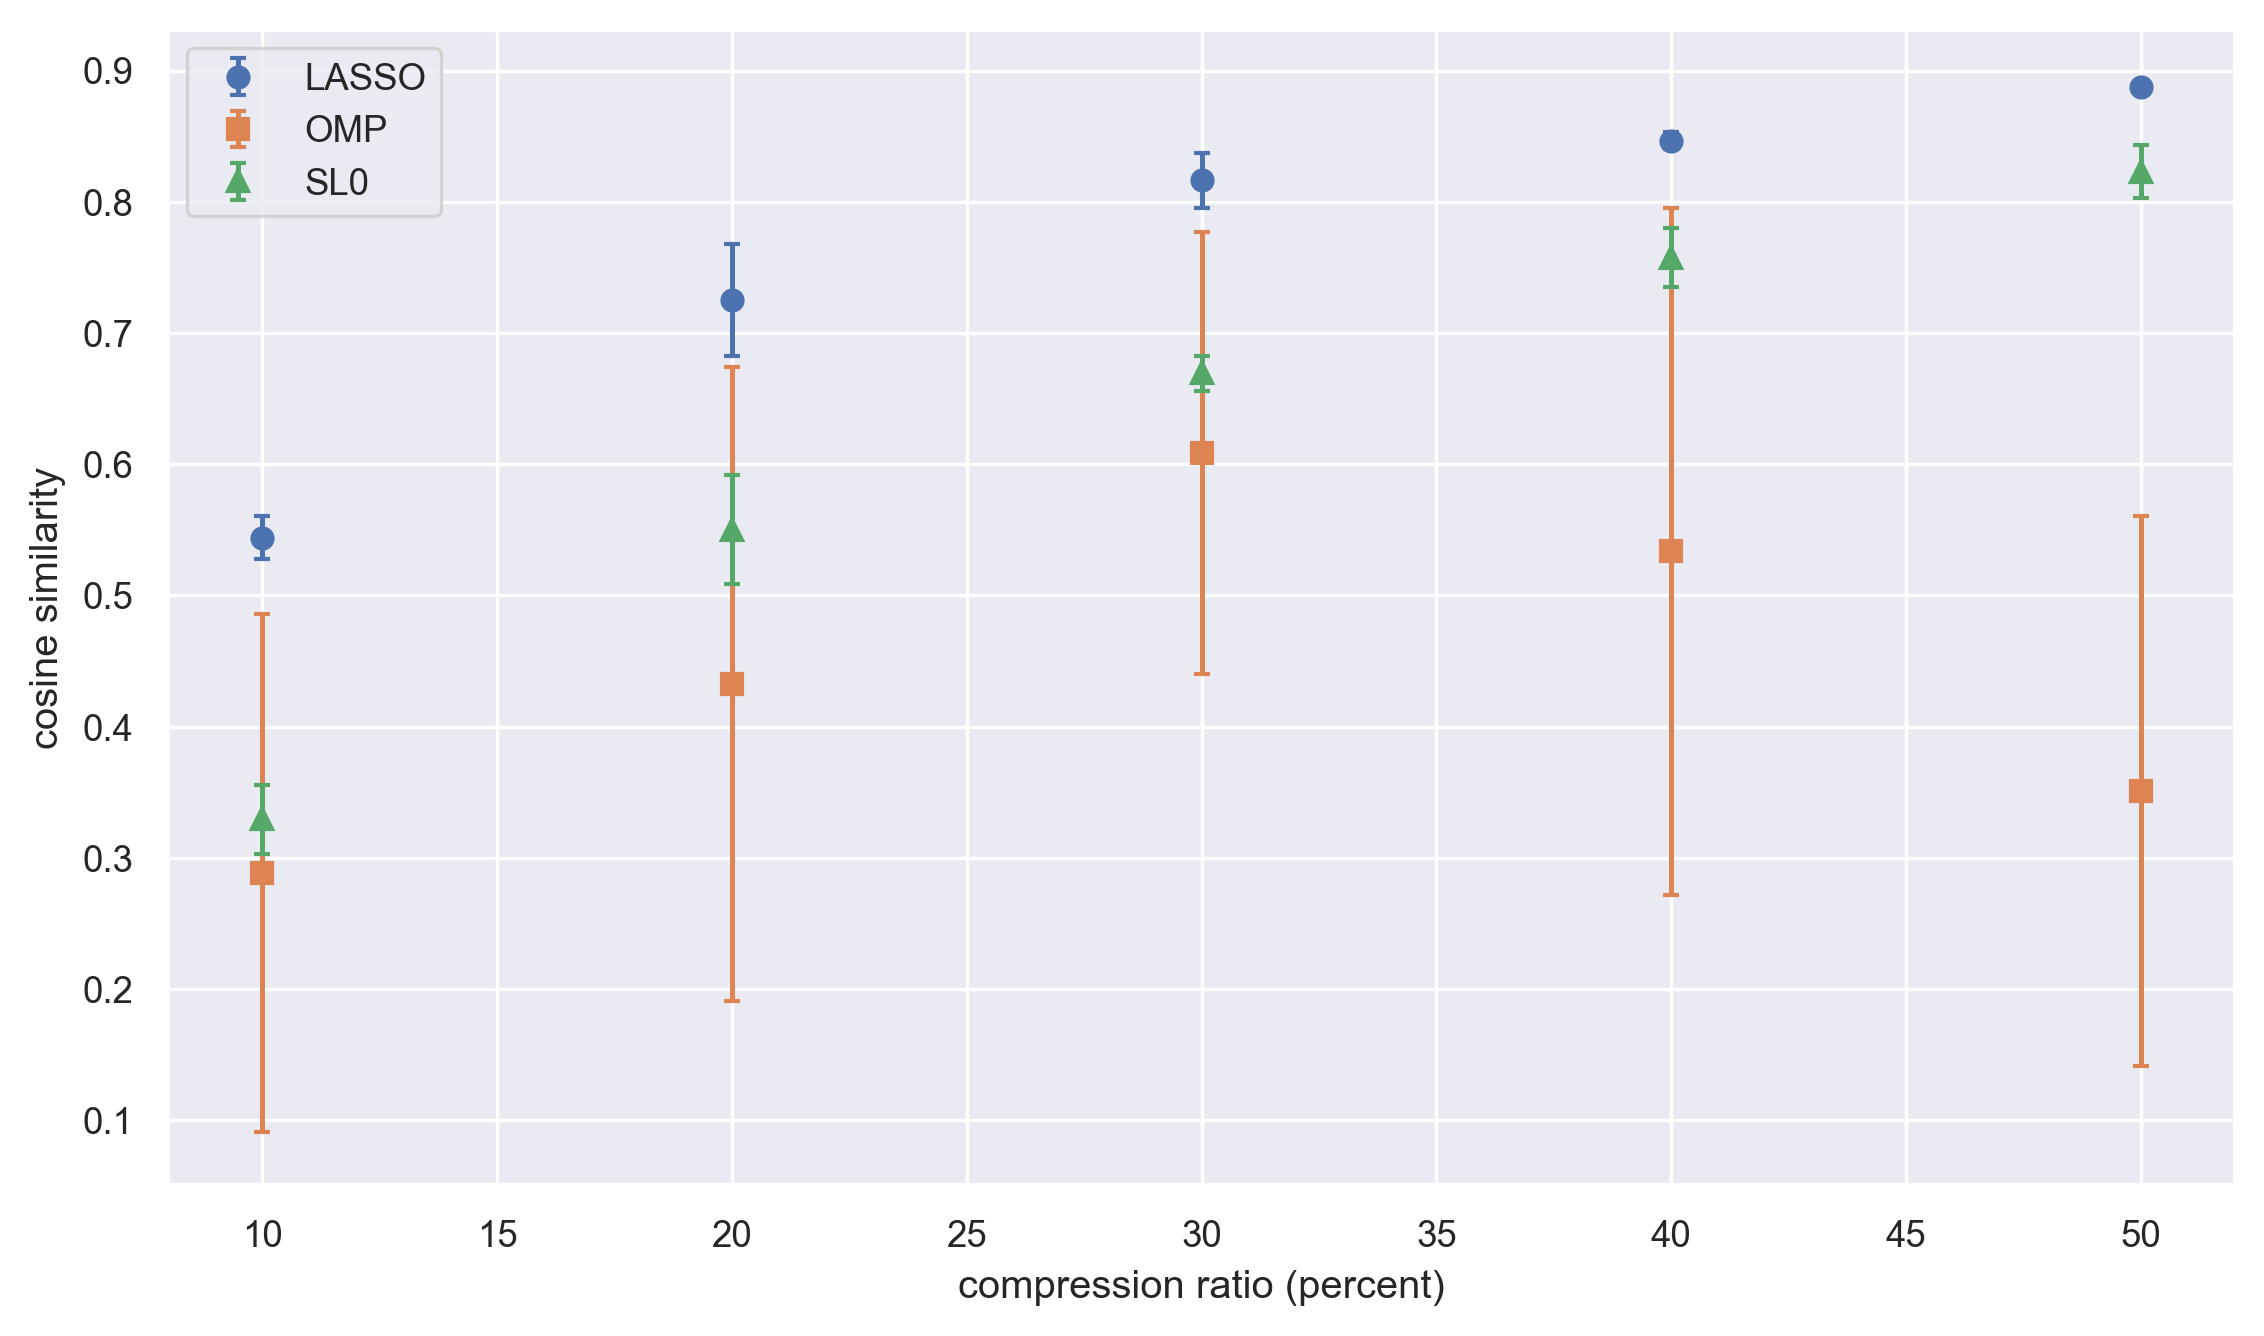
\includegraphics[width=\textwidth]{E1_cossim.png}
		\caption{Reconstruction quality}
		\label{fig:guitar-cossim}
	\end{subfigure}
	\caption{Evaluation of the performance of LASSO, OMP, and SL0 in reconstructing the guitar signal shown in Fig.~\ref{fig:guitar}, in terms of runtime (a) and cosine similarity (b).}
	\label{fig:guitar-algorithms}
\end{figure}


\section{Speech}
\label{sec:audio-speech}
In order to show its practical merits, we will inevitably have to deal with increasingly large and complex signals. Audio recordings containing speech will encompass a wide range of frequencies, so such signals can only be downsampled so much before essential information is lost to aliasing. Unlike images, large audio signals cannot simply be chopped into smaller, manageable pieces. The effects of aliasing are amplified due to the high information density, and CS' violation of periodic constraints introduce artifacts in the vicinity of where the signal was sliced. This is the motivation for transforming the signal first into the modulation domain (spectrogram).

\subsection{Sparse transformation}
\label{ssec:audio-speech-sparse}
In obtaining the spectrogram representation, first define a short length sampling window, typically only a few milliseconds in duration, as well as the overlap between adjacent frames. The latter is crucial in suppressing boundary artifacts as it ensures that some information from the current measurement is carried over to the next measurement. The signal is then divided into frames by sliding this window across the entire signal. Each frame is multiplied with a window function; in this case, I used the Hann window, defined as

\begin{equation}
\label{eq:hann-window}
w[n] = \sin^2\qty(\frac{\pi n}{N})
\end{equation}

\noindent where $N + 1$ is the length of the window, and $n: 0 \leq n \leq N$ is the frame index. Finally, each frame undergoes a Fourier transformation. The entire process is also called a short-time Fourier transform, and is summarized as

\begin{equation}
\label{eq:stft}
X(\omega, p) = \sum_{p=0}^{P-1} x[p] w[p - kR] e^{-i\omega p}
\end{equation}

\noindent where $x[p]$ is the $p$th signal frame, $w[p - kR]$ is the window function with hop size $R$ and time index $k$, and $\omega$ is the angular frequency.

\subsection{Pre-processing}
\label{ssec:audio-speech-preprocess}
Test signals were obtained from the TIMIT Acoustic-Phonetic Continuous Speech Corpus \cite{timit}, which contains speech recordings in \texttt{WAV} format. The recordings are of English speakers grouped by region, sex, and unique spoken sentence. All files have a sampling rate of 16 kHz and are, on average, 3 seconds long. I chose a test signal at random, specifically the \texttt{DR8/MJLN0/SA1.wav} file. This indicates that the speaker was from dialect region 8 (nomadic), was male with speaker code \texttt{JLN0}, and spoke unique sentence \texttt{SA1}, which reads

\begin{quotation}
	She had your dark suit in greasy wash water all year.
\end{quotation}

Before proceeding, I downsampled the file to 8 kHz. The representation of the signal in the time and modulation domains are shown in Fig.~\ref{fig:speech-original}.

\begin{figure}[htb]
	\centering
	\begin{subfigure}{0.49\textwidth}
		\centering
		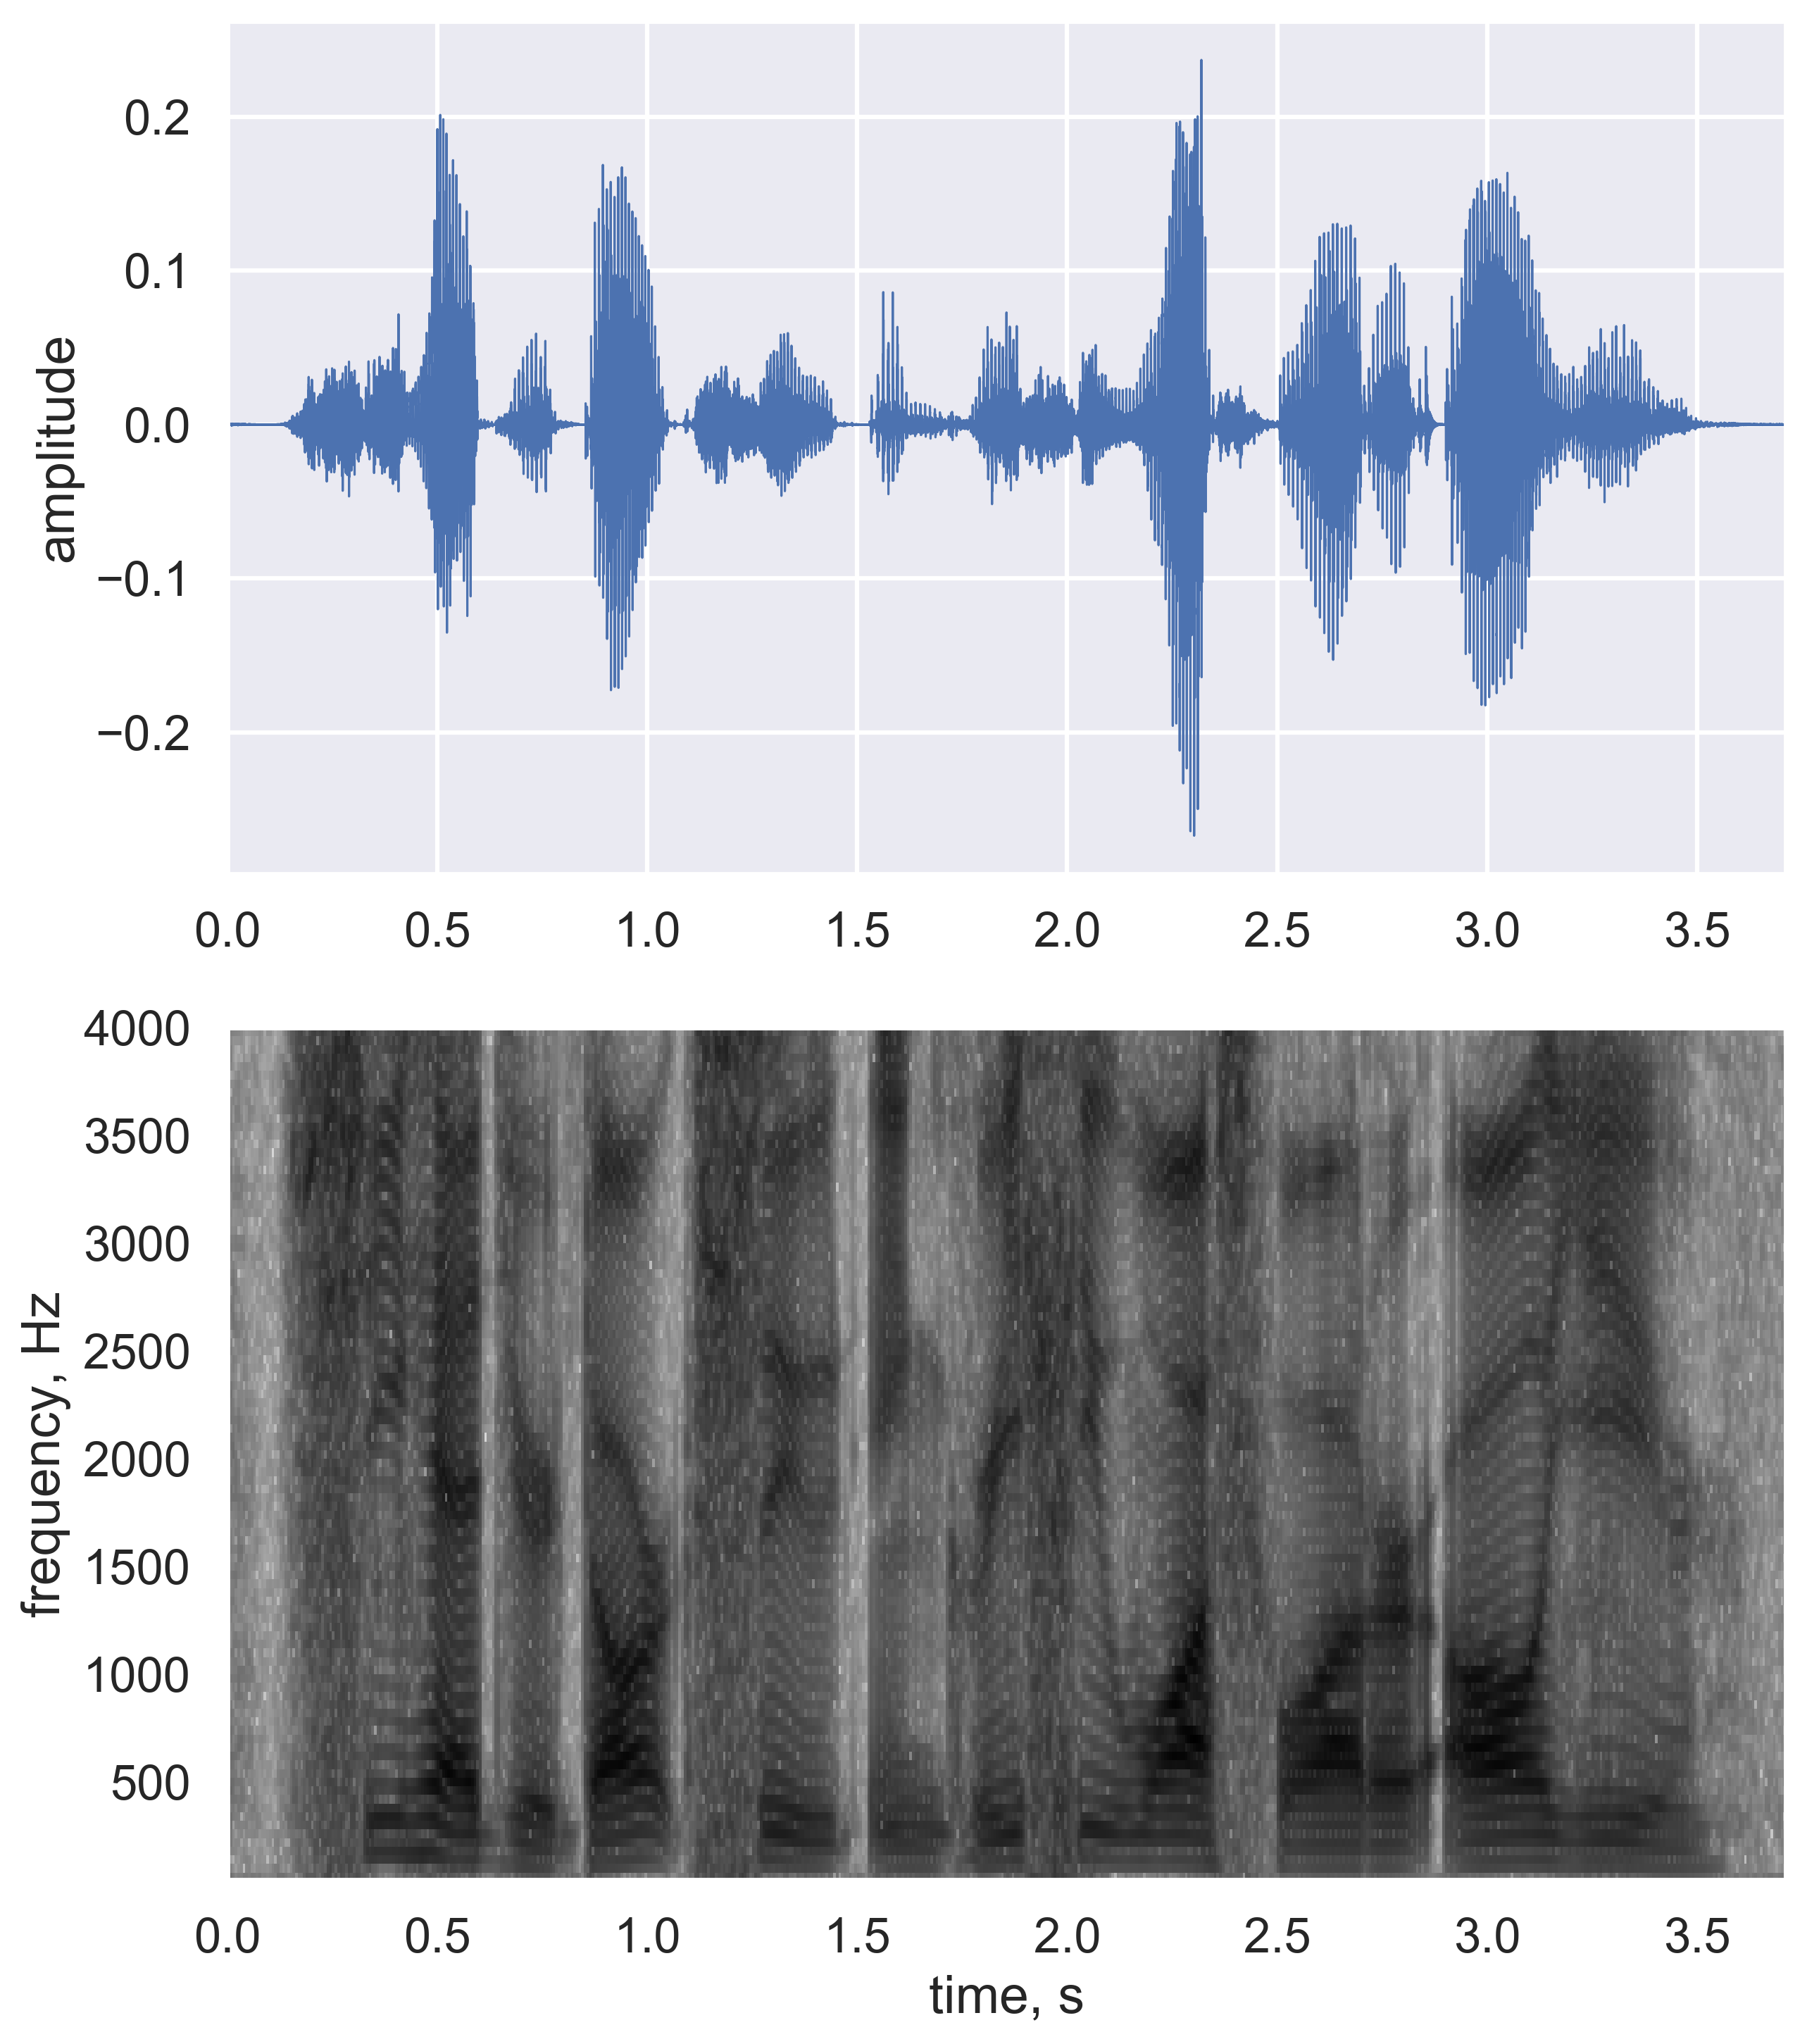
\includegraphics[width=\textwidth]{speech_original.png}
		\caption{Original}
		\label{fig:speech-original}
	\end{subfigure}
	\begin{subfigure}{0.49\textwidth}
		\centering
		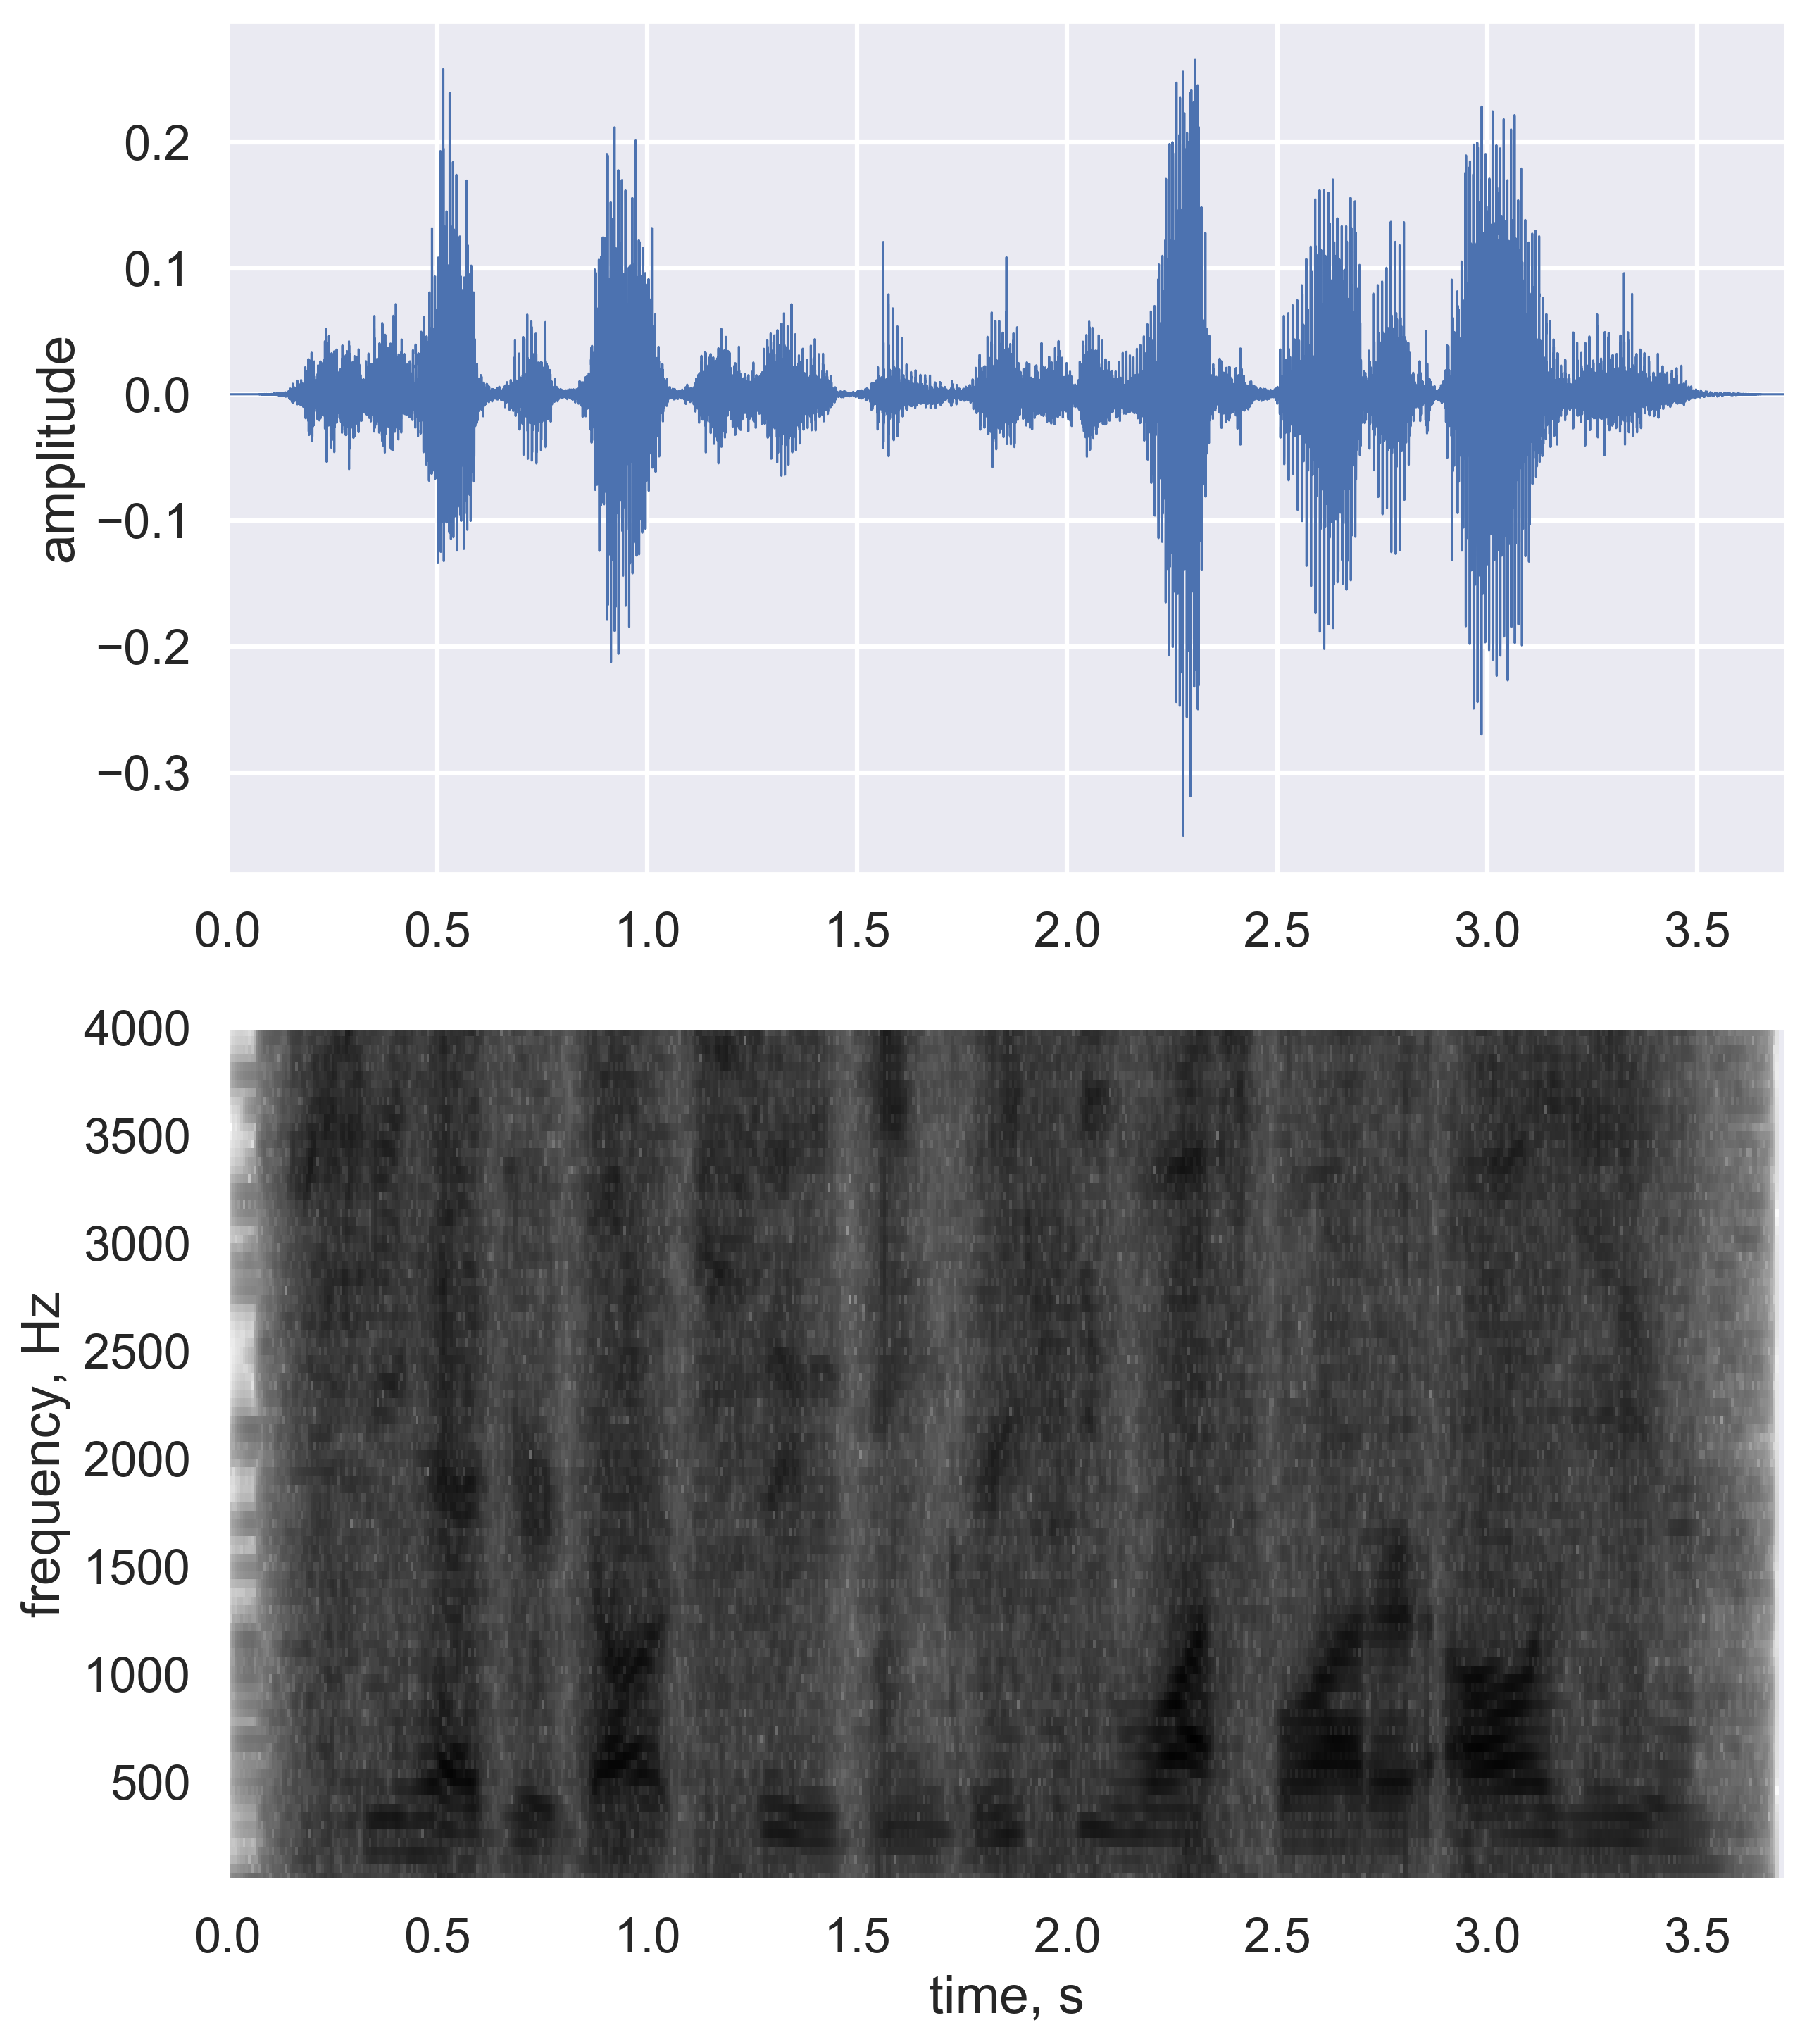
\includegraphics[width=\textwidth]{speech_recover.png}
		\caption{Recovered}
		\label{fig:speech-recovered}
	\end{subfigure}
	\caption{Test speech signal in the time domain (top row) and modulation domain (bottom row).}
	\label{fig:speech}
\end{figure}

\subsection{Processing}
\label{ssec:audio-speech-process}
I compressively sampled the signal with a compression ratio of 40\%, using 1024 frames and 75\% frame overlap. Following the results from Sec.~\ref{sec:audio-algorithms}, I used the LASSO algorithm for reconstruction, once again obtaining the optimal regularization parameter $\alpha$ by 5-fold cross validation.

\subsection{Reconstruction evaluation}
\label{ssec:audio-speech-metric}
The reconstruction quality was quantified using the International Telecommunication Standardization Sector (ITU-T) recommendation P.862 \cite{pesq}, otherwise known as the Perceptual Evaluation of Speech Quality (PESQ). This metric is a full-reference, perceptually intuitive scoring system which models the now-obsolete mean opinion scores (MOS). This algorithm performs a series of standardized tests modeled after qualitative metrics, analyzes and compares the original and reconstructed signals, and returns a value from 1.0 (bad) to 5.0 (perfect). Because real reconstructed signals are rarely exactly the same as the original, the PESQ values are usually thresholded up to 4.5 (excellent). PESQ values of 3.0 and above indicate acceptable quality.

For a more quantitative test, I also used the average segmental signal-to-noise ratio (SNR\textsubscript{seg}) \cite{Loizou2013}, defined as

\begin{equation}
\label{eq:snrseg}
\mathrm{SNR_{seg}} = \frac{10}{B} \sum_{b=0}^{B-1} \log_{10} \frac{\sum_{i = Nb}^{Nb + N - 1} x_i^2}{\sum_{i = Nb}^{Nb + N - 1} (x_i - \hat{x}_i)^2}
\end{equation}

\noindent where $N$ is the frame length, $B$ is the number of frames, $x_i$ are the original signal samples, and $\hat{x}_i$ are the reconstructed signal samples.

Figure~\ref{fig:speech-recovered} shows the reconstructed signal. Qualitative comparison in the time domain shows that the original and reconstructed waveforms are structurally similar. In the modulation domain, the dynamic range of the latter seems to have diminished, but the dominant frequencies can still be observed. Evaluation of the PESQ and SNR$_\mathrm{seg}$ yields values of 2.50 and 0.07, respectively. At face value, I can immediately tell from the PESQ that the reconstructed signal quality is slightly below average; listening to the reconstructed recording reveals a noticeable level of noise in the background. However, the same distinction cannot be made for the SNR$_\mathrm{seg}$ since its bounds are not well-defined.

\subsection{Error space analysis}
\label{ssec:audio-speech-error}
Using the same test signal, I generated the error space maps by compressively sampling the signal and evaluating the metrics for varying compression $\textrm{ratios} \in [0.1, 0.9]$ in increments of 0.1, and varying number of $\textrm{frames} \in \{128, 256, 512, 1024\}$, while keeping the frame overlap constant at 75\%. Figure~\ref{fig:speech-error} shows the PESQ and SNR$_\mathrm{seg}$ maps. The former exhibits a sensitivity to the compression ratio, and achieves the acceptable threshold of 3.0 at around 60\% compression. The latter shows sensitivity towards the number of frames (as it is an \textit{average} metric) with some additional degradation below 40\% compression ratio. It achieves a maximum value of 0.08 at around 1024 frames.

\begin{figure}[htb]
	\centering
	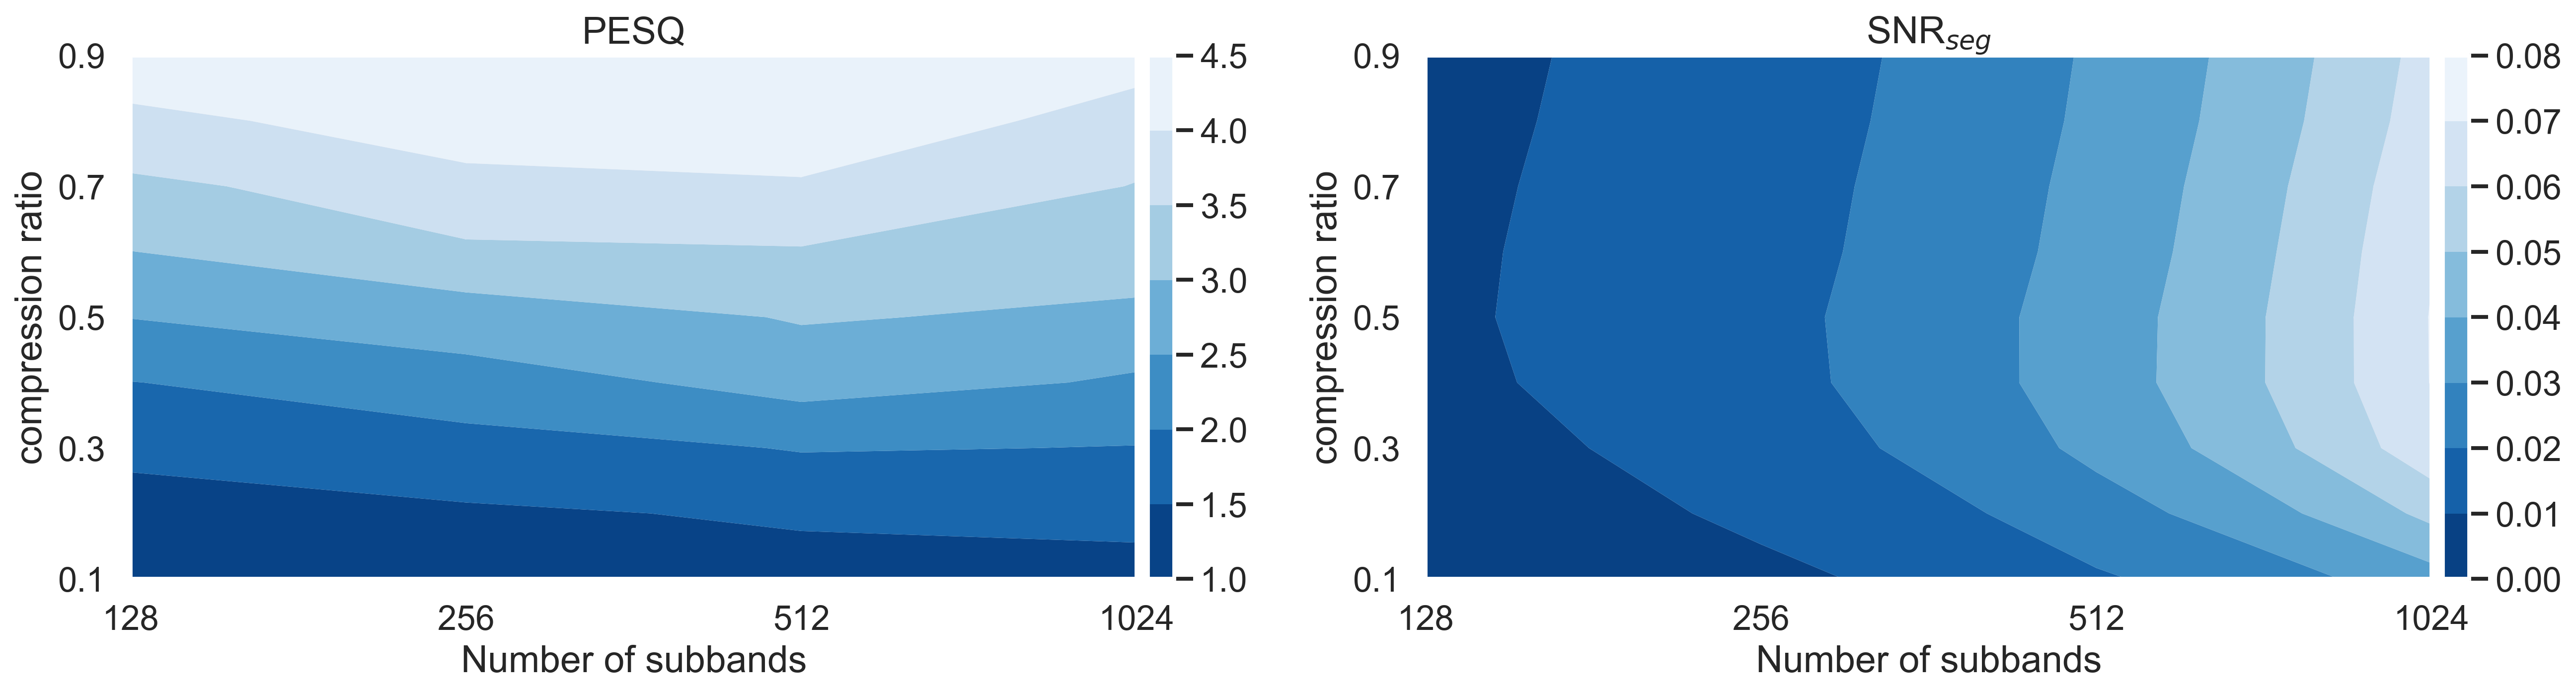
\includegraphics[width=\textwidth]{speech_metrics.png}
	\caption{Evaluation of PESQ and SNR$_\mathrm{seg}$ error space maps as a function of compression ratio and number of subbands, using the same speech recording in Fig.~\ref{fig:speech}}
	\label{fig:speech-error}
\end{figure}
% !TEX root =  main.tex
\chapter{Conclusions and recommendations}
\label{chap:conc}


In this study, I investigated the use of compressive sensing for various applications, and as a viable alternative sampling theorem. In the compressive sampling of signals, there are similar workflows that can be followed separately for image-based and audio-based signals. Both follow a common workflow in the encoding stage, but differ slightly in the decoding stage. Depending on the size of the signal, both types can be processed in one go, but more often than not, the signal has to be processed in several manageable slices. Image-based signals can be sliced into patches with no overlap, while audio-based signals can be divided into subbands with significant overlap in order to suppress reconstruction artifacts.

Due to the sparsity and incoherence requirements of CS, the ideal starting point is by using partial DCT matrices encoded by randomly distributed samples. As for the random distribution, uniform distribution achieves the lowest reconstruction error, while triangular distribution achieves more consistent results throughout a wide range of compression ratios. For this reason, as well as for simplicity in its generation, uniform distribution was used throughout this study. Comparison of three common reconstruction algorithms---namely, LASSO, OMP, and SL0---show that LASSO strikes the balance between run time and reconstruction quality. Thus, this algorithm was used in most cases, except where otherwise stated.

CS is most easily visualized using visual signals. Entire images can be compressively sampled at once if they are small enough. For larger images, they need first be sliced into patches, and each patch can be compressively sampled separately, then stitched back together after reconstruction. Additionally, simultaneous compression and encryption can be achieved using the same algorithms by encoding the sensing matrices with deterministic chaotic functions instead of random distributions. Using a logistic map, the CS compression-encryption system was shown to achieve correlation coefficients of as low as 0.02, and no higher than 0.42. Key sensitivity analysis showed that the system was sensitive to initial value perturbations on the order of $10^{-15}$, making it robust against brute force attacks. The structural similarity index (SSIM) was determined to be a perceptually accurate metric for this type of signal, and a value of 0.8 and above is deemed acceptable. The experiments performed in the study achieved reconstruction errors of no lower than 0.82 SSIM.

Denser signals, such as audio, benefit largely from CS. Undersampling artifacts are more easily apparent in these signals. If the signal is simple enough, i.e., those with relatively unchanging frequencies, then it can be processed all at once. The same procedure with image-based CS can be followed, but in addition, the slicing the signal into subbands (analogous to image patches) require some overlap between adjacent subbands in order to suppress undersampling artifacts. Experiments with recordings of single guitar notes showed that even while undersampling just enough to capture the base frequency of a note, up to sixth-order harmonics can still be recovered using CS. For larger and complex signals such as speech, it may be necessary to transform the signal to a higher dimension where it can be represented more sparsely, i.e. from the temporal domain to the modulation domain. A speech recording of a complete sentence was compressively sampled successfully with a 40\% compression ratio, and 75\% overlap between adjacent subbands. Error space mapping in terms of PESQ and the more widely used average segmental SNR (SNR$_\mathrm{seg}$) shows that the reconstruction quality of a signal in terms of PESQ can solely be described by the compression ratio, while in terms of SNR$_\mathrm{seg}$, by the number of subbands used to divide the signal. The perceptual evaluation of speech quality (PESQ) was determined to be a perceptually accurate metric for this type of signal, and a value of 3.0 and above is deemed acceptable. The experiments performed in the study achieved reconstruction errors of no lower than 2.5, which is quite lower than the acceptable threshold.

Future studies may look into further standardizing the CS workflow by introducing overlap between adjacent image patches---similar to audio---to improve reconstruction quality. For audio-based signals, one may explore varying parameters such as compression ratio, percent overlap, and number of subbands to also improve reconstruction quality. Finally, all these can be combined to compressively sample signals which may contain any combination of audio and images, such as full HD color videos and hyperspectral images.
%% you may add more chapters by including more files just as above.
%% see the files for patterns of the format used.

\appendix
\chapter{Codes and Implementations}
\label{appendix:codes}

\singlespacing
\lstset{
	basicstyle=\footnotesize\ttfamily,
	commentstyle=\itshape\color{green!50!black},
	keywordstyle=\bfseries\color{Purple},
	stringstyle=\color{red!70!black},
	numberstyle=\footnotesize\ttfamily,
	numbersep=15pt,
	tabsize=4,
	frame=lines,
	language=Python,
	numbers=left,
	label={code:1d-test},
	caption={Code for compressive sensing of 1D test sinusoids.}
}
\lstset{morekeywords={as, True, False}}
\begin{lstlisting}
import numpy as np
import numpy.random as rand
import scipy.fftpack as fft

# load recording
signal = np.loadtxt("piano.txt").astype("float32")

# define parameters
samprate = 44.1e3
duration = 1/8
N = int(duration*samprate)
M = 300
t = np.linspace(0, duration, N)

# extract short portion of recording
sig_start = 40000
x = signal[sig_start:sig_start + N]

# simulate compressive measurements
yi = rand.randint(0, N, M)
yi = np.sort(yi)
y = x[yi]

# L1 optimization using CVX ECOS
import cvxpy as cvx
xhat_cvx = cvx.Variable(N)
objective = cvx.Minimize(cvx.Norm(xhat_cvx, 1))
constraints = [A*xhat_cvx == y]
prob = cvx.Problem(objective, constraints)
result = prob.solve(verbose=True, solver="ECOS")
x_cvx = np.array(xhat_cvx.value)
x_cvx = np.squeeze(x_cvx)
x_cvx = fft.dct(x_cvx, norm="ortho", axis=0)

# L1-regularized L2 optimization using LASSO
from sklearn.linear_model import Lasso, LassoCV
lasso = LassoCV(cv=10, random_state=0, verbose=True, n_jobs=-1)
lasso.fit(A, y)
x_lasso = fft.idct(lasso.coef_)
\end{lstlisting}

\lstset{
	label={code:random},
	caption={Code for generating different random distributions.}
}
\begin{lstlisting}
from sklearn.metrics import mean_squared_error
# define parameters
samprate = 44.1e3
duration = 1/32
N = int(duration*samprate)
M = np.arange(50, N+1, 50)
t = np.linspace(0, duration, N)

# define normalization function
def normalize(x):
	x = x.astype(float)
	x /= x.max()
	return x

# evaluate errors
y_uniform_errs = []
for m in M:
	trial_err = []
	for i in range(10):
		yi = rand.uniform(0, N, m)
		yi = np.sort(yi)
		y_uniform = signal[yi]
		d = np.identity(N)
		d = fft.dct(d)
		A = d[yi]
		lasso = Lasso(alpha=0.1)
		lasso.fit(A, y_uniform)
		xhat_uniform = fft.idct(lasso.coef_)
		mse = mean_squared_error(normalize(signal), normalize(xhat_uniform))
		trial_err.append(mse)
	y_uniform_errs.append(trial_err)
\end{lstlisting}

\bibliographystyle{plain}
\bibliography{library,thesis} %% see file: "biblio.bib"

\end{document}
%%end of main.tex
